\documentclass[11pt]{report}
\usepackage{tikz}
\usepackage{graphicx} \DeclareGraphicsExtensions{.eps} \graphicspath{{bilder/eps/}}
\usepackage{url}
\usepackage[backend=biber,
            style=ieee,
            maxbibnames=20]{biblatex} % to generate the bibliography
\addbibresource{bachelorthesis.bib}           % name of the bib-file

%definition of page size etc
\setlength{\textwidth}{15 true cm}
\setlength{\textheight}{22 true cm}
\oddsidemargin  0.5 cm
\evensidemargin 0.5 cm
\topmargin      0 cm


\begin{document}

% -----~* TITLE PAGE *~-----
\begin{tikzpicture}[remember picture,overlay]
  \node[xshift=30mm,yshift=00mm,anchor=north west] at (current page.north west){%
  
\includegraphics[width=10mm]{img/general/iti_logo.png}};
\end{tikzpicture}
\hfill
\begin{tikzpicture}[remember picture,overlay]
  \node[xshift=-30mm,yshift=-20mm,anchor=north east] at (current page.north east){%
  
\includegraphics[width=50mm]{img/general/tuglogo.eps}};
\end{tikzpicture}

\begin{center}
\vskip6cm
\fontsize{24pt}{32pt}\selectfont Bachelor Thesis \par
\vskip1.8cm
\fontsize{48pt}{36pt}\selectfont \textbf{Automotive Cyber Security:} \par
\vskip0.3cm
\fontsize{32pt}{32pt}\selectfont Try out hacking and \\ 
service tools available for \\
automotive communication \par
\vskip6.4cm
\fontsize{18pt}{20pt}\selectfont Peter Fürlinger \par
\end{center}

\newpage
%  -----~* TABLE OF CONTENTS *~-----
\setcounter{tocdepth}{2}
\tableofcontents  

% -----~* ABBILDUNGSVERZEICHNIS *~-----
\listoffigures
\pagestyle{headings}

% -----~* INTRODUCTION *~-----
\chapter{Introduction}

\section{Communication Attacks}
As cars are outfitted with more and more sensors, actuators and control modules, the complexity of communication inside a vehicle rises dramatically as well. A car made today can include as many as 60 control units and the electronics inside the vehicle can account for over 20\% of the manufacturing costs. 

As the flow of information inside a vehicle increases, protecting this information from attackers is becoming increasingly important. Otherwise, so-called communication attacks may be carried out by unauthorized parties in order to gather information about or even control over critical systems inside a car. These attacks are a major problem in the automotive sector, which is why regulators and manufacturers have the common goal of preventing them. In order to recreate or prevent such attacks, a substantial amount of documentation about them is needed. Known exploits are thoroughly documented and shared to the public by the aforementioned entities.

This thesis will cover how to gather information about such exploits, how to recreate them as well as which tools are the best fit for such a task. Additionally, a small demonstration will be included.

\section{Difference between safety and security}
When discussing vulnerabilities, there is an important distinction to make regarding the ways corrupt of a system. It can be either compromised in its security or its safety. 
Exploiting a system's security can mean exploiting its confidentiality or integrity. An attacker might gain access and/or control over a system, extract protected data or maliciously disable a systems reliability and availability even though they are not allowed to by exploiting system security.
Exploiting the systems safety means causing harm to people and the environment via a malfunctioning system. 
Additional care by a systems designers and engineers needs to be taken to ensure the protection of users in case a system malfunctions, especially if it was made to malfunction by a malicious party on purpose. 
An example of this would all considerations regarding what might happen when a vehicle in motion is remotely turned off or loses one or more of its sensors. In order to ensure adequate safety, the security provided needs to be adequate as well.

\section{Prevention by the governments, UN and NCAP}
There are numerous agencies whos mission it is to improve vehicle safety. Since communication attacks not only present a security, but often also a safety risk, these entities are continuously working in collaboration with the automotive industry to prevent these types of attacks. Due to the fact that vehicle safety is often closely related to road safety, these types of agencies tend to be created by individual countries or a group of cooperating countries. While road laws are still usually passed and enforced by individual countries, or in the case of the United States on a state-level, these agencies can often influence the qualifications needed by new road cars in order to be registered for public use and therefore influence the entire industries safety standard.

\subsection{National Highway Traffic Safety Administration}
One of the most important examples of this is the National Highway Traffic Safety Administration. It is a part of the Department of Transportation (DoT) of the United States Federal Government. Since the US is the second-largest automobile manufacturer in the world according to the European Automobile Manufacturers' Association,\cite{acea} and all vehicles on american roads have to adhere to the laws made by its government, the DoT and by extension the NHTSA are an important influence on the design of new cars. The NHTSA regularly gives out Federal Motor Vehicle Safety Standards.\cite{nhtsacybersec} %TODO bessere citation?
In 2022, the NHTSA released an updated version of the  the ``Cybersecurity Best Practices for
Modern Vehicles'' (originally released in 2016). While this is not technically a regulation, it presents the industry with a guide for improving vehicle cybersecurity as a whole.\cite{nhtsabestpractice}

\subsection{World Forum for Harmonization of Vehicle Regulations}
The european equivalent of the NHTSA would be the World Forum for Harmonization of Vehicle Regulations (UNECE WP.29), which is an arm of the United Nations Economic Commission for Europe. It is reponsible for managing an agreement between 64 countries on the general standard for vehicle safety regarding construction, approval and periodic safety inspection for continuous road use. If new technology is developed or a new safety risk is discovered, new regulations are passed in the form of an appendage to the original agreement from 1954.
Participating countries include the entire European Union as well as non-ECE states such as Thailand and Pakistan. Notable absentees from the list of participating countries are the US and Canada. The former has developed their own standard as mentioned, while the latter has their own system of rules called Canada Motor Vehicle Safety Standards. \cite{unece} %TODO bessere citation?
In August of 2020, the UN ECE adopted two new regulations regarding cyber security and software updates in road cars (R155 and R156 respectively). These regulations will only take effect once each participating country has implemented them into their road laws. Since the European Union has already issued mandatory compliance dates for all new vehicles, the adoption of these regulations likely will be completed by January 7th 2024 at the latest.

\subsection{Euro NCAP}
Another notable example of such an entitiy is the European New Car Assesment Programme, which was created in 1996 in order to produce studies and safety ratings for road cars in the European Union. As opposed to the NHTSA, which is able to directly enforce laws, the NCAP merely produces a rating system on the safety of cars. While the NCAP's main focus lies on crash testing, they are also working on an Automotive Cyber-Security Standard, which will help manufacturers secure their vehicles against these kinds of communication attacks. The Euro NCAP will monitor the development of these standards and regulations and may even require a minimum level of security from a manufacturer.\cite{ncaproadmap}

\section{Vulnerability Databases}
In order to share information about vulnerabilities and make them easier to classify and compare, known vulnerabilities are often collected in databases, where they can easily be catalogued and looked up. These databases are usually collected and maintained either by companies or by non-profit organizations and can be accessed either for free or require payment.
\subsection{Open Source Vulnerability Database}
One example of such a database is the ``Open Source Vulnerability Database'', which was founded in August of 2022 as part of the Black Hat and DEFCON Conferences by attendees well-known in the security industry.
To this day, this project is still entirely maintained by volunteers, including some from a company called ``Risk Based Security''.
%TODO better citation
\subsection{MITRE CVE List}
CVE is the abbreviation for common vulnerabilities and exposures. A CVE describes 
%TODO better citation
These CVEs are usually compiled in a searchable list by so called CVE Numbering Authorities (also known as CVEs).
\subsection{National Vulnerability Database}
The National Vulnerability Database is maintained by the US government and is among other things fed by the MITRE CVE list. In addition it also features a Common Vulnerability Scoring System (CVSS) for each of its entries. A study in 2017 found the delay between a CVE being discovered and it's admission into the NVD to be about seven days, thus giving hackers a window of oppurtunity to exploit it, since they are often published unofficially before.

%R155 regulations dokumentieren

% -----~* RESSOURCES *~-----
\chapter{Ressources}
\section{Software Tools}
\subsection{Tools for Traffic Monitoring Fingerprinting}
\subsubsection{Vehicle Spy}
Vehicle Spy is a proprietary software developed and sold by Intrepid Control Systems. It is capable of reversing many vehicle communication protocols, including CAN. It is capable of bus monitoring, simulation, diagnostics, memory manipulation and more.
%TODO cite https://intrepidcs.com/products/software/vehicle-spy/

\subsubsection{Linux Tools (can-utils)}
Linux supports CAN out of the box and comes packaged with many useful command line utilities to simplify working iwht the CAN bus. The package containing these userspace utilities is called ``can-tools''.

%TODO cite Car Hackers Handbook page 360
%TODO cite https://github.com/linux-can/can-utils
Its features include but are not limited to the following:
\begin{itemize}
    \item displaying, generating, recording and playing back CAN messages
    \item access CAN Bus via IP sockets
    \item bus measurement and testing
    \item log file conversion
    \item CMake project generation
\end{itemize}
%TODO make sure bus is spelled lowercall all the time

\subsubsection{CANTools/python-can}
``cantools'', also known as CAN BUS Tools, is a library for python3, which allows encoding and decoding CAN Bus Messages as well as diagnostic DIDs. On top of that it also simplifies parsing files that store recorded CAN messages like DBC, KCD and many more file types.
It can be installed by simply running the following command (assuming pip is set-up on the system):
\begin{verbatim}
    python3 -m pip install cantools
\end{verbatim}
In order to actually send and receive messages over a CAN bus another python library called ``python-can'' can be used. This library can also be installed with pip:
\begin{verbatim}
    pip install python-can
\end{verbatim}
%TODO cite https://github.com/cantools/cantools
%TODO cite https://python-can.readthedocs.io/en/master/

\subsubsection{Wireshark} \label{wiresharkintro}
Wireshark is a free and open source packet analyzer available for Unix and Windows Systems. Packet analyzers can be used to examine network traffic in great detail on a packet level or even as raw data. Wireshark is one of the most commonly used applications for this purpose and often referred to as the de facto industry standard.
%TODO cite https://www.wireshark.org/docs/wsug_html_chunked/ChapterIntroduction.html#ChIntroWhatIs

The software has been continually expanded and developed for use with new protocols since 1997. It currently supports hundreds of protocols including CAN, bluetooth and many more that are commonly used in automotive applications.
%TODO cite https://www.wireshark.org/docs/wsug_html_chunked/ChIntroHistory.html
%TODO cite https://www.wireshark.org/docs/dfref/

It supports live data capture from a network interface as well as analyzation of previously recored files. A big benefit of Wiresharks user interface is that packets can be searched, filtered and colorized based on a number of properties, making the visualization of the captured data incredibly easy. In addition to that, packet data can also be saved and exported in a number of formats.
%TODO cite https://www.wireshark.org/docs/wsug_html_chunked/ChapterIntroduction.html#ChIntroFeatures

%\subsubsection{O2OO Data Logger}
%no longer exists

%\subsubsection{Kayak}
%no longer exists

\subsubsection{Caring Caribou}
Caring Caribou is a sort of penetration testing tool for the automotive space. It is comprised of different modules designed to test different components of a vehicles CAN implementation.

Among many others, Caring Caribou provides a lot of useful features meant to discover security vulnerabilities in a CAN system such as the following:
\begin{itemize}
    \item scan for ECUs supporting diagnostic services
    \item scan for diagnostic services supported by an ECU
    \item reset an ECU
    \item dump ECU memory (such as SRAM, flash and bootloader) to file
    \item scan for ECUs supporting Universal Measurement and Calibration Protocol (XCP)
    \item fuzzing CAN (sending random CAN messages and brute forcing)
    \item dumping CAN messages
    \item send CAN Messages
    \item listen for CAN messages
    \item run automated test suites
\end{itemize}

\subsubsection{SavvyCAN}
SavyCAN is a free and open source GUI utility designed to simplify reverse engineering and capturing CAN data. The biggest advantage of this tool compared to other packet analyzers is the ability to connect multiple dongles simultaniously and the ability to capture data from very busy bus systems. It additionally also supports many useful file operations from log files such as DBC as well as reverse-engineering capabilities like scanning and decoding diagnostic messages, monitoring traffic from the radio, sniffing the vehicles identification number (VIN) and much more.
%TODO cite https://www.savvycan.com/

\subsubsection{c0f Fingerprinting Tool}
This utility can be used to create a fingerprint data traffic of any vehicle just by passively monitoring its CAN messages. This is done by first monitoring about 2000 or more CAN messages using candump (which is part of can-utils mentioned above) or similar. Once this is completed c0f returns JSON data with a lot of useful information like which signals tend to repeat often, the signal with the highest interval rate and said interval rate.

This information can then be added to a database. In the future the developer Craig Smith also plans on shipping the software with a fingerprint database included.
%TODO cite https://github.com/zombieCraig/c0f

\subsection{Communicating with the CAN Bus}
\subsubsection{PyOBD Module}
PyOBD is a car diagnostics tool written entirely in python and a fork of pyOBD developed by SECONS Ltd. It is designed to be used specifically with ELM32x interfaces, which were described above. It is capable of displaying and clearing fault codes, reading live sensor data and reading status tests.
%todo cite https://github.com/chethenry/pyOBD


%\subsubsection{CANiBUS Server}
%very niche and also archived + read only so probably discontinued

%\subsubsection{AVRDUDESS GUI}
%not automotive specific + weird


\subsection{ECU Simulation and Tuning}
\subsubsection{UDSim ECU Simulator}
%https://github.com/zombieCraig/UDSim

\subsection{Instrument Cluster Simulator for SocketCAN}
%https://github.com/zombieCraig/ICSim

%\subsubsection{RomRaider ECU Tuner}
%subaru engine only

\section{Hardware Tools}
\subsection{Software Defined Radio for Radio and RFID attacks}
A software defined radio is a device capable of sending and receiving radio signals on various frequencies. As opposed to a traditional radio tranceiver, which is made up of analog components, a software defined radio is comprised of only an RF front-end and a digital-to-analog converter (DAC). All of the signal processing, which usually happens in dedicated analog hardware is instead passed off to a general-purpose CPU. This enables the device to communicate over a multitude of different radio protocols.

There are a number of different SDRs on the market. They can be characterized by a number of different factors. The most important property of such a device is the frequency band it operates on. While cheap units can often cover ranges up to 1GHz, devices capable of higher frequency ranges are often more expensive. Another important distinction is whether or not the device is capable of sending signals or just receiving them. The third important classification of SDR is the range it is capable of transmitting over.

SDRs can be used to tune into a specific frequency and capture traffic. An attacker might use this to capture, record, alter or play back any RFID signal used by a vehicle. This is also called a ``Replay Attack'', which will be demonstrated later.

\subsubsection{ADALM-PLUTO}
ADALM is short for ``Analog Devices Active Learning Module'', which is Analog Devices' line-up of products designed specifically for students and hobbyists. While they are meant to be used with AD's free educational exercises, they are no less feature packed than an off-the-shelf device. Due to the nature of them being learning tools, devices in this lineup are typically very affordable.
%TODO cite https://www.analog.com/media/en/news-marketing-collateral/solutions-bulletins-brochures/active-learning-program-for-students.pdf

The ADALM-PLUTO is a software defined radio capable of covering a frequency spectrum from 325MHz to 3.8GHz, with up to 20MHz of instantaneous bandwidth. It is able to transmit as well as receive in half or full duplex mode and is very well expandable due to its Matlab Simulink support as well as C, C++, C\# and Python API. It also comes with two antennas, which greatly increases its range.
%TODO cite https://www.analog.com/en/design-center/evaluation-hardware-and-software/evaluation-boards-kits/adalm-pluto.html

\subsubsection{HackRF SDR}
The HackRF SDR is another creation from Great Scott Gadgets, which is also the manufacturer of the Ubertooth One. It is a software defined radio designed to be a successor to the Ubertooth, which was discontinued on 22.12.2022 and greatly expands on its capabilities.

It is able to transmit in half-duplex mode only to ensure coverage of most SDR use cases, while still being cost effective. It transmits in a range of 1MHz to 6Ghz. It comes with a powerful software utility, but is also compatible with GNU Radio, SDR\# and more. It can also be configured to operate without a host computer in stand-alone mode.
%https://greatscottgadgets.com/hackrf/one/

The HackRF does not ship with an antenna, but features SMA connector so they can be bought seperately and connected.

\subsubsection{USRP SDR}
Universal Software Radio Peripheral (USRP) is a lineup of SDR devices manufactured by Ettus Research, a brand of National Instruments.
%TODO cite https://www.ettus.com/

Much like the ADALM family of products, it is primarily designed with hobbyists and university students in mind. The devices in this line-up starts from business card sized SDRs costing a few hundred USD up to powerful rackmounted systems with a price point of around 20.000 USD or more.

Along with batteries and cables, antennas can be purchased seperately, as most of these devices feature SMA ports. Daughterboards are also offered to expand the more higher-end SDRs even more.
%TODO cite https://www.ettus.com/products/

\subsection{Bluetooth Devices}
\subsubsection{UbertoothOne} \label{ubertoothintroduction}
Specific Hardware is needed in order to capture and demodulate Bluetooth Signals. One such device is the ``Ubertooth One'', made by Great Scott Gadgets. It was originally conceived by the company's founder Michael Ossmann.\cite{ubertoothabout}
It is available from multiple vendors, because it is a fully open source device, both in hardware and software terms. This also makes it very affordable.
It is capable of capturing signals in the 2.4GHz ISM Band, which ranges from 2.4GHz to 2.5GHz and is commonly used for wireless networking. The device is able to transmit and receive in this range with a fairly narrow bandwidth of 1MHz.\cite{ubertoothfaq} ISM is the abbreviation for ``industrial, scientific and medical'', which is an unlicensed short range radio frequency band. Since Bluetooth transmits between 2.4GHz and 2.4835GHz, this makes it possible to sniff both Basic Rate Bluetooth Packets as well as Bluetooth Low Energy Packets.\cite{bluetoothrange}
The Ubertooth One comprises of an ARM cortex-M3 microcontroller with a wireless transceiver and the necessary RF front end. It is connected to a PC via a USB-port and an antenna can be connected to it using the reverse-polarity SMA interface. The code running on the device is then executed on the host computer, while six different indicator LEDs can be used to supervise the status of the device.%TODO this sounds retarded

The Ubertooth One was discontinued in December of 2022 after 12 years of production. Since SDR devices can also be used for the same tasks, it is superceded by the HackRF platform.
%https://greatscottgadgets.com/2022/12-22-ubertooth-retirement/

\subsubsection{FlipperZero}
The FlipperZero is a device developed by Flipper Devices Inc. with the goal of being a swiss army knife for penetration testers. Among other things it contains a software defined radio capable of transceiving signals below 1GHz in a range of up to 50 meters.
Along with this the FlipperZero also has a built in Bluetooth Low Energy Module, allowing it to pose as both as a host and as a peripheral device. This means the flipper zero can simultaneously connect to a smartphone as well as a third party device.\cite{flipperzero}
%TODO elaborate


\subsection{CAN Devices}
\subsubsection{Total Phase Komodo CAN Duo}
The Komodo CAN Duo is a USB-to-CAN adapter featuring two independent customizable channels. It is capable of Transfer Rates up to 1Mbps, indipendent galvanic isolation per CAN channel and eight configurable GPIO-Pins.

Its strength lies in its software and most importantly its API. This can be used to write custom software for the device.
%TODO incomplete
\subsubsection{Carloop}
Carloop is a family of open source development kits that can connect to any OBD-II capable vehicle. They are in essence OBD-II dongles that allow the user to connect their car to cellular networks and access features like GPS-tracking and mileage logging remotely. The products in the carloop family are specifically designed to work with entry-level development kits by Particle Particle Industries, Inc. This means that Particle's extensive cloud infrastructure and community ressources can be utilized to simplify the process of application development on a carloop.
%TODO cite https://www.carloop.io/

The flagship of the lineup is called Carloop Pro and features an accelerometer, GPS capabilities and can accept an SD-card, to which CAN messages can be logged. A Particle SIM-card is provided, but any cards of other carriers can be used as well. A WiFi version is available as well. Programming of the dongle is done by use of the Particle web IDE provided.
%TODO cite https://store.carloop.io/products/carloop-pro-1?variant=4847714238500

\subsubsection{Arduino Shield}
\subsubsection{Freematics OBD-II Telematics Kit}
\subsubsection{CANtact}
\subsubsection{Raspberry Pi with a CAN Controller}
%\subsubsection{ChipKit Max32 Development Board and NetworkShield}
%website down?
\subsubsection{GoodThopter Board}
\subsubsection{CAN232 and CANUSB Interface}
%\subsubsection{VSCOM Adapter}
%serial only
\subsubsection{Korlan USB2CAN Interface}
\subsubsection{EVTV Due Board}
\subsubsection{CrossChasm C5 Data Logger}
\subsubsection{CANBus Triple Board}


\subsubsection{ELM327 devices}
The ELM327 is a microcontroller originally developed by Microchip Technology, Inc. and copied by many other vendors. It is primarily used in PC-to-OBD interfaces and has become the de facto industry standard. 
Due to its popularity and broad availability, OBD-Interfaces containing this microcontroller can be found for a very cheap price and are available for a number of different communication options like Bluetooth, USB, WiFi and more.
%TODO find citation

%\subsubsection{ChipWhisperer Toolchain}
%The ChipWhisperer Toolchain is an open source toolchain for hardware security research consisting of three seperate parts: Hardware, Firmware and Software. 
%TODO cite https://github.com/newaetech/chipwhisperer
%not very specific to automotive sector

\subsubsection{Red Pitaya Board}
The Red Pitaya touts itself as a ``swiss army knife for engineers''. It is an oben source measurement board meant for hobbyists that can provide the same functionality as different devices usually found in expensive laboratories like Oscilloscopes and the likes.

The porduct range currently includes three different boards targeting different price points and use cases. Each board is available in sets including a large number of accessories. Red Pitaya Boards can be used as an oscilloscope, frequency spectrum analyzer, signal generator and be extended by writing custom software for their Matlab, Labview or Python interfaces. Some of their products can also function als SDR devices.
%TODO cite https://redpitaya.com/

\section{Tool Comparison}
\subsection{According to budget}
\subsection{Decision matrix}

% -----~* DEMONSTRATION *~-----
\chapter{Demonstration}

\section{Fuzzing Attack on the CAN Bus}
\subsection{Prerequisites}
\subsubsection{The CAN Bus}
With the growing number of control modules, sensors and actuators present in a vehicle, the complexity of the required circuitry increases as well. In order to simplify intra vehicular communication and save on wiring, standardized bus systems as well as communication protocols such as CAN were implemented. CAN stands for Controller Area Network and enables multiple devices to communicate over a shared bus effectively and reliably. It is used extensively in sectors such as industrial automation, but most prevalent in the automotive space. It was developed by Bosch between 1983 and 1986 and is continually improved by subsequent ISO-standard revisions every few years.

The main advantages of utilizing the CAN standard are its robustness, efficiency as well as reliability. It handles arbitration in case of simultaneous messages as well as error detection and control through five different methods of error detection and handling. These occur both on a message-basis and at the bit level for the contents of each frame. A message transmitted over this network will always be received by all participants and will be discarded by all nodes that are not addressed. The error checks are however still performed by all of the nodes on the bus. If any  of them detect an error, the packet is discarded and resent by the sender.
%https://www.engineersgarage.com/can-protocol-understanding-the-controller-area-network-protocol/#:~:text=The%20CAN%20transmitted%20frame%20is,defined%20in%20the%20CAN%20protocol.

The topology of CAN can vary greatly, depending on the use case. The nodes of a CAN network can either be connected serially, in a ring-shape or in a star-like fashion, with all of the nodes connected to a hub in the middle. Each of these topology configurations provide unique advantages and drawbacks regarding fault tolerance and scalability. 
%%http://www.mindsensors.com/content/86-can-and-its-topology
The commonality between all of them is that all nodes in the network can function as a master or a slave.

According to the slides accompanying the  ITI lecture ``Entwurf von Echtzeitsystemen'' (Designing Real-Time Systems) a CAN message will typically consist of the following parts:
\begin{itemize}
	\item A ``Start of Frame''-Bit (signals the start of a CAN message)
	\item An Arbitration field (contains the Identifier to be addressed (11 bit) and Remote Transmission Reques-Bit (0 means write, 1 means read access)
	\item A control field (functions as Identifier extension and contains Data length, separated by a field with a 0)
	\item A Data field (up to 64 Bits of data)
	\item A CRC field (Cyclic Redundancy Check for error detection)
	\item An ``End of Frame''-Sequence (seven times 1)
\end{itemize}
%TODO cite EvE Kap2_3 Folien https://onedrive.live.com/?cid=153F1A891C6B0517&id=153F1A891C6B0517%21566256&parId=153F1A891C6B0517%21566109&o=OneUp

\begin{figure}[!h]
    \begin{center}
        \includegraphics[width=.8\linewidth]{img/demonstration1/can_frame_eve.jpg}
        \caption{Parts of a CAN Frame as seen in the ``Entwurf von Echtzeitsystemen'' slides.}
        %TODO darf man das nehmen?
    \end{center}
\end{figure}

The CAN bus is zero-dominant. This means that when two messages occur at the same time, both senders check whether their respective bit was received successfully by the bus. As soon as one participant attempts to set the bus ``high'' (sending a 1), but fails to do so because the bus is held ``low'' somewhere else, the message will be withdrawn and sent at a later time. Since the first part of a message that might differ between two masters is the Arbitration field (and therefore the identifier), this is also the reason why components with a lower identifier are given priority.

\subsubsection{Fuzzing Attack}
Fuzzing, also called fuzz testing, is a method to automatically test how a system handles a wide range of input. What kind of input an application or software can handle and expect is usually decided during the design phase. If an attacker sends data that de system is not designed to handle, unexpected behaviour or crashes may occur. The purpose of fuzzing is to find exactly these vulnerabilities and weaknesses in a program due to lacking input sanitation.

Fuzzing is done by automatically generating large amounts of random or semi-random data and sending this data to a system. This can be done in a number of ways depending on the system being tested. In this demonstration, python will be used to iterate over all CAN-IDs on a bus and sending a random byte string to each of them. A Fuzzing Attack is considered successful when any sort of unexpected behaviour is observed in a system, since this could potentially lead to memory leaks, buffer overflows, input validation errors and more.
%TODO (optional) chrome 20000 vulnerabilities discovered with fuzzing


\subsection{Demonstration of CAN Fuzzing using a KTM dashboard, Vector and python-can}
\subsubsection{KTM Dashbaord}

Demonstrating a fuzzing attack on the CAN bus of a real vehicle could be dangerous as it may render the vehicle unusable if the ECU software is brought into an irrecoverably crashed state. In such a case the ECU might need to be re-flashed which is costly and requires special equipment.

For this reason the attack will instead be carried out on a sandboxed ECU and dashboard. It was manufactured by the Austrian motorcycle maker ``KTM'' and was used on bikes such as the KTM 390 adventure. In the laboratory, this dashboard was placed in a wooden box and multiple switches were wired to it in order to manipulate features like the blinkers as well as sensors such as outside temperature. A D-SUB9 connector was also soldered to it in order to be able to connect to the CAN bus directly.
%TODO KTM nicht direkt nennen
%TODO CAN adapter breadboard dings dokumentiern und fact check

\begin{figure}[!h]
    \begin{center}
        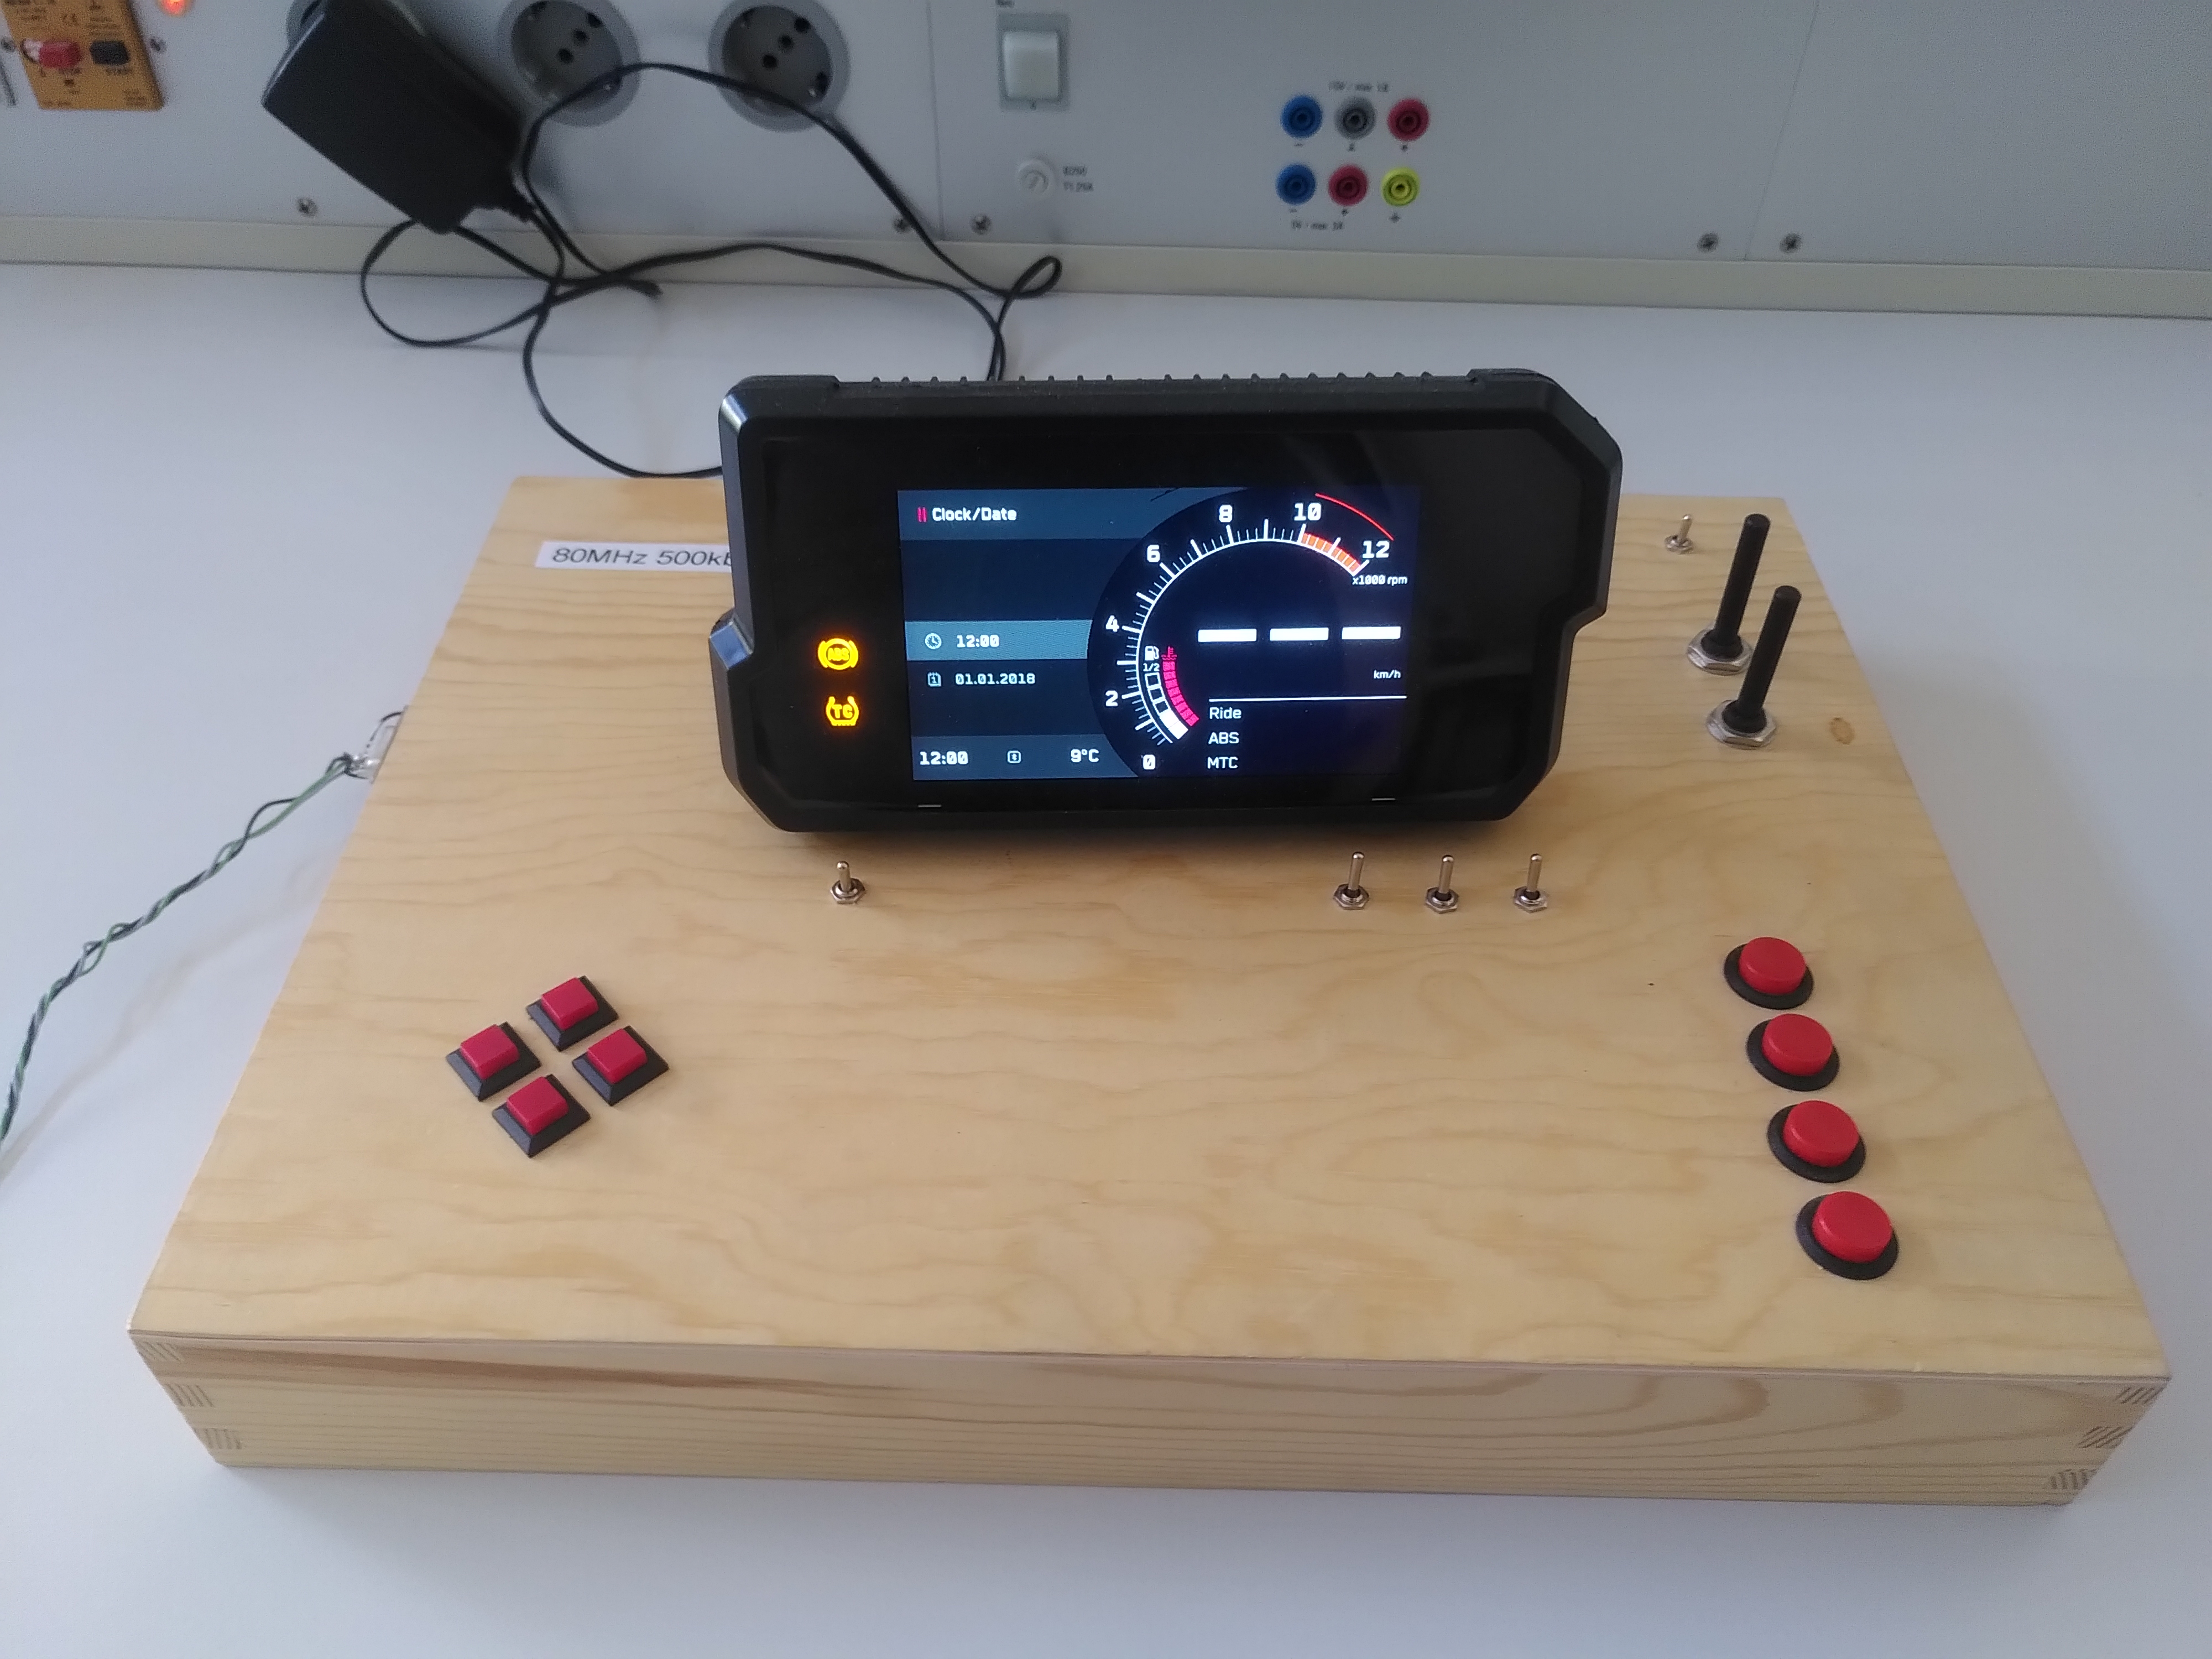
\includegraphics[width=.8\linewidth]{img/demonstration1/ktm_dashboard.jpg}
        \caption{The KTM Dashboard in its sandboxed form.}
    \end{center}
\end{figure}

\subsubsection{Vector}

Vector is a manufacturer of software as well as hardware tools specialised in offering products for the automotive-, transport-, aeronautics and medical industry. Founded in 1988 in Stuttgart, their products are used worldwide for calibration, testing and diagnosis of many different systems. %TODO cite https://www.vector.com/de/de/

One area of particular focus for the company are tools interacting with the CAN bus. Their VN1600 family of bus interfaces offers many solutions for directly plugging into the CAN sockets of a system that uses such a bus and allow a user to send packets. For this demonstration a VN1610 CAN interface was used in order to allow a computer running Windows 10 to execute a python script that sends CAN packets to the bus. %TODO https://cdn.vector.com/cms/content/products/VN16xx/docs/VN16xx_FactSheet_DE.pdf

\begin{figure}[!h]
    \begin{center}
        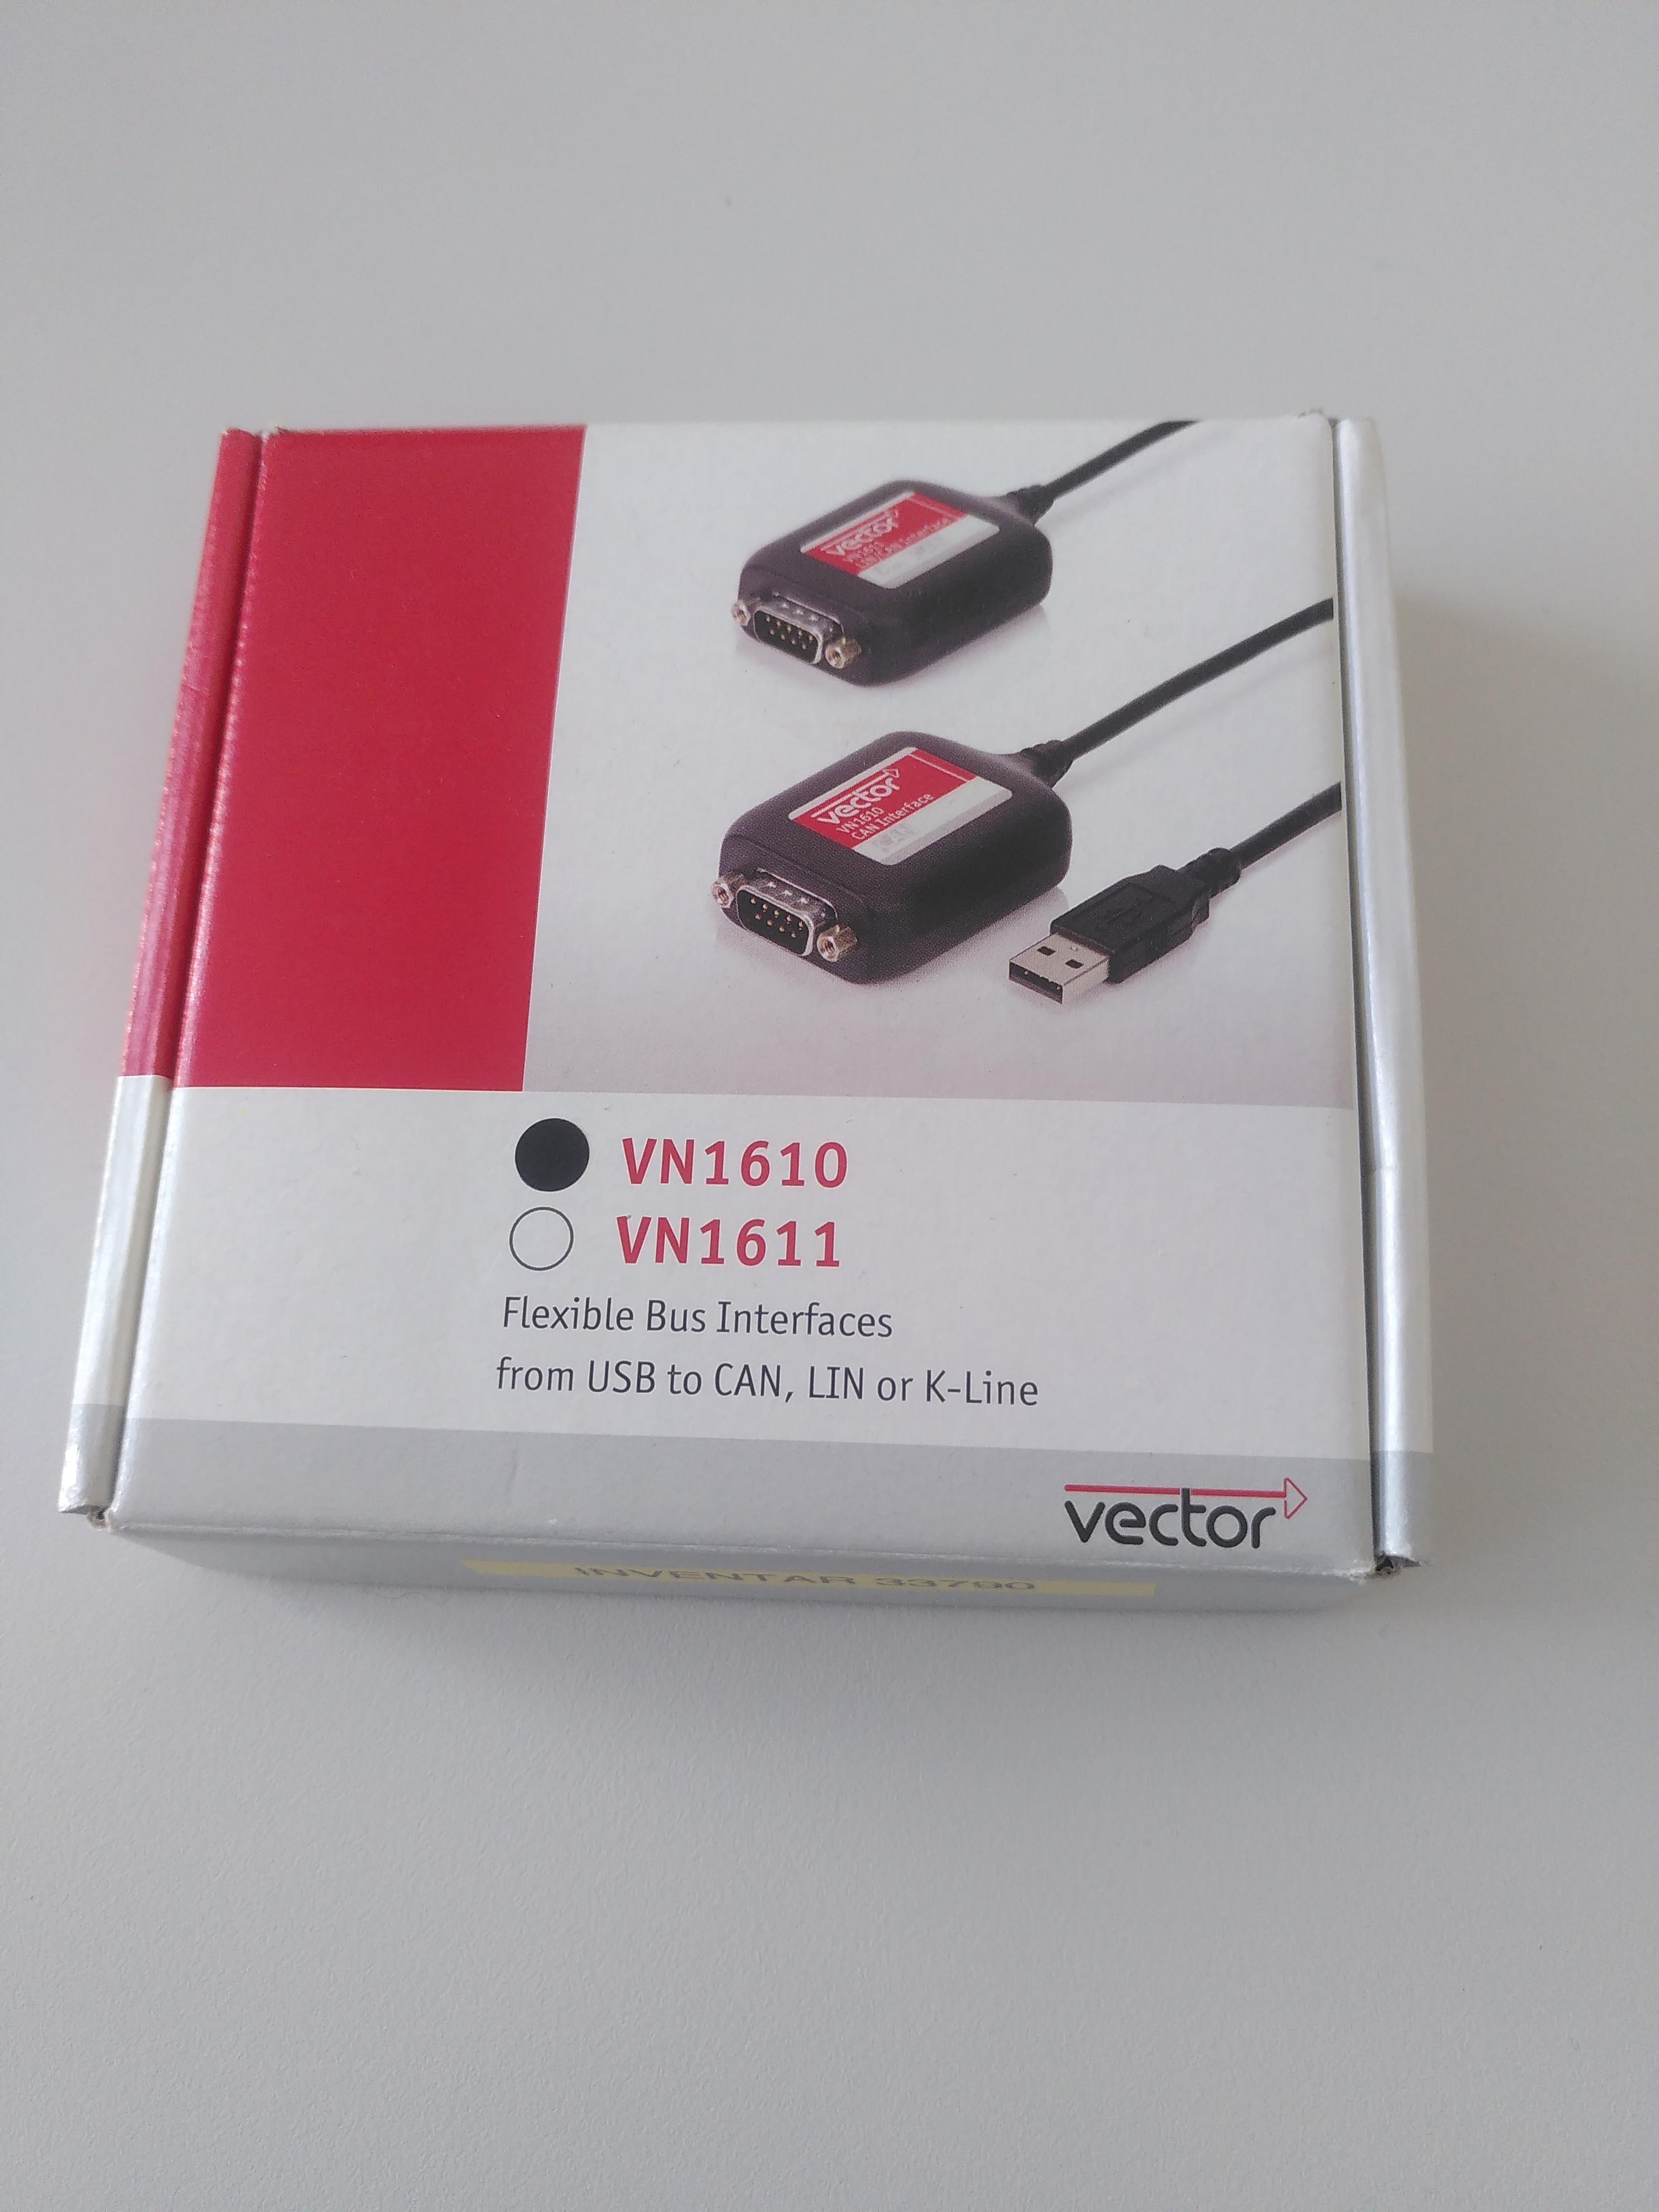
\includegraphics[width=.6\linewidth]{img/demonstration1/vector_box.jpg}
        \caption{The Vector VN1610 connector in its box.}
    \end{center}
\end{figure}

Once the Vector VN1610 was connected to the computer via USB and to the CAN bus, the driver for the bus interface need to be installed and the correct properties of the bus need to be selected.

The ``Vector XL driver library'' can be downloaded and installed from the official vector website. It constitutes of a simple install wizard that can be followed step by step and will not be detailed further here.
%TODO cite https://www.vector.com/int/en/products/products-a-z/libraries-drivers/xl-driver-library/#c75493
\begin{figure}[!h]
    \begin{center}
        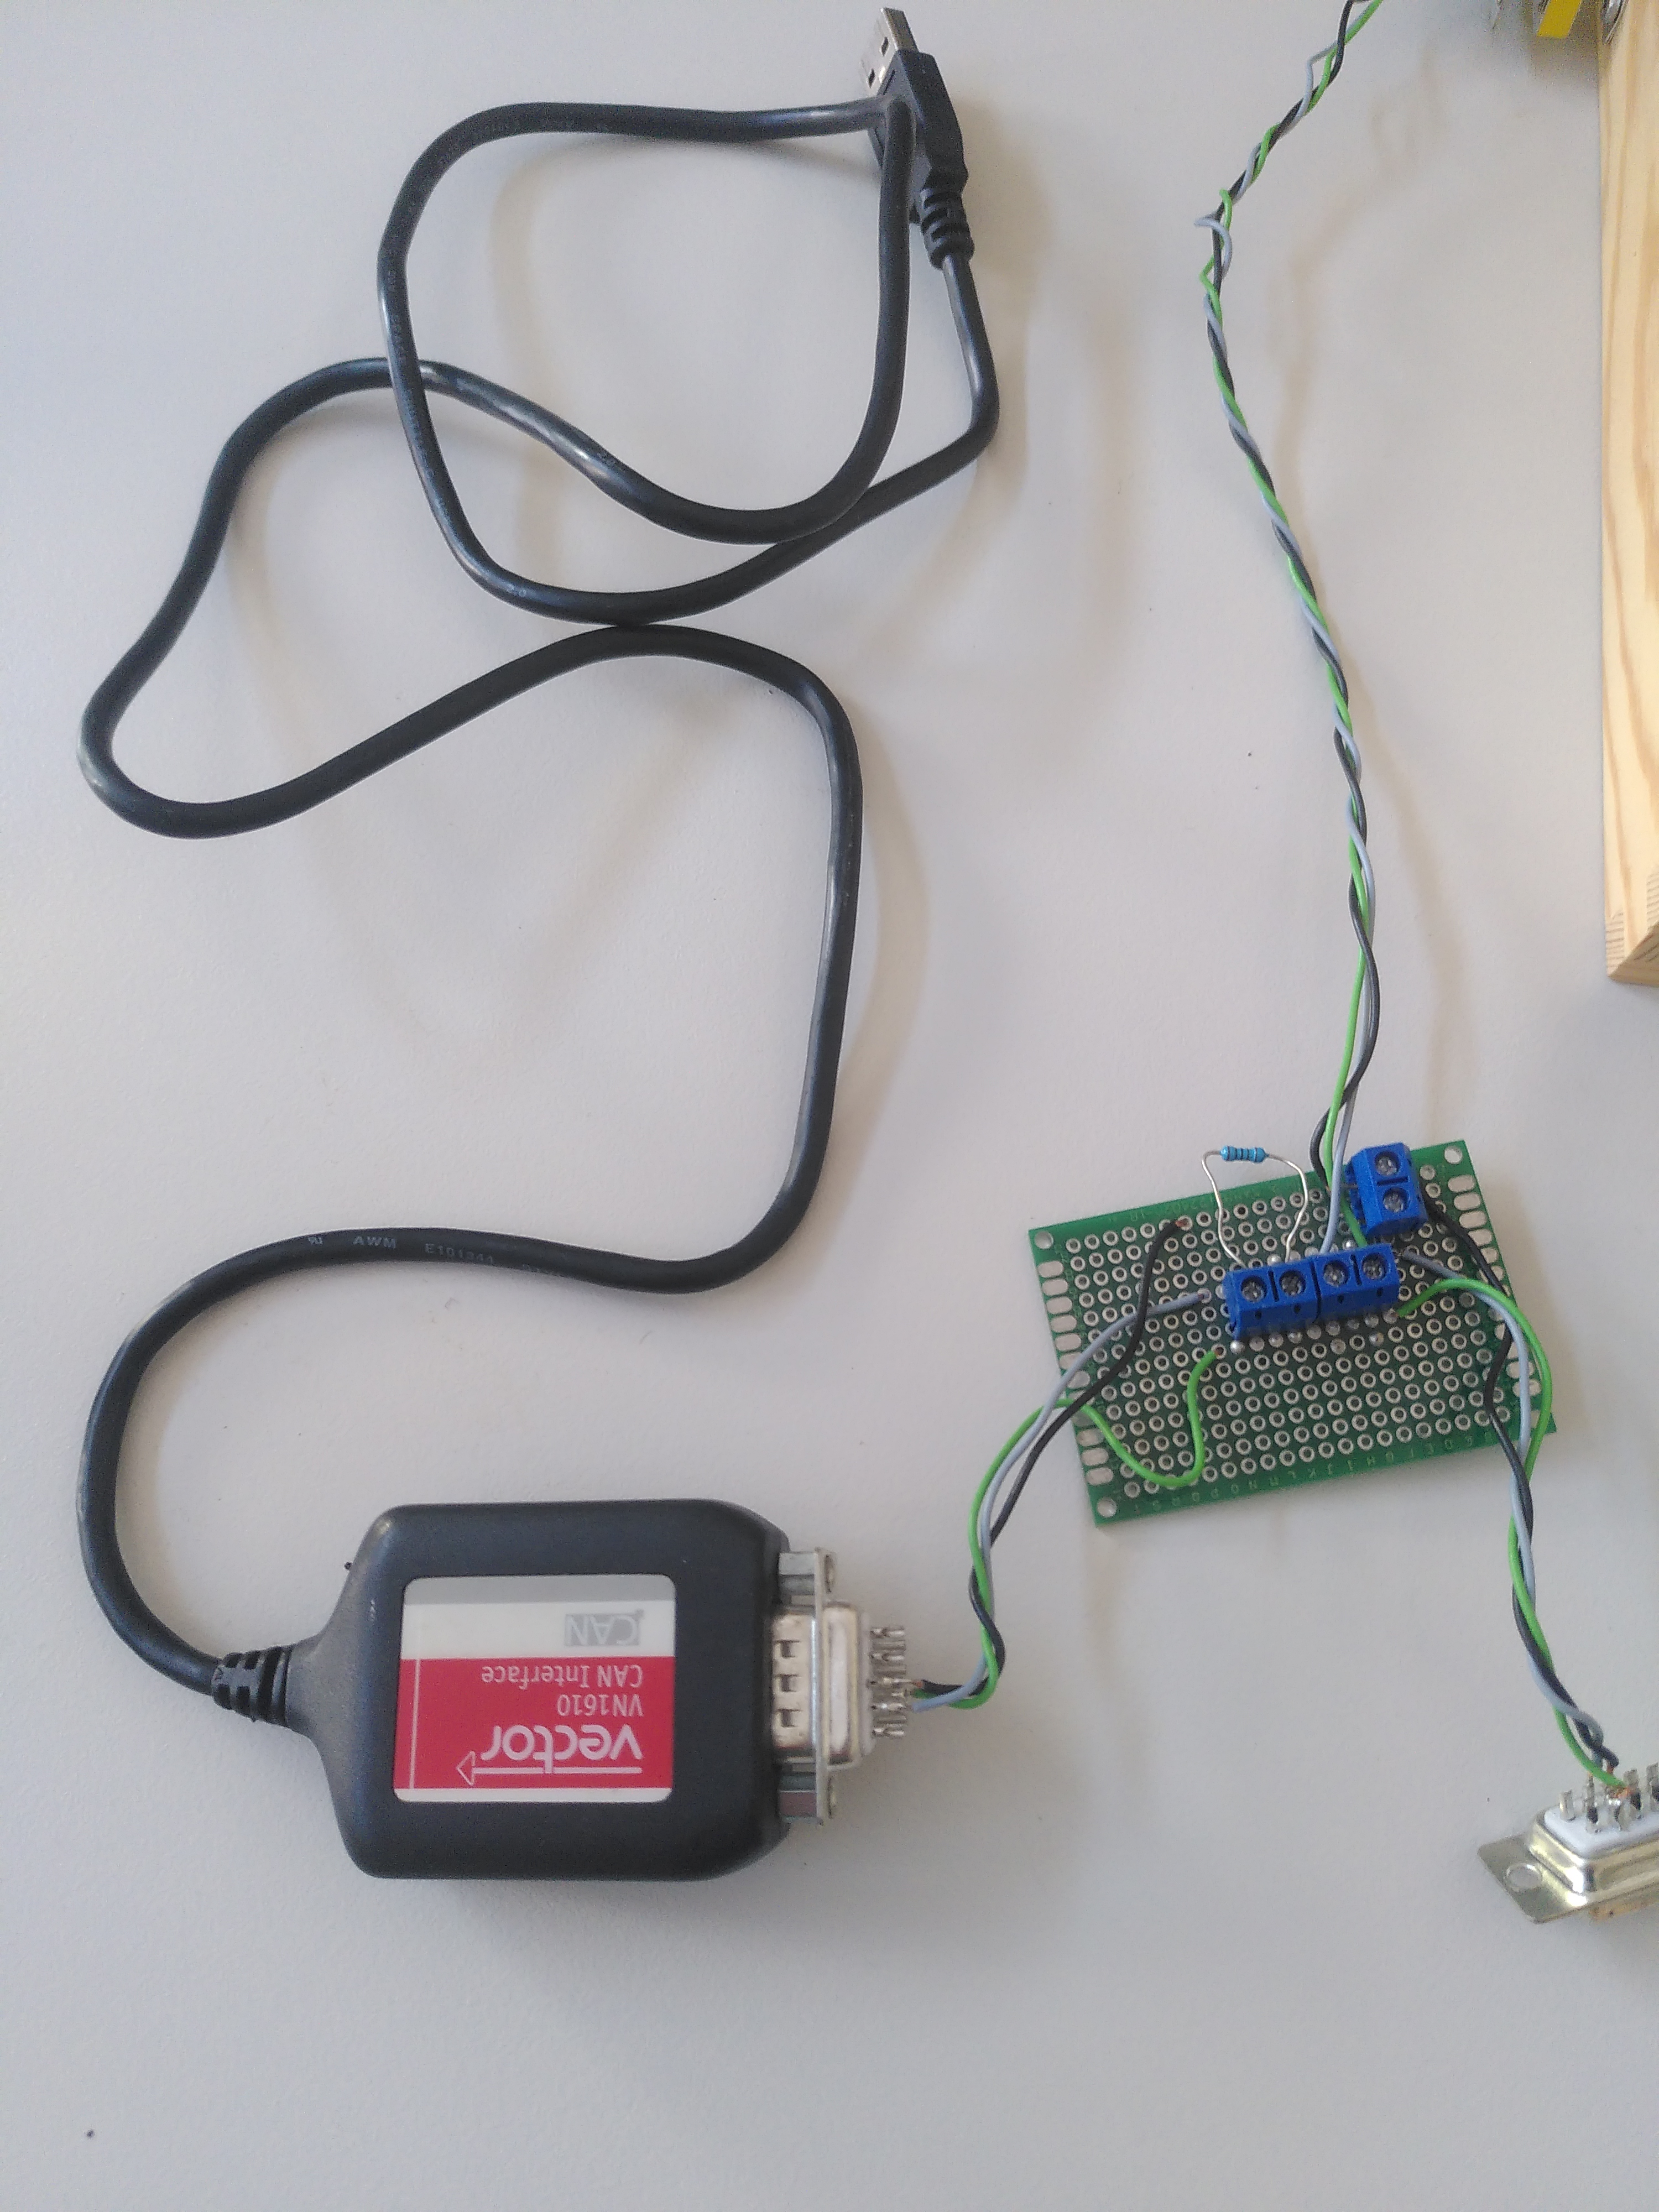
\includegraphics[width=.6\linewidth]{img/demonstration1/vector.jpg}
        \caption{The Vector XL Driver Library Installation Wizard.}
    \end{center}
\end{figure}

After installing the driver, the ``Vector Hardware Manager'' can be executed in order to configure the VN1610 interface. When the program is launched and the VN1610 is connected, a tooltip will show that the device was detected and can be added to the setup. After clicking ``Add to configuration'' and ``Deploy'', the device will be ready to use.

\begin{figure}[!h]
    \begin{center}
        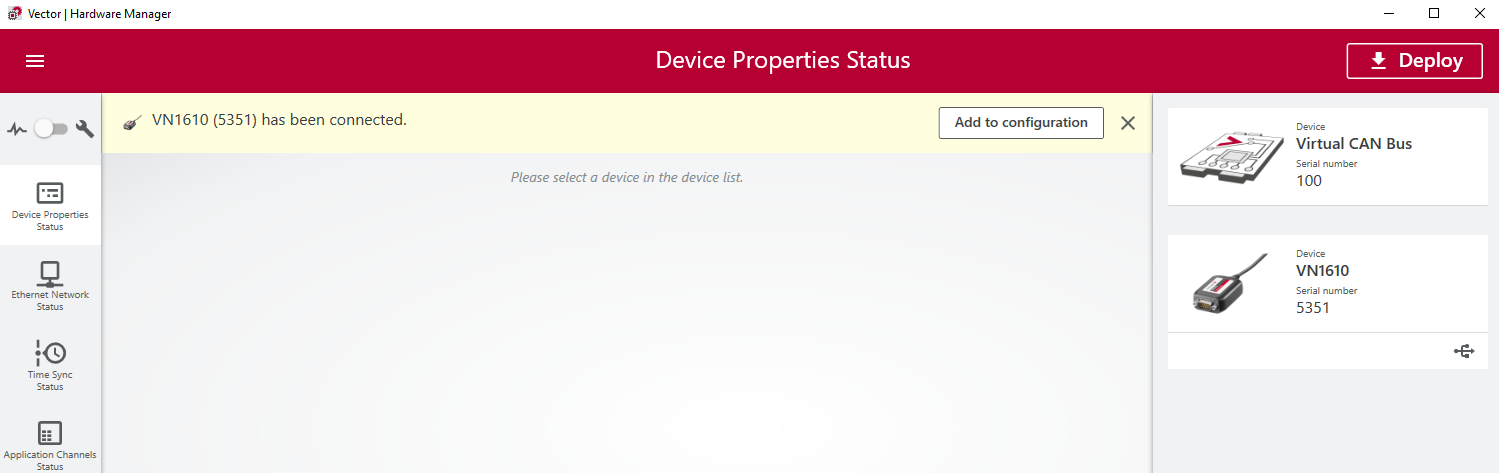
\includegraphics[width=.6\linewidth]{img/demonstration1/vector_hardwaremanager.PNG}
        \caption{The Vector Hardware Manager after connecting the VN1610 via USB.}
    \end{center}
\end{figure}

\begin{figure}[!h]
    \begin{center}
        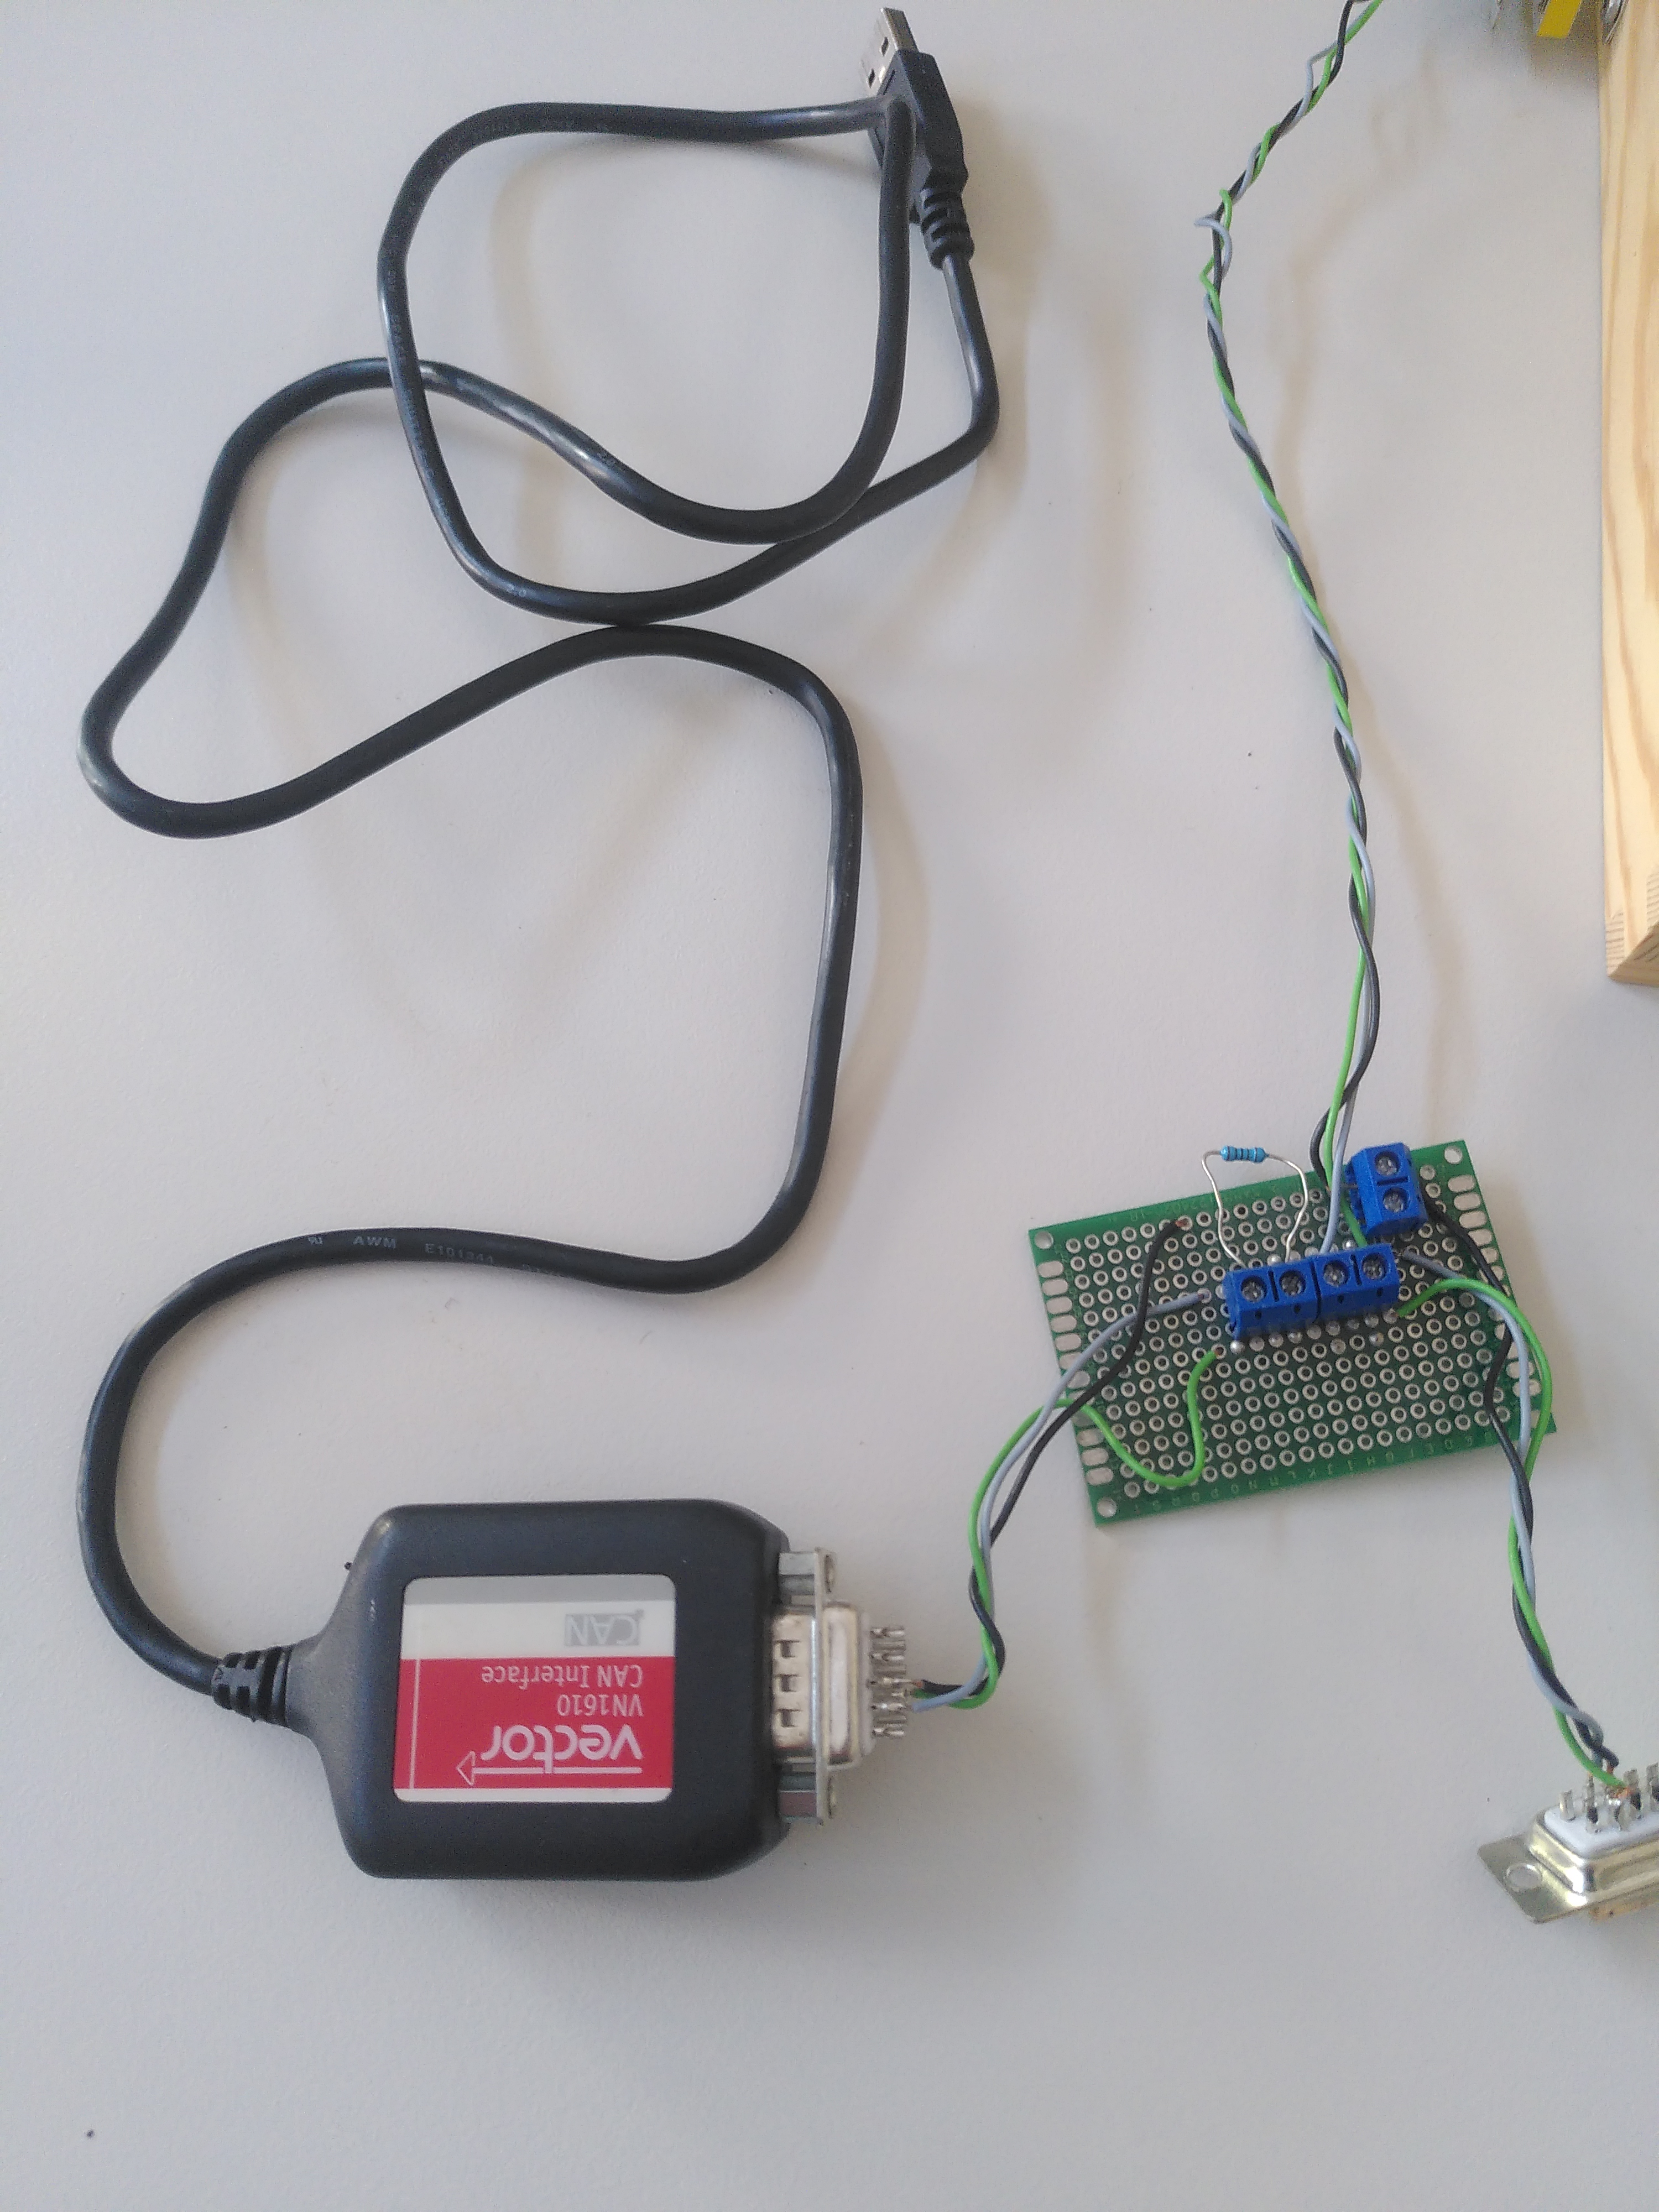
\includegraphics[width=.6\linewidth]{img/demonstration1/vector.jpg}
        \caption{The Vector VN1610 connector attached to the CAN Bus on the KTM dashboard.}
    \end{center}
\end{figure}


\subsubsection{python-can}
Ín order to execute the fuzzing attack, the following python script titled ``canfuzz.py'' was written. It is able to connect to the CAN Bus via python-can and then starts one thread that iterates over all CAN-IDs inside a given range and sends random CAN data to each and every one. Another thread meanwhile continually checks for incoming messages on the bus.
\begin{verbatim}
import can
import _thread
import time
import random

# this function takes some data, splits it into 8 bytes
# and sends it adressed to a specific CAN ID
def send_canmessage(bus, canid, candata):
    #split the data into 8 bytes
    b8 = (candata >> 0) & 0xFF
    b7 = (candata >> 8) & 0xFF
    b6 = (candata >> 16) & 0xFF
    b5 = (candata >> 24) & 0xFF
    b4 = (candata >> 32) & 0xFF
    b3 = (candata >> 40) & 0xFF
    b2 = (candata >> 48) & 0xFF
    b1 = (candata >> 56) & 0xFF

    candata_split = [b1, b2, b3, b4, b5, b6, b7, b8]

    #debug output
    #print(f"sending Message {message} on {hex(canid)}")

    #message consists of ID, data and extended can flag
    message = can.Message(
        arbitration_id = canid, 
        data = candata_split, 
        is_extended_id = False
    )

    #try to send the message and sleep for a bit
    try:
        bus.send(message)
        time.sleep(0.05)
    except can.CanError:
        #most likely the queue is full, so wait a little
        #longer and then try again
        print("cue was probably full")
        time.sleep(1)
        bus.send(msg)


def sender_thread(bus):
    #iterate over a
    #note that for the dashboard most communication occurs
    #for the IDs 0x450, 0x451, 0x551 and 0x552
    #thats we we can limit the loop to this range
    for canid in range(0x450, 0x560):
        send_canmessage(
            bus, 
            canid, 
            random.randrange(0xFFFFFFFFFFFFFFFF)
        )


def listener_thread(bus):
    #create a listener/printer object
    print_listener = can.Printer()
    #constantly listen for CAN messages and print them
    while(1<2):
        msg = bus.recv()
        print_listener.on_message_received(msg)
    #this point is never reached
    listener.stop()


if __name__ == "__main__":
    # establish can bus connection, listen for own messages
    with can.Bus(receive_own_messages=True) as bus:

        #start thread to listen for CAN message
        _thread.start_new_thread(listener_thread, (bus,))

        #start thread to send CAN messages
        _thread.start_new_thread(sender_thread, (bus,))

        #this is just to keep main function busy
        while(1<2):
            pass
\end{verbatim}

\subsubsection{Result}
The script can be run with the following command (assuming Python 3 is installed on the system):
\begin{verbatim}
python3 canfuzz.py
\end{verbatim}

During execution, the console output looks as follows. It continually prints messages transmitted on the CAN bus. Incoming messages are marked as `RX', while outgoing messages (generated by the script) are marked `TX'. Here it is apparent, that all outgoing messages iterate over CAN IDs within the given range and send random data.

\begin{figure}[!h]
    \begin{center}
        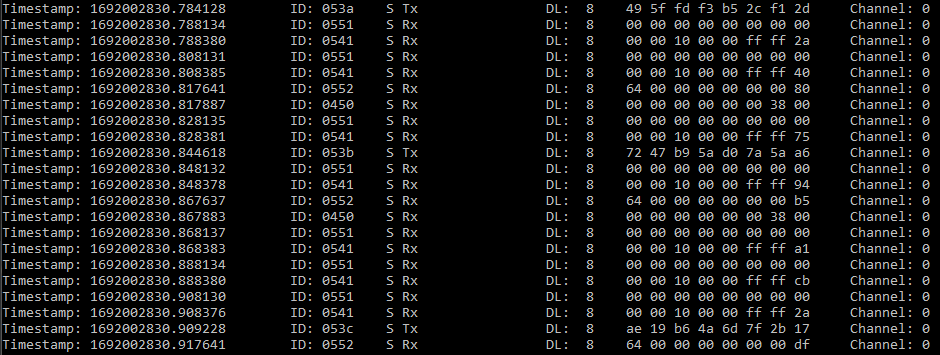
\includegraphics[width=.6\linewidth]{img/demonstration1/console_output_cropped.PNG}
        \caption{The console output while running canfuzz.py.}
    \end{center}
\end{figure}

After running the script for a few seconds multiple messages appear on the motorcycle dashboard screen. After multiple runs the CAN messages the script sent were able to influence the following readouts on the device:
\begin{itemize}
	\item Engine Temperature Sensor
	\item Transport Lock
	\item Side Stand Position / Ignition
	\item Oil Temperature
\end{verse}
In addition to manipulating this sensor data, we were also able to produce ECU, Immobilizer Antenna and key failures.

\begin{figure}
	\begin{subfigure}{.5\textwidth}
		\centering
		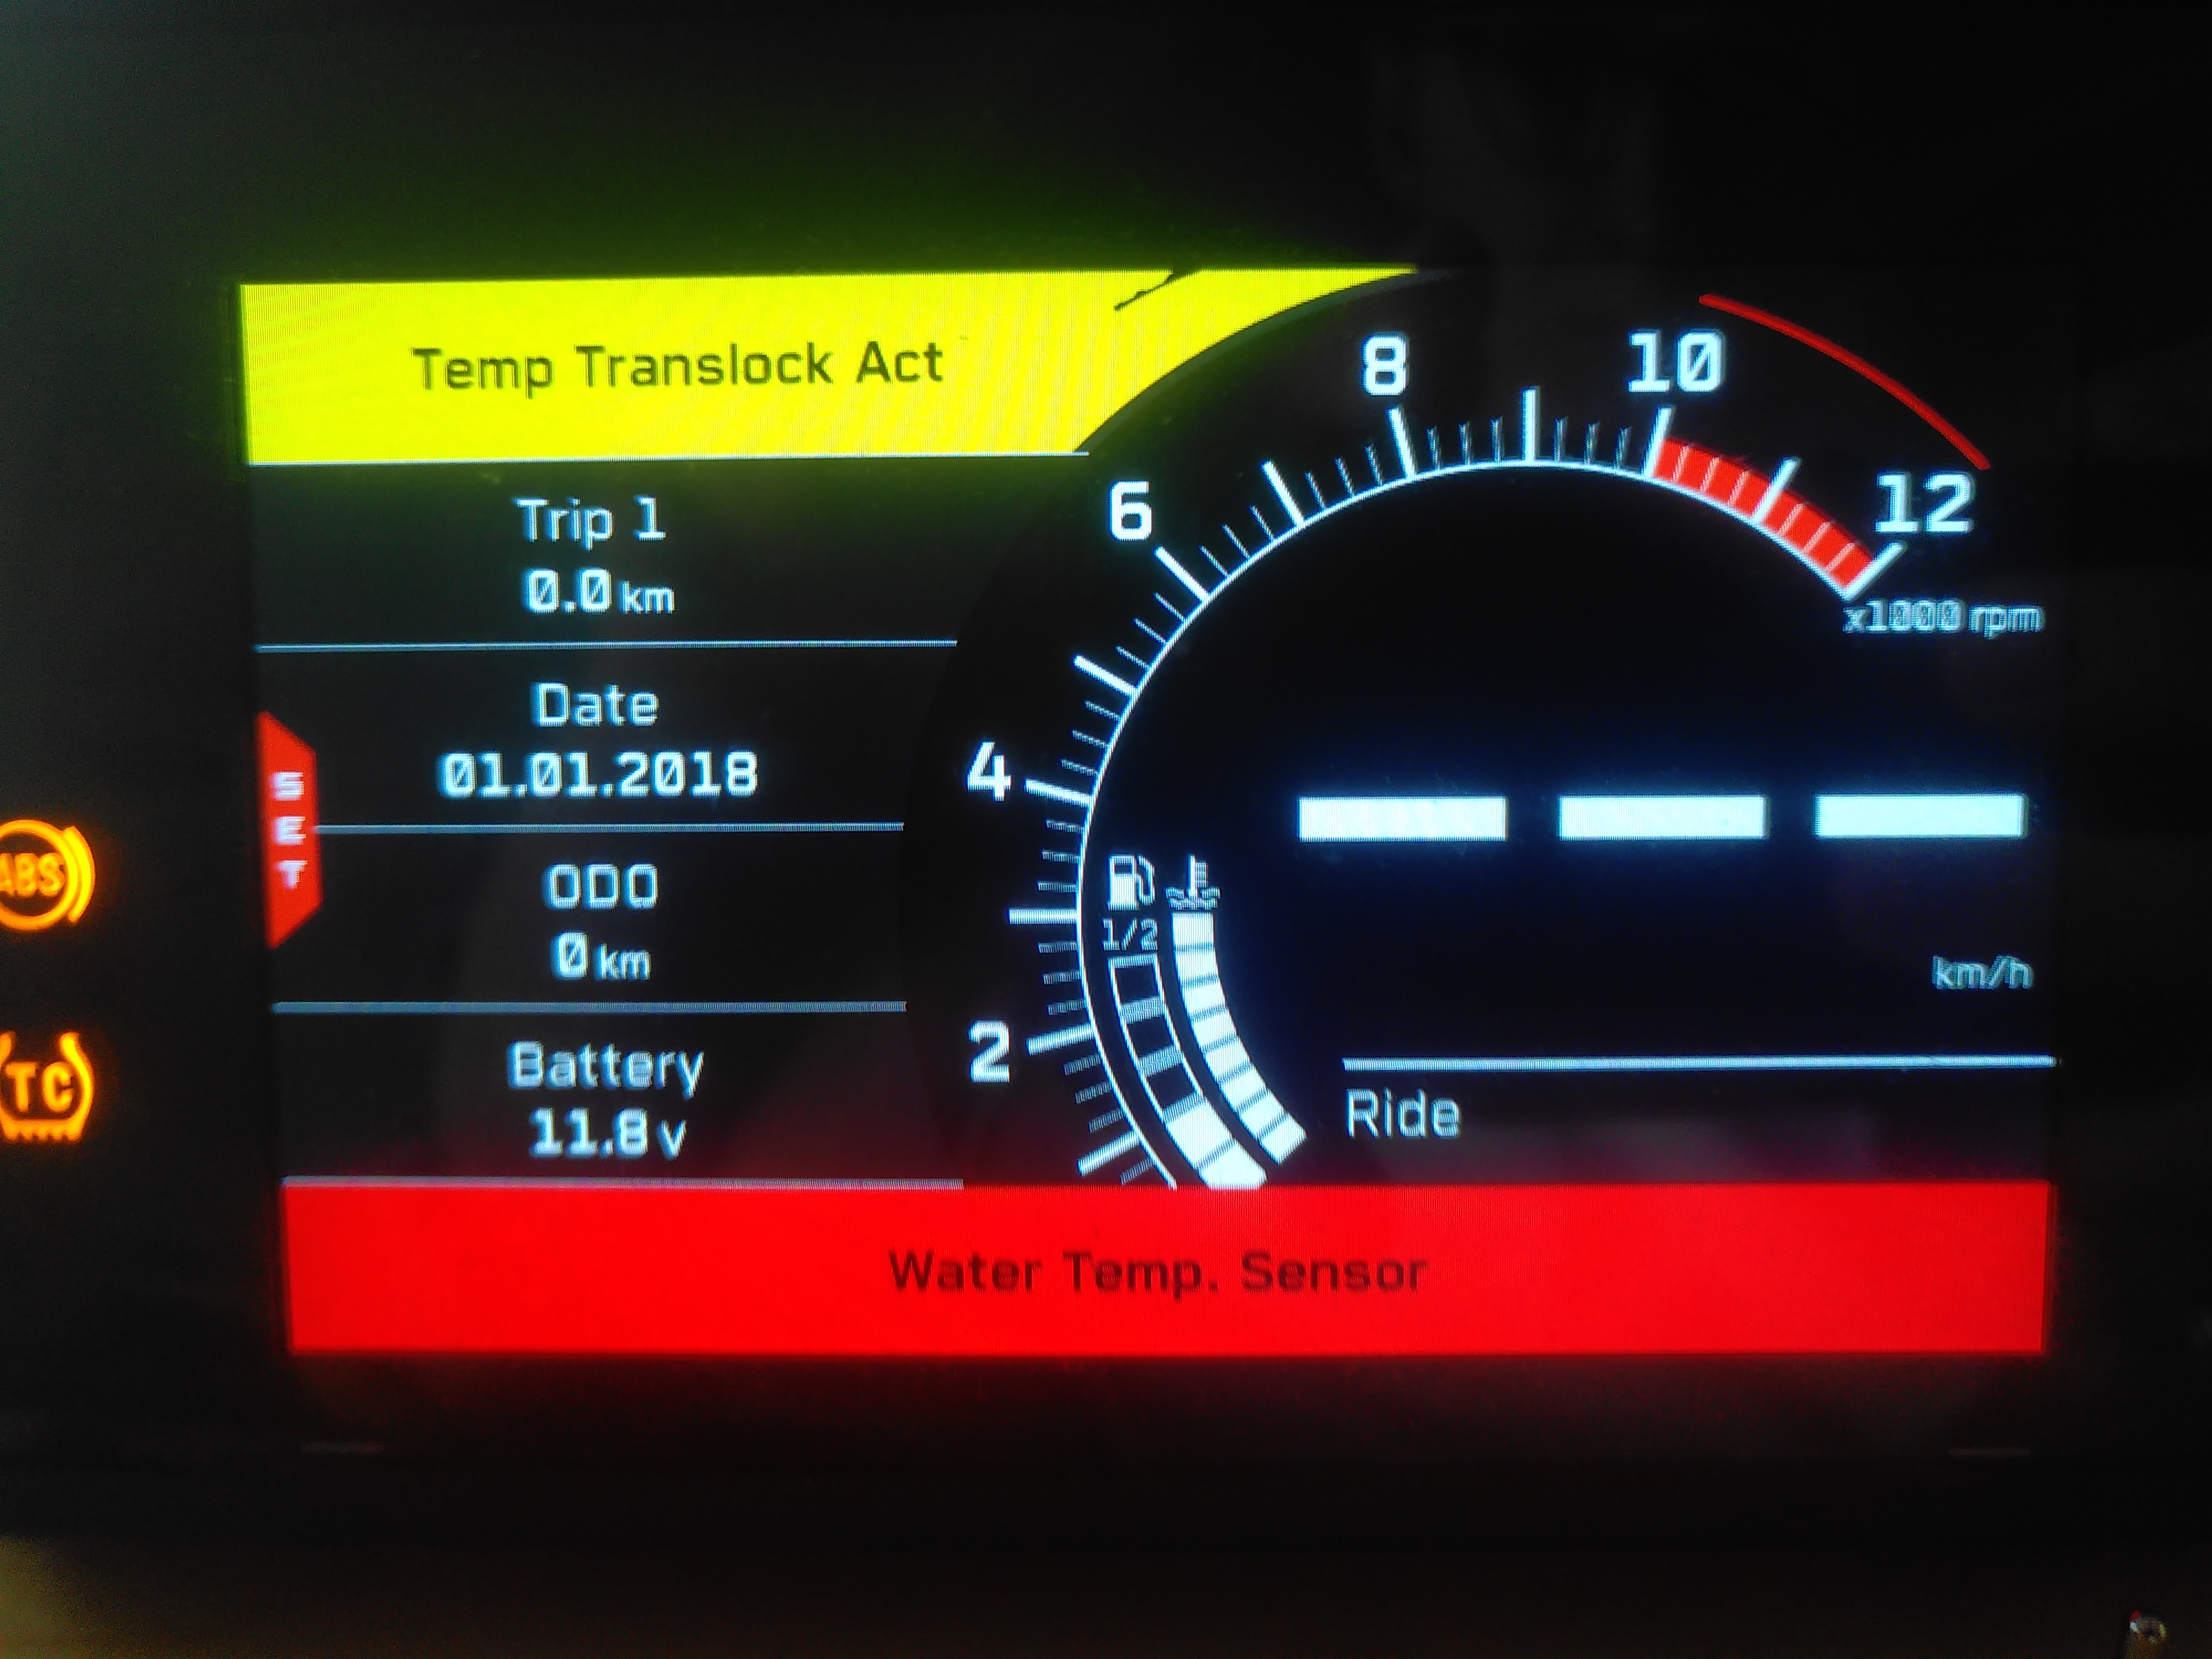
\includegraphics[width=.8\linewidth]{img/demonstration1/result1.jpg}
		\caption{1a}
		\label{fig:sfig1}
	\end{subfigure}%
	\begin{subfigure}{.5\textwidth}
		\centering
		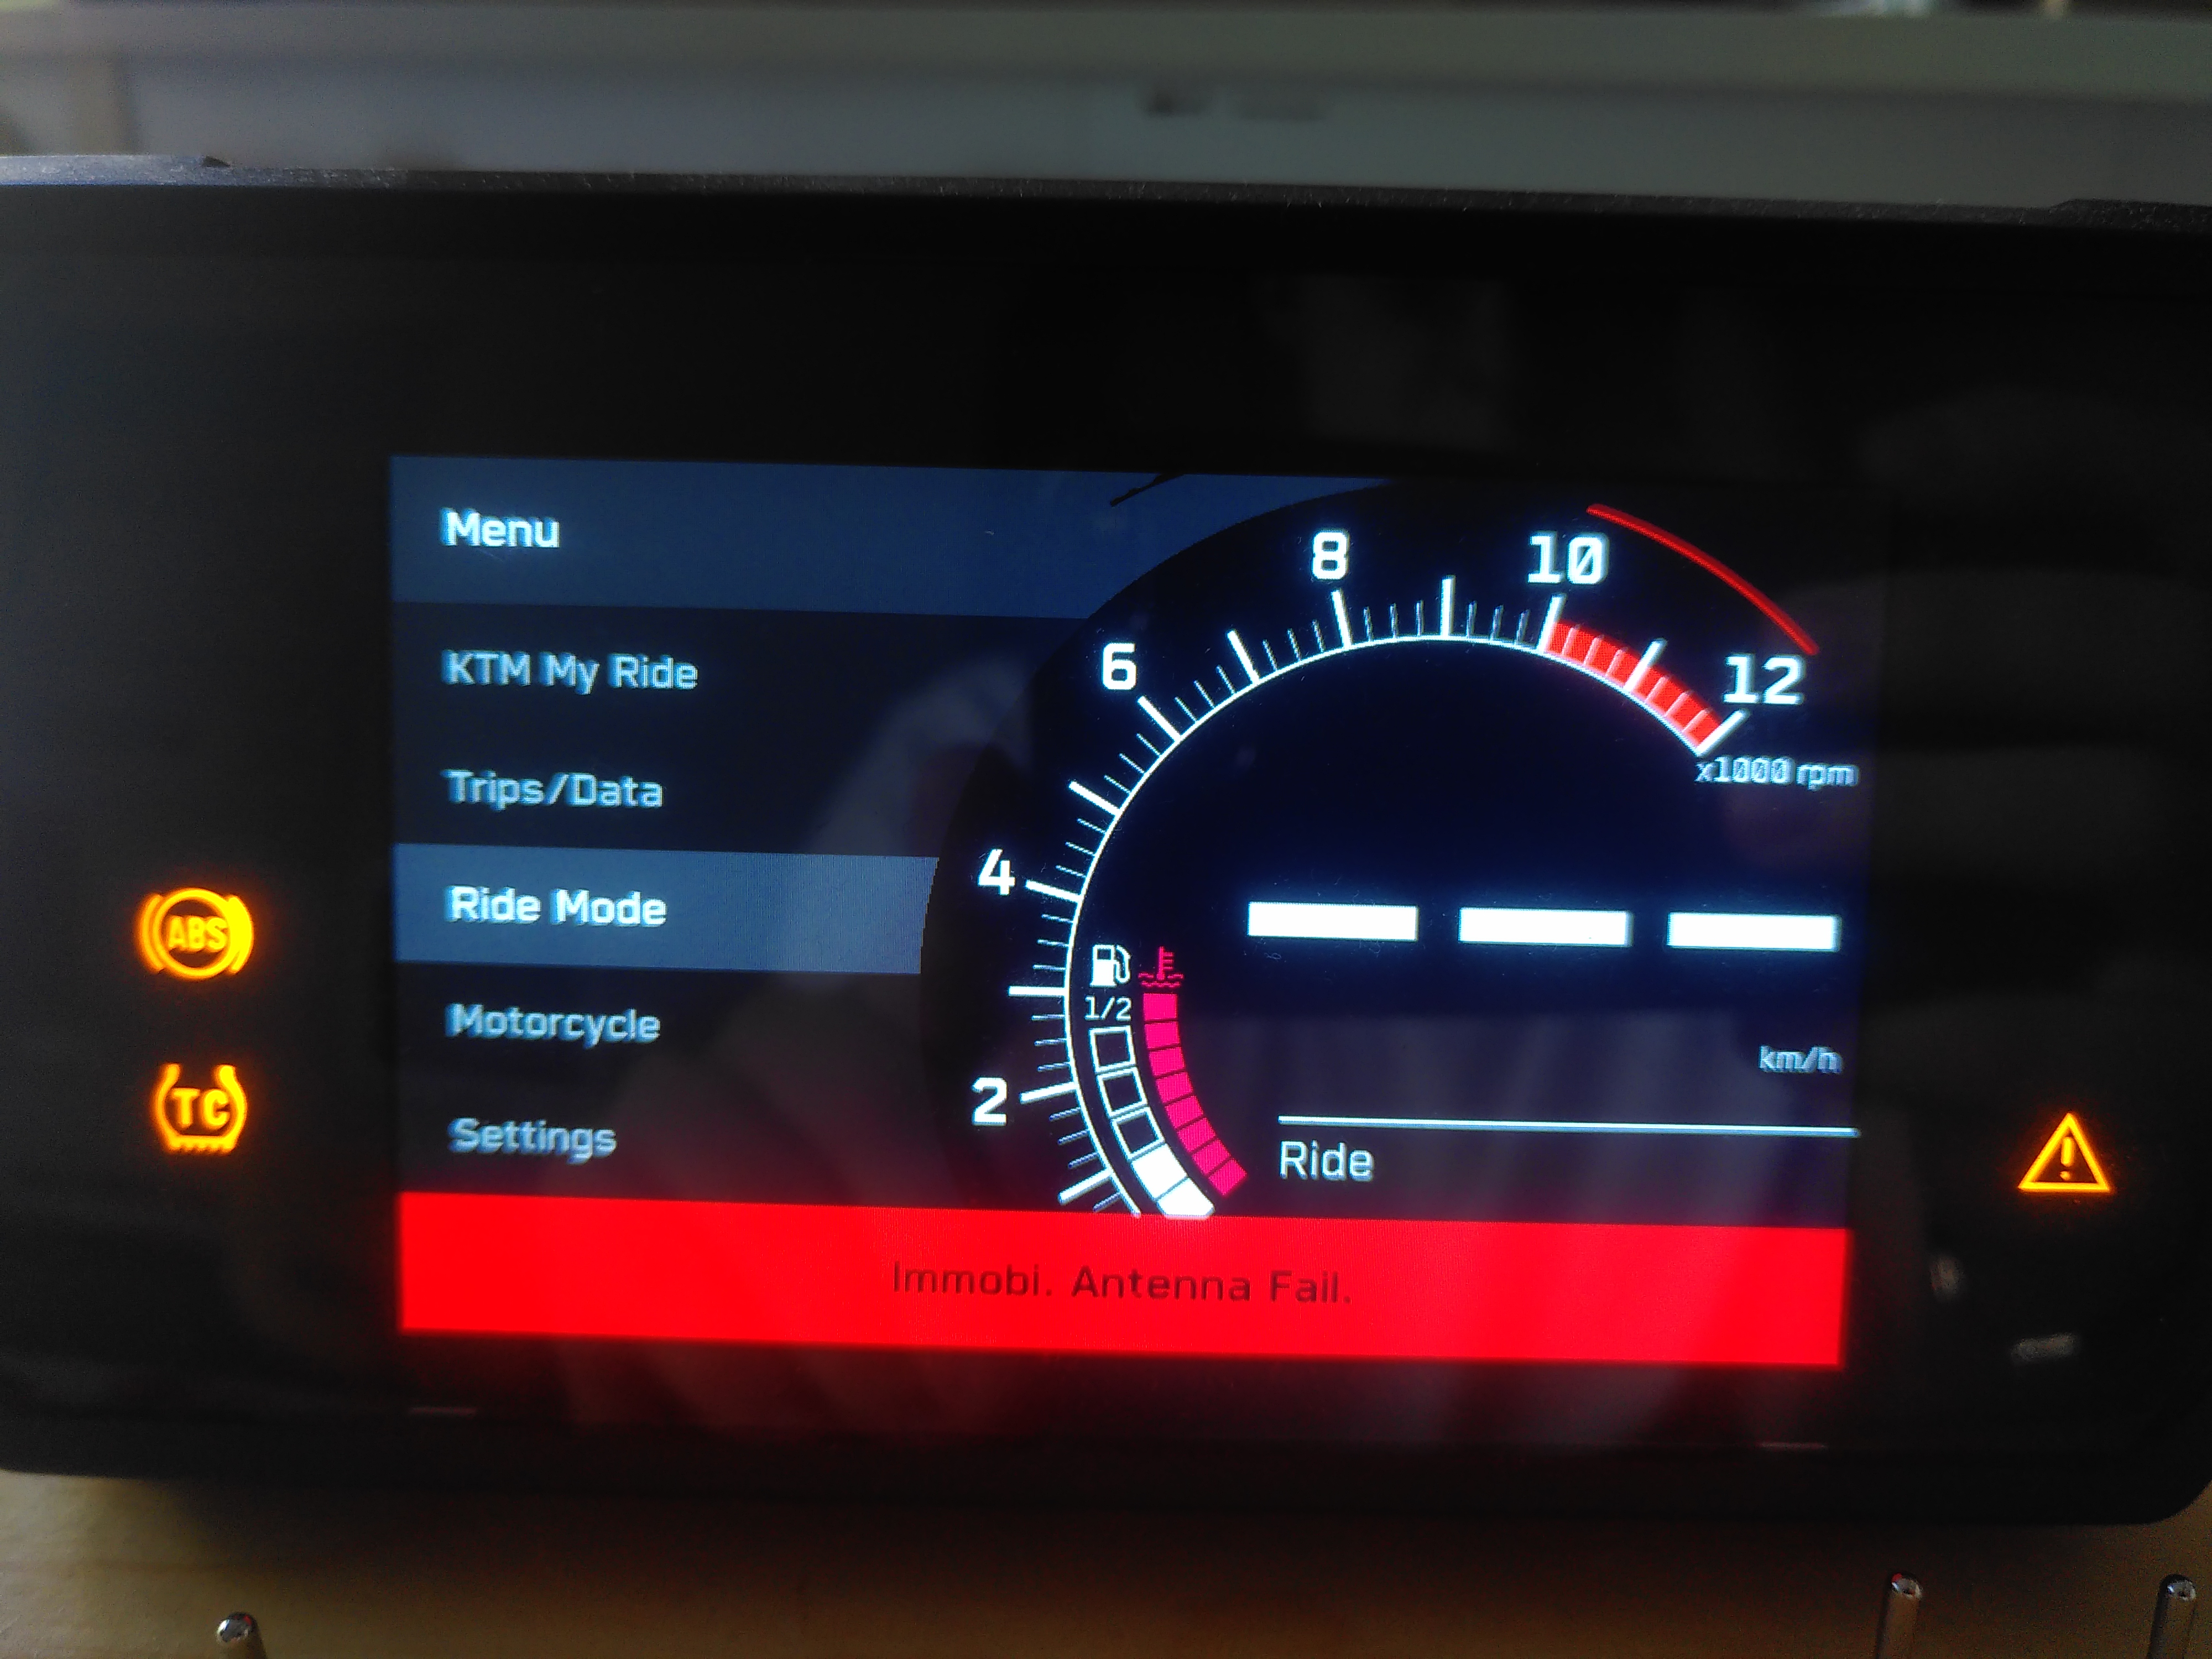
\includegraphics[width=.8\linewidth]{img/demonstration1/result2.jpg}
		\caption{1b}
		\label{fig:sfig2}
	\end{subfigure}
	\caption{plots of....}
	\label{fig:fig}
	\begin{subfigure}{.5\textwidth}
		\centering
		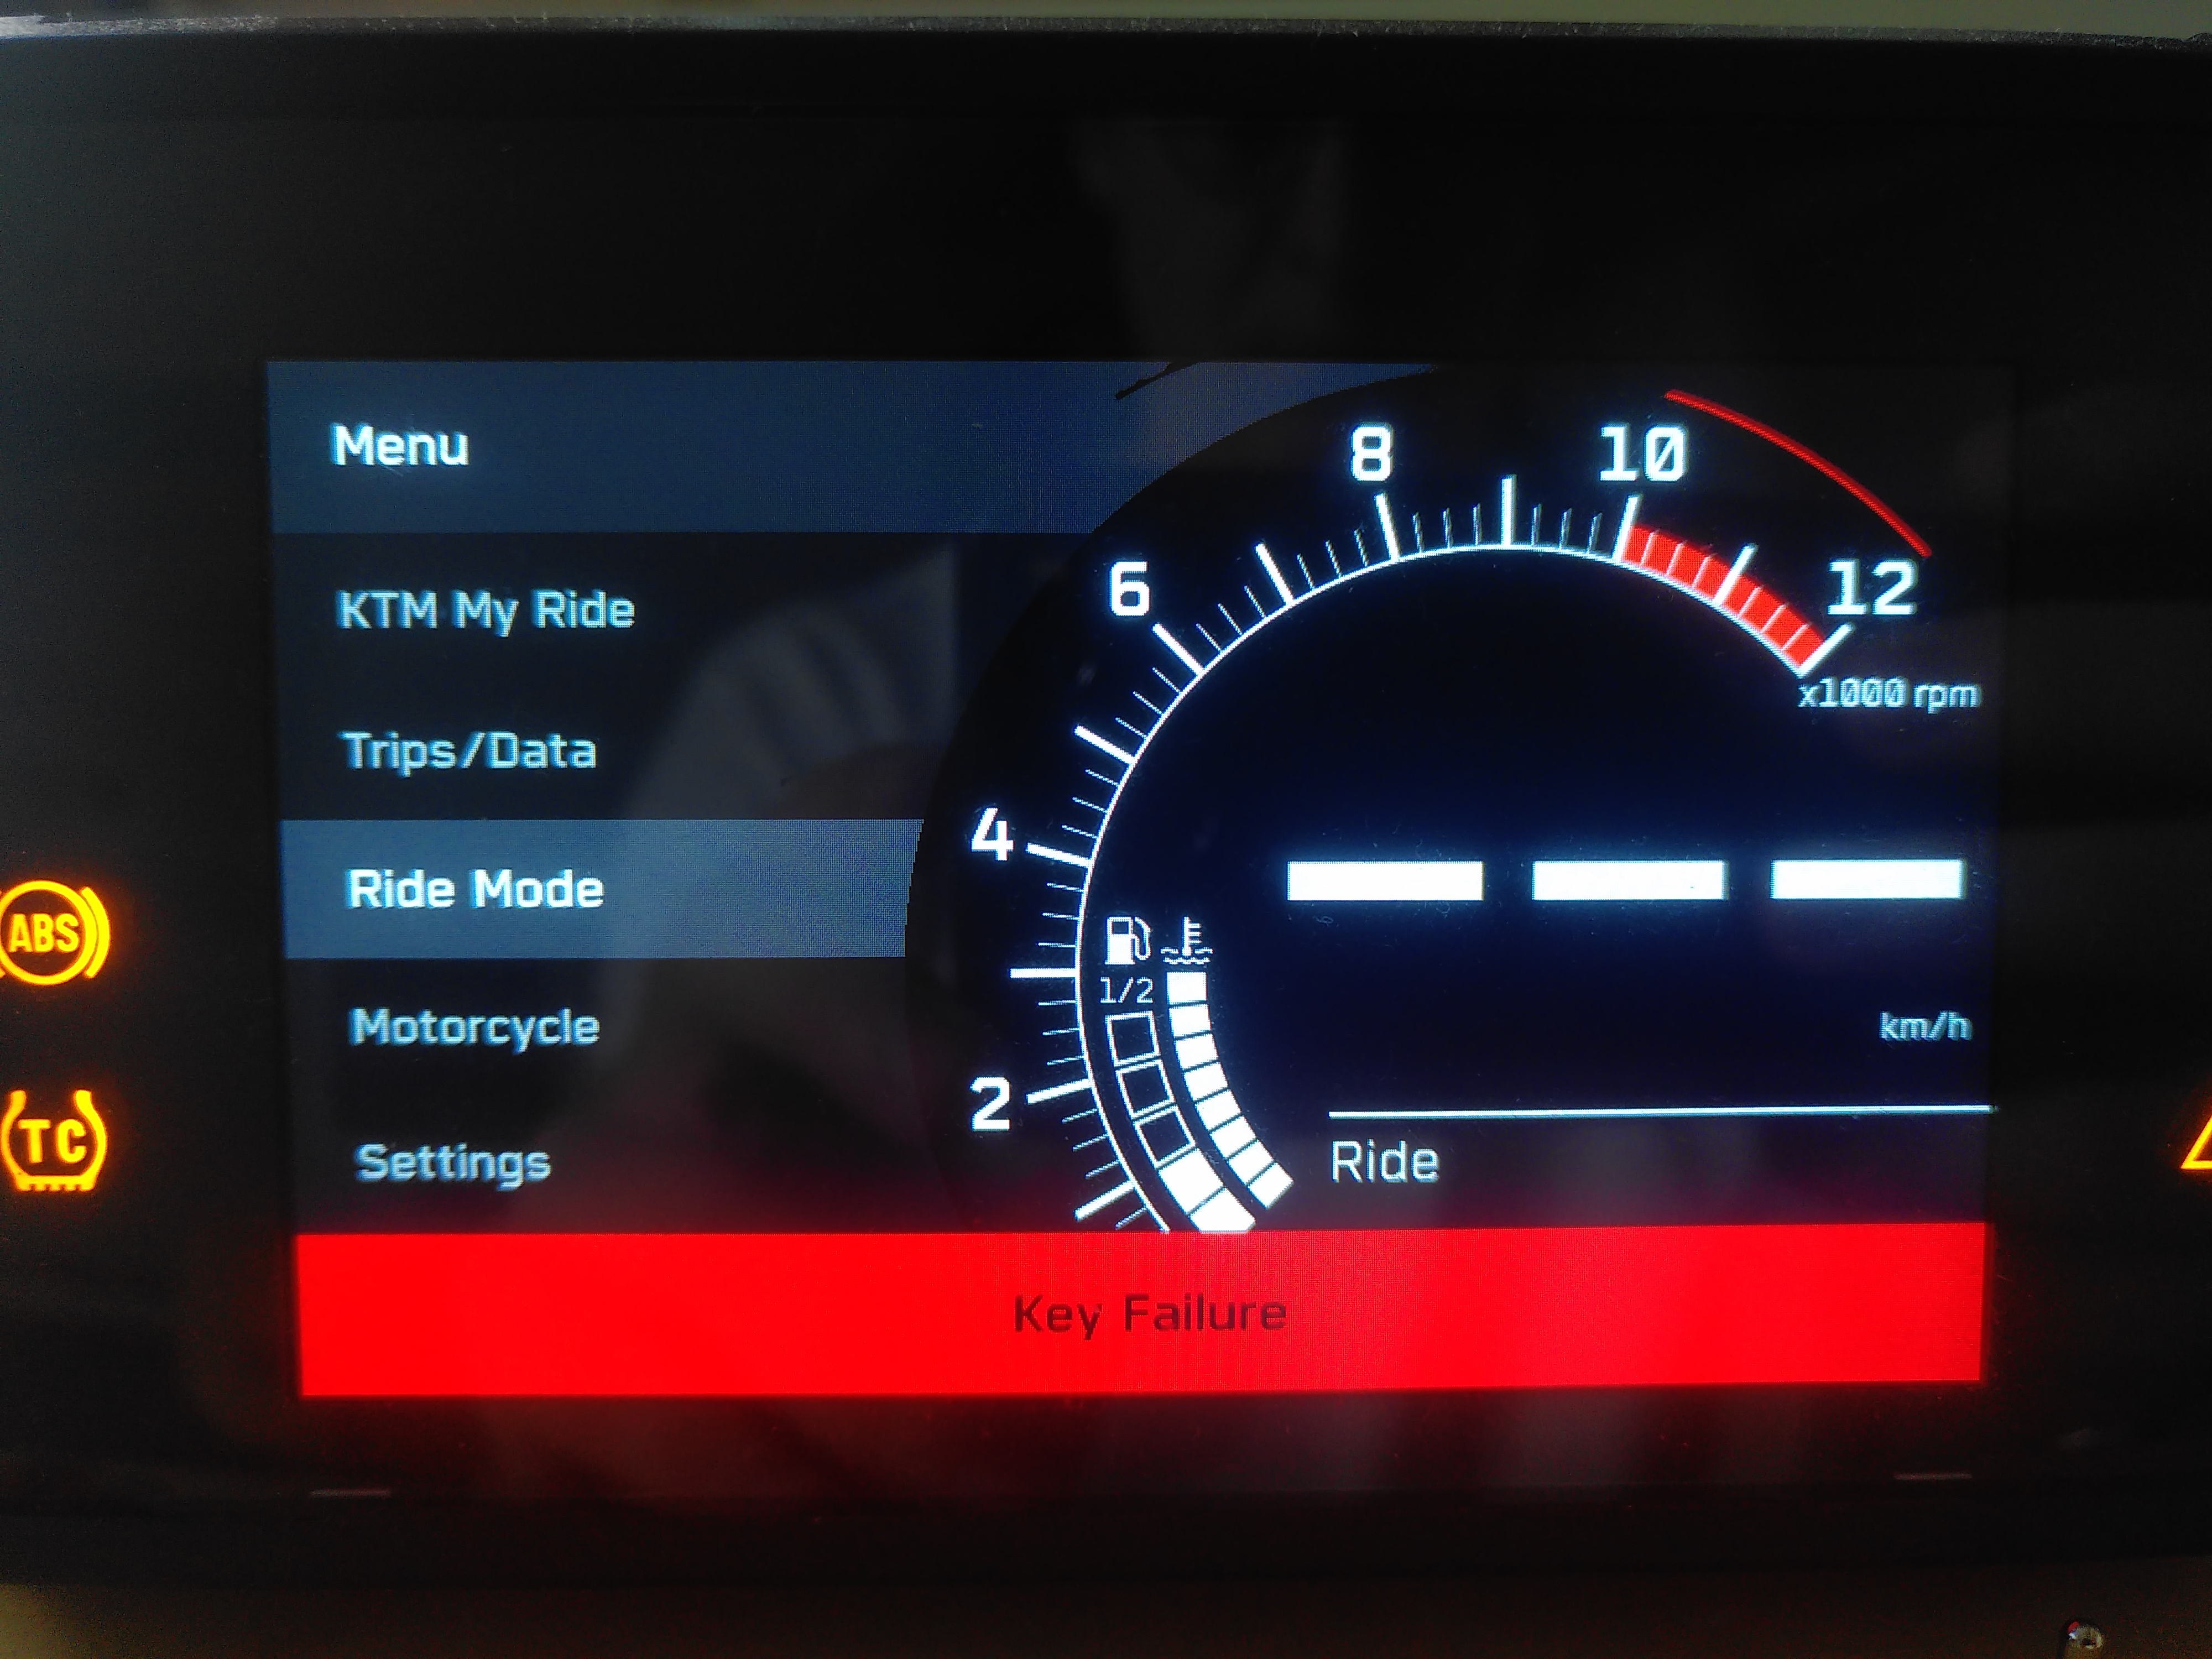
\includegraphics[width=.8\linewidth]{img/demonstration1/result3.jpg}
		\caption{1a}
		\label{fig:sfig1}
	\end{subfigure}%
	\begin{subfigure}{.5\textwidth}
		\centering
		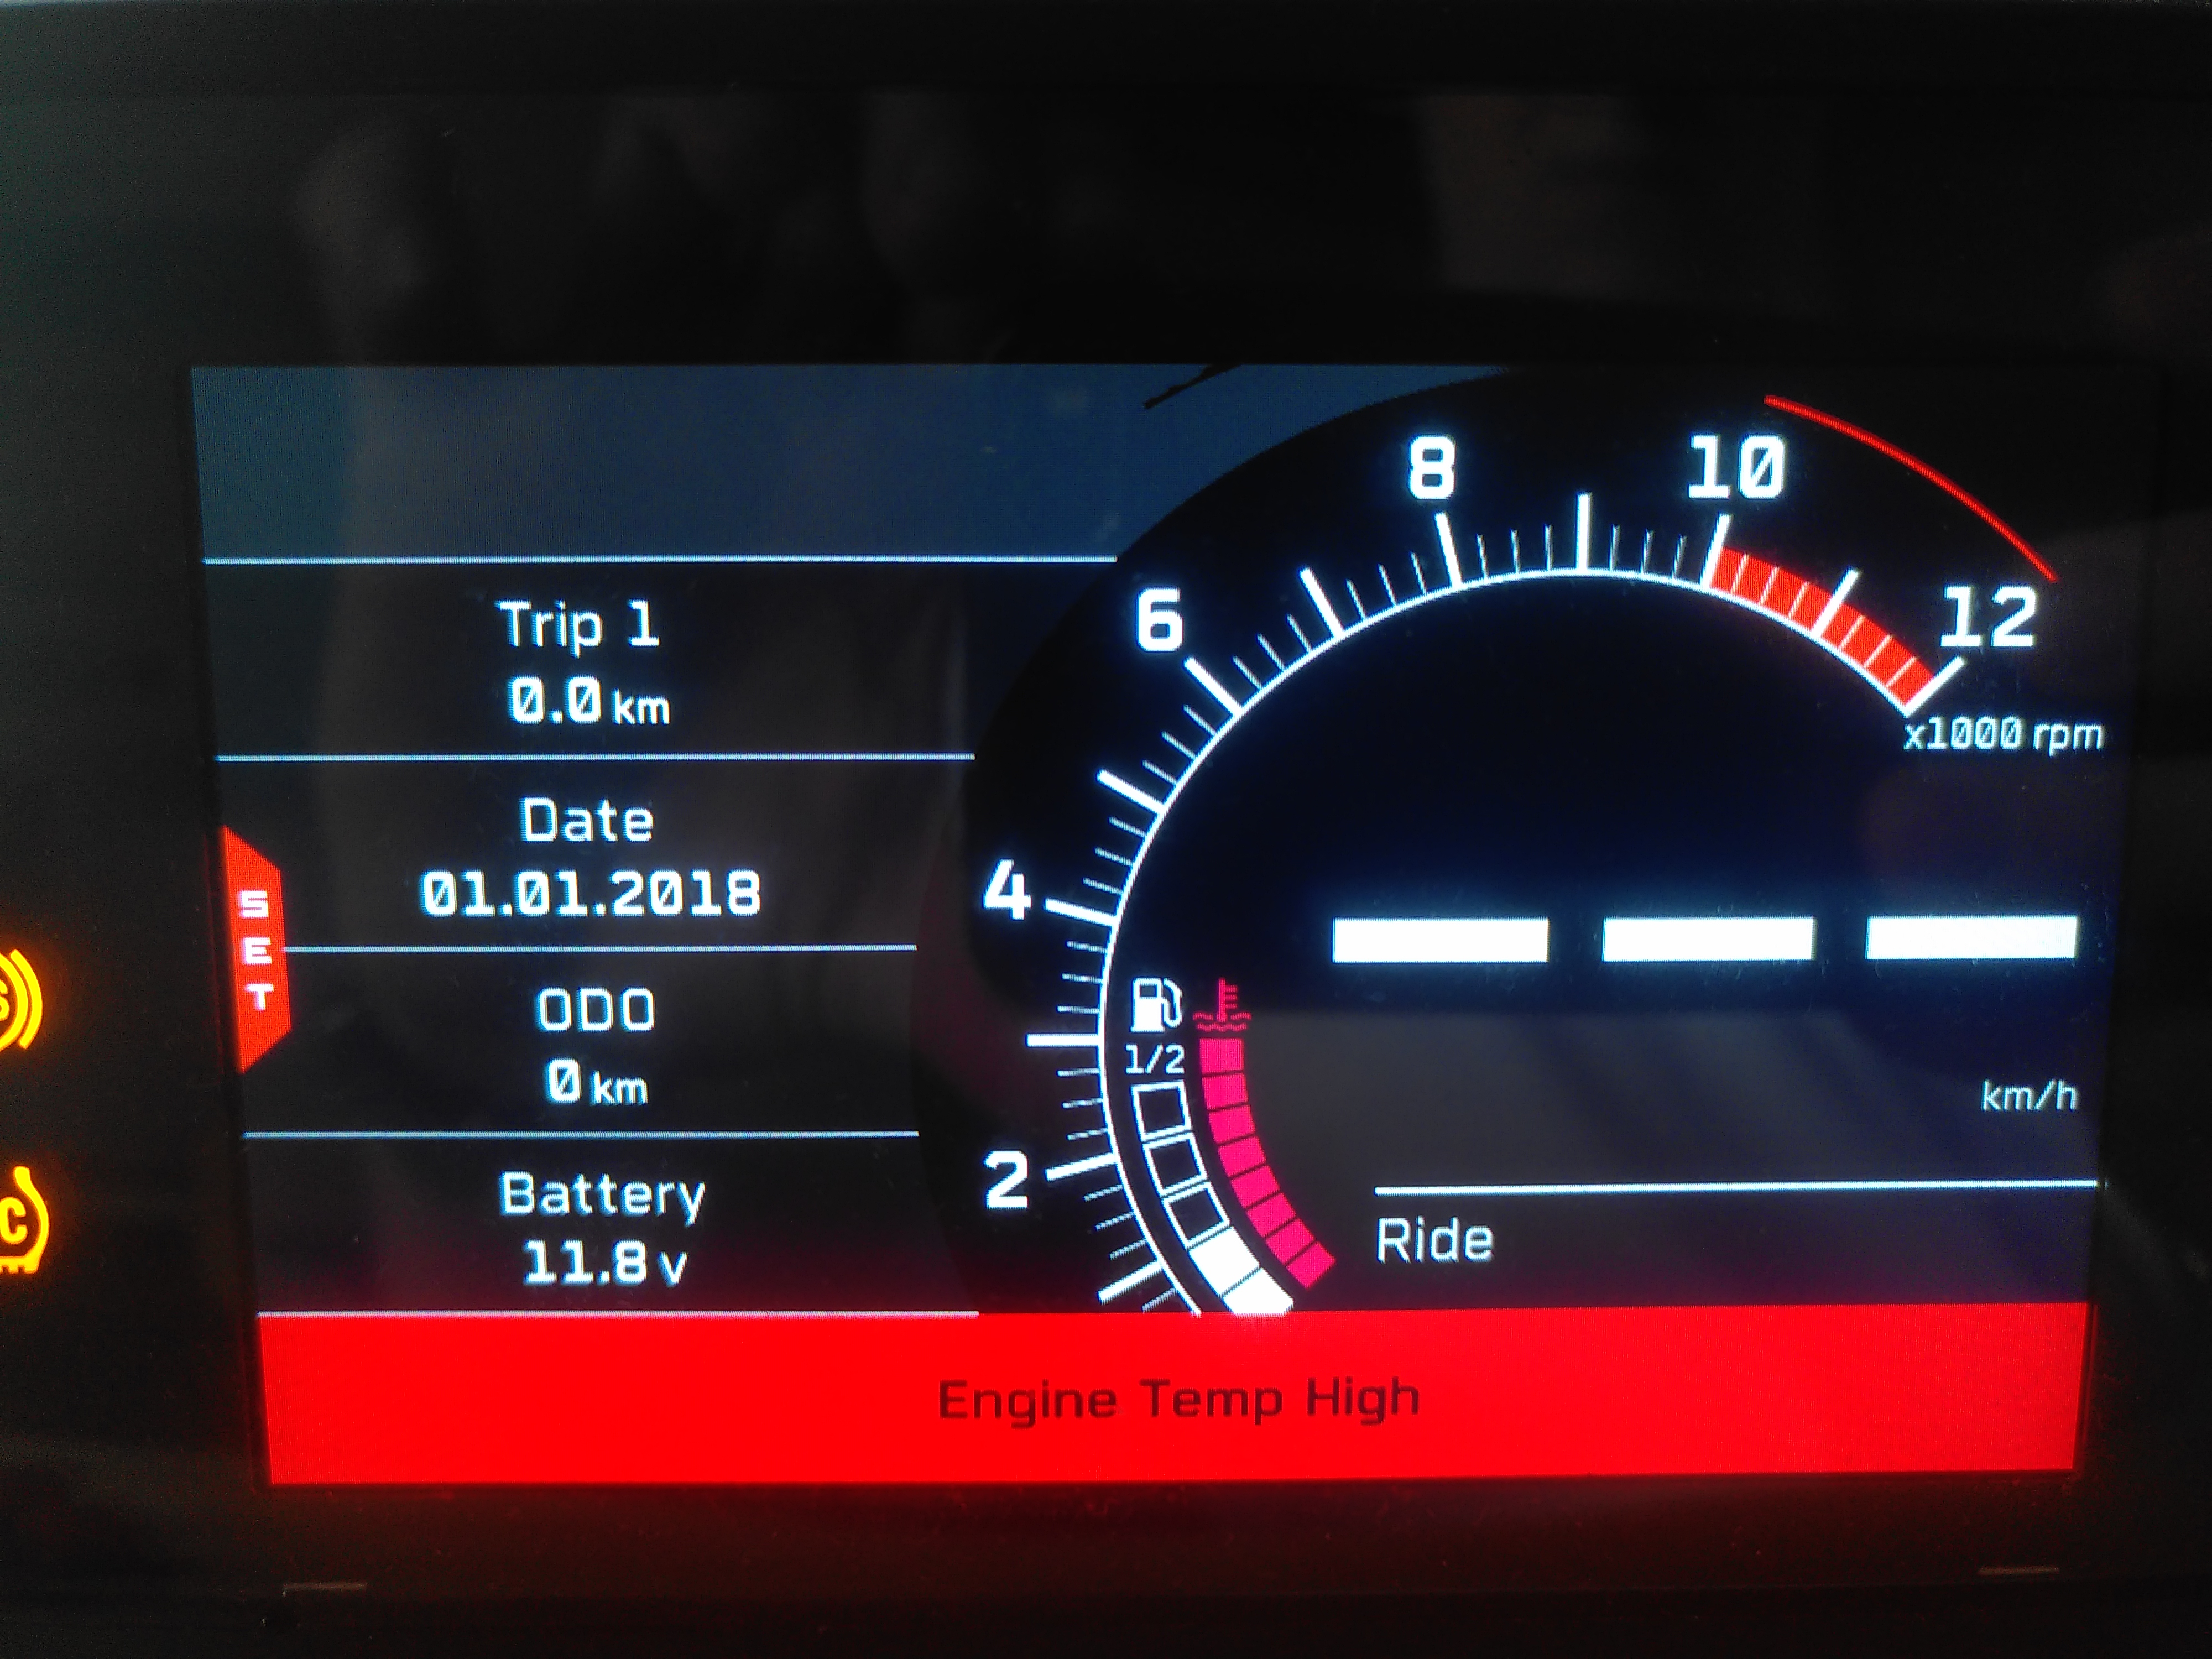
\includegraphics[width=.8\linewidth]{img/demonstration1/result4.jpg}
		\caption{1b}
		\label{fig:sfig2}
	\end{subfigure}
	\caption{The various errors and sensor warnings produced by the Fuzzing Attack.}
	\label{fig:fig}
\end{figure}

According to the CAN messages in the console output most communication occurs on the CAN IDs 0x450, 0x541, 0x551 and 0x552. That is also the range in which the dashboard was able to be influenced the most. This is consistent with online reports by other people trying to reverse engineer the CAN bus on these devices. In order to conclusively decide which CAN ID is responsible for which component, the script might have to be adjusted to run a lot slower and be stopped manually everytime some type of manipulation occurs. That way a specific CAN ID can correlated to a specific part and the packet that was sent can be analyzed further until the structure is correctly identified.

\section{Bluetooth Exploits}
\subsection{Prerequisites}
The amount of connectivity options a car provides is becoming increasingly important to consumers as technology progresses. Many buyers require their car to be able to seamlessly pair to their mobile phone and synchronize contacts, stream media, make phone calls and much more. The industry standard for these features is Bluetooth, since nearly all modern smartphones are equipped with it. Since Bluetooth is often so tightly integrated into the infotainment console on a vehicle and transmits such crucial data, it can prove to be an excellent attack vector for hackers.

Developing the software for an entire onboard entertainment system from scratch can prove to be quite costly for manufacturers. For this reason, most car brands rely on free and open source software as a starting point. The Linux Foundation has created its own project ``Automotive Grade Linux'' (or AGL), complete with a unified code base, to offer companies a platform from which to develop smart features for their vehicles. A lot of the packages in the unified codebase, which is now used by major players in the automotive industry, are simply common Linux packages, which are found in most distributions anyway. And the Bluetooth integration is no exception.\cite{linuxcar}

In order to implement Bluetooth communication the onboard entertainment / navigation system needs to run some sort of protocol stack, which is capable of handling the exchange of information via the Bluetooth standard. One of the most popular implementations of such a stack is `BlueZ'\cite{bluez}, which is the official Linux Bluetooth protocol stack and as such is used on many Linux-based infotainment devices. It is also contained in the aforementioned unified code base provided by AGL. 

%This protocol stack has a substantial market share and is implemented in a large number of products. As is typical with this type of popularity, it is therefore often a target for hackers. In order to secure devices with this implementation, additional security measures can and should be taken. These considerations include, but are not limited to the following:

%\begin{itemize}
%    \item Is the system set up handle secure handshaking?
%    \item Is the system able to ensure proper encryption?
%    \item Is the system detectable via bluetooth at all times?
%\end{itemize}

%A list of vulnerabilities of the bluez daemon can be found here:
%cite https://www.cvedetails.com/vulnerability-list/vendor_id-8316/Bluez.html

For the security conscious, this means that a vehicle behaves just like any other Bluetooth device, since its implementation from a software standpoint does not differ in any meaningful way from any other Bluetooth device. In this demonstration, several traditional Bluetooth exploits will be investigated, which could theoretically target any Bluetooth device.

\subsection{The Bluetooth Standard}
Bluetooth Wireless Technology is a short-range communications system developed by the Bluetooth Special Interest Group since 1998. Numerous versions of the specification exist, with new ones releasing every few years. It is commonly found in mobile devices such as smartphones and headphones, but can also be implemented in Computers, Gaming Consoles, TVs or vehicles.
It boasts a range of up to 400m with the latest iteration, but is typically used  in distances less than 10m. The frequency bands in which Bluetooth is transmitted ranges from 2.4 to 2.4835 GHz. In order to reduce interference with other specifications using this frequency range, this band is divided into 79 different channels, which are 1MHz wide. In case of Bluetooth Low Energy, the band is split into 40 channels with a width of 2MHz each. The very top and bottom of the frequency band is occupied by guard bands, which are 2MHz and 3.5MHz in width respectively.\cite{btspec}
%explain Frequency Hopping
This frequency band is shared by other wireless transmission technologies such as Wi-Fi and LR-WPAN. This unfortunately leads to interference concerns due to the likelihood of packet collisions. If a Bluetooth packet is sent on the same frequency and at the same time as data from another standard, it might simply be lost. To circumvent this, Bluetooth employs Adaptive Frequency Hopping. Here, the two devices switch the channel they use to communicate on each connection event (multiple times a second) in order to minimize the probability of collisions occuring. The sequence the channel sequence the device use is adaptive and channels that are noisy and frequently busy tend to be avoided.
\cite{adaptivefreq}
%explain different Bluetooth Standards
There are two different Bluetooth Standards. The first and oldest one is called Bluetooth Classic, which describes the Bluetooth Basic Rate and Enhanced Data Rate (BR/EDR) standards. In 2006, Nokia developed another specification, which was later integrated into the Bluetooth standard under the name Bluetooth Low Energy. The main differences between the two are their data rates, power consumption requirements, complexity and cost implement and synchronization. A device may also implement both standards at the same time. Security is another important consideration when choosing either of these systems, as we will see in this demonstration.
\cite{btspec}
Whether or not a Bluetooth device advertises its status and is visible to others is determined by the ``Discoverability Mode'' it is set to. The specification for Bluetooth Classic defines three such modes:
\begin{itemize}
	\item Non-discoverable mode, where the device does not respond to an inquiry at all
	\item Limited Discoverable mode, where the device is discoverable only for a limited period of time, during temporary conditions, or
for a specific event.
	\item General Discoverable mode, where the device is discoverable continuously or for no specific condition.
\end{itemize}

Interestingly, many non-discoverable BTLE devices still advertise their status, but broadcast to other devices that their packages should simply be dropped. The downside to this is, that they are still very much visible to attackers, if they choose not to drop these packets.\cite{defcon}

When two devices are paired via classic Bluetooth, they form a so called ``piconet''. In such a piconet, one device is usually designated as the ``master'', while the other acts as a ``slave'' respectively. When pairing wireless headphones to a laptop for example, the former would be the designated slave of said piconet in most cases.

\subsubsection{Bluetooth Adresses}
Every Bluetooth-capable device is identified by a 48-Bit ID, which is assigned to it by the manufacturer. This ID is usually written out as six individual hexadecimal bytes, which are seperated by a colon. For example, a random Bluetooth Adress might look like this:
\begin{verbatim}
DE:AD:12:34:CA:FE
\end{verbatim}


This adress can be broken up into several parts filling a different purpose. The lower 24 Bits of this adress (starting from the MSB) are also called the ``Organizationally Unique Identifier (OUI)''. This OUI is further divided into the ``Non-significant Address Part (NAP)'' and the ``Upper Address Part (UAP)'', each being 2 Bytes and 1 Bytes respectively. The purpose of the UAP is being the seed for various Bluetooth specification algorithms, while the NAP is used in Frequency Hopping Schemes. When trying to identify a Bluetooth device or piconet, the NAP can be neglected. The UAP is of definite importance, but this will be demonstrated later.\cite{btspec}
\begin{figure}[!h]
    \begin{center}
        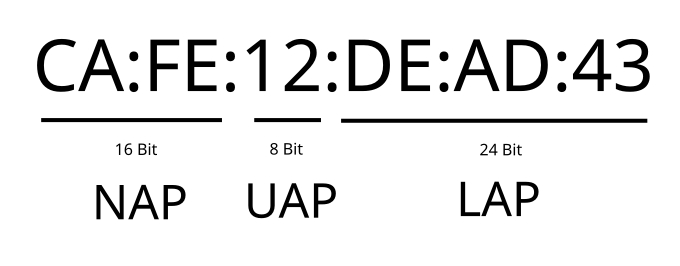
\includegraphics[width=.8\linewidth]{img/demonstration2/BT_ADDR.jpg}
        \caption{The components to a Bluetooth Address}
    \end{center}
\end{figure}


\subsection{Setting up the Ubertooth One}
In order to demonstrate how easily Bluetooth devices can be tracked, identified and their packets possibly intercepted and sniffed, this demonstration will use the capabilities of the Ubertooth One. Its features were already discussed in section \ref{ubertoothintroduction}. In order to use the Ubertooth it simply needs to be connected to one of the USB ports of any PC and its host code as well as the Bluetooth Baseband Library installed. The latter can be done by running the following commands on a Linux machine.

\begin{verbatim}
    wget https://github.com/greatscottgadgets/libbtbb/archive/\ 
        2020-12-R1.tar.gz -O libbtbb-2020-12-R1.tar.gz
    tar -xf libbtbb-2020-12-R1.tar.gz
    cd libbtbb-2020-12-R1
    mkdir build
    cd build
    cmake ..
    make
    sudo make install
    sudo ldconfig
\end{verbatim}

In order to install the Ubertooth host code, it first has to be cloned from its repository. Once this is done a build directory can be created and the tools can be built and installed using cmake.
\begin{verbatim}
    wget https://github.com/greatscottgadgets/ubertooth/releases/download/\
        2020-12-R1/ubertooth-2020-12-R1.tar.xz
    tar -xf ubertooth-2020-12-R1.tar.xz
    cd ubertooth-2020-12-R1/host
    mkdir build
    cd build
    cmake ..
    make
    sudo make install
    sudo ldconfig
\end{verbatim}

Once the required software is installed on the host machine and the Ubertooth One is connected, a good way to test the functionality is to run ``ubertooth-specan-ui'', a binary, which is found as part of the Ubertooth host code.
Its purpose is to create a graph plotting the activity over the entire 2.4GHz radio band frequency spectrum, which is updated in real time.
Figure \ref{fig:blfreqspec} shows the generated graph. Each of the green spikes represents a different channel upon which data is being sent. If a beacon is found during the scan, it is represented by a white spike. The red line continuously hops around to signify the center of any given frequency channel.

\begin{figure}[!h]
    \begin{center}
        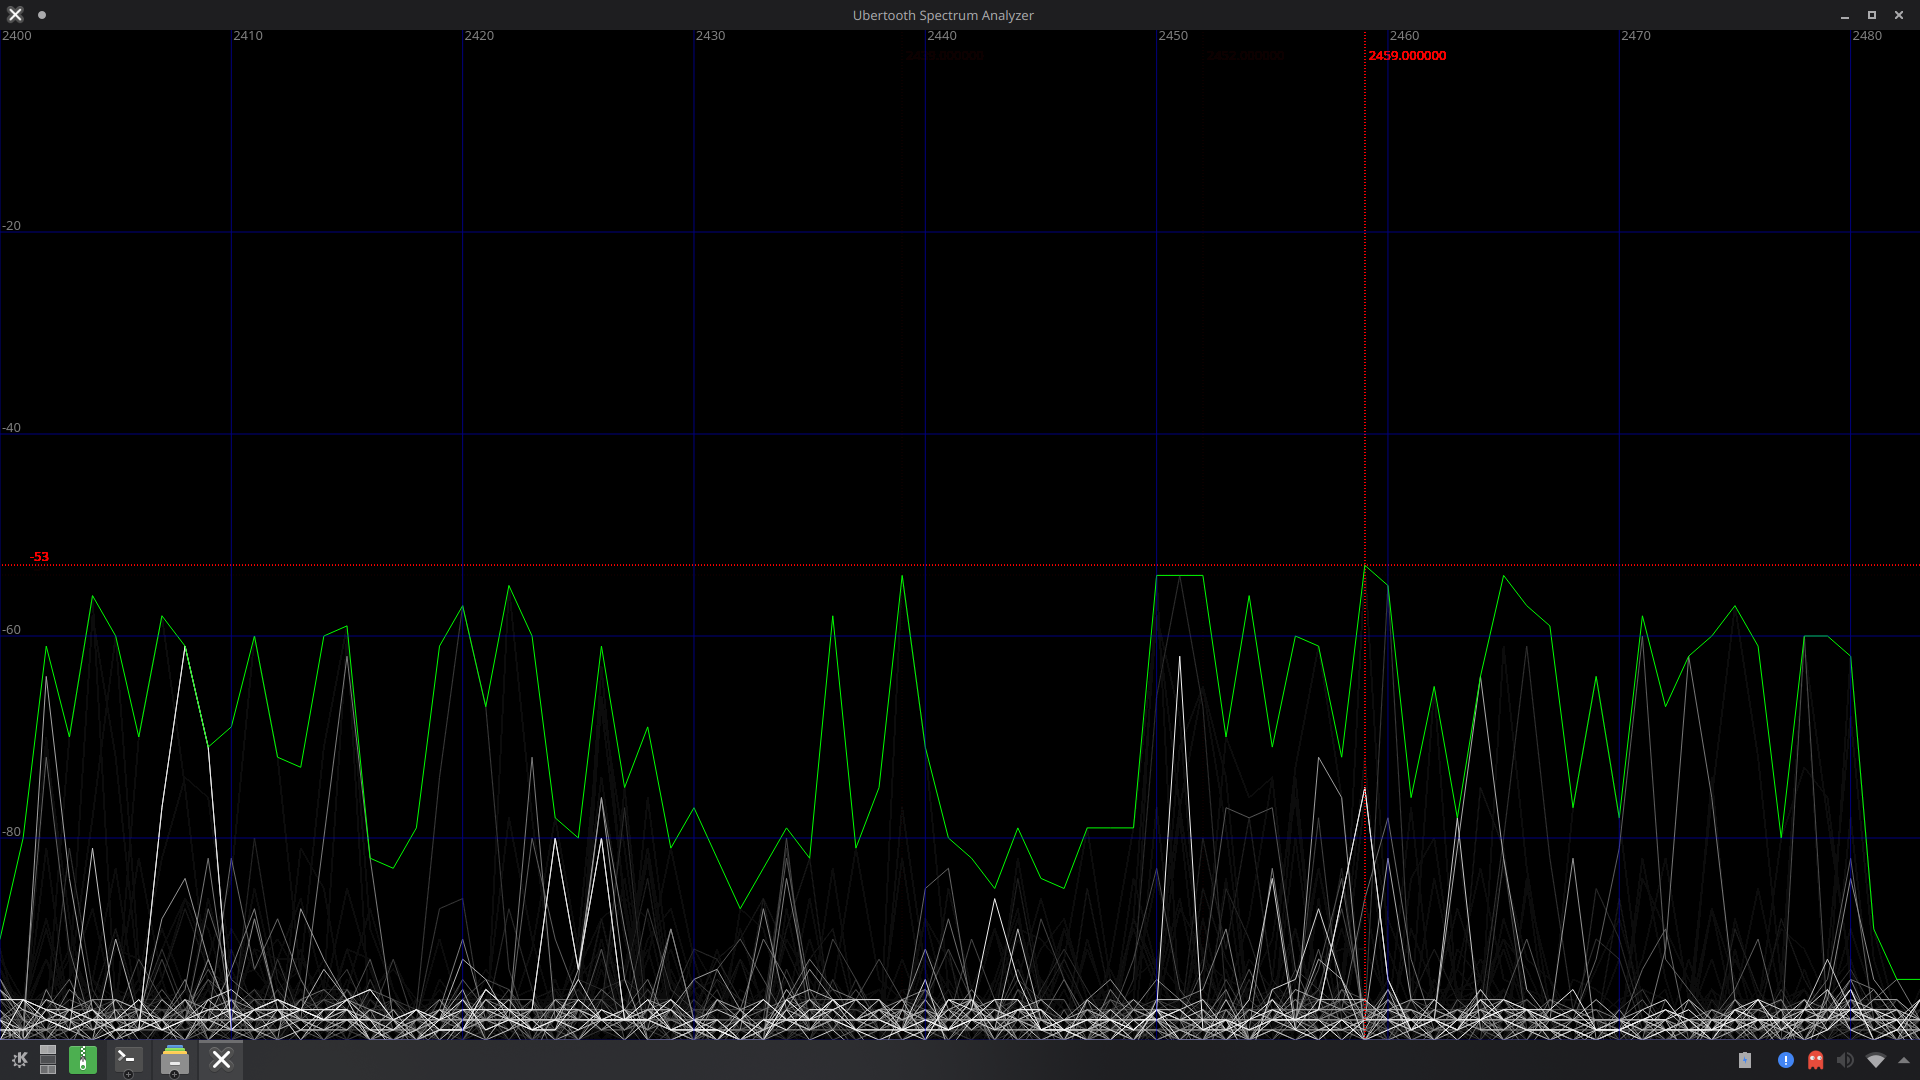
\includegraphics[width=.8\linewidth]{img/proof-of-concept/ubertooth-specan.png}
        \caption{Signals along the Bluetooth frequency spectrum}
        \label{fig:blfreqspec}
    \end{center}
\end{figure}

\subsection{Detecting Bluetooth Devices using ubertooth-rx}
\label{ubertooth-detection}

One of the easiest ways to use the Ubertooth for reconnaissance is to simply check for available Bluetooth devices in the area as a first step. For this purpose, the command ``ubertooth-rx'' can be used in combination with the flags ``-z'' for survey mode and ``-t'' to specify a search time duration. This can be used to find all Bluetooth devices in the area that are transmitting a Bluetooth (Classic) signal.\cite{ubertoothrx}

The output of this command is a list of all the Bluetooth Adresses, which were found. The biggest downside with discovering devices in this way is that no information other than the LAP and on some devices the UAP is being shown. For this purpose, exploits like BlueHydra can be used, which will be demonstrated shortly.
\begin{verbatim}
sudo ubertooth-rx -z -t 60
\end{verbatim}
\begin{verbatim}
    Survey Results
    ??:??:10:17:30:28
    ??:??:??:65:62:6D
    ??:??:85:5E:0E:94
    ??:??:??:4A:A8:87
    ??:??:??:09:0D:F7
    ??:??:??:AB:BB:8E
\end{verbatim}

A Bluetooth Piconet is identified by the LAP and UAP of the master device. The first and third line in the example output show such a case. As mentioned before, the first two Bytes of the Bluetooth Adress make up the Non-Significant Address part and therefore do not have to be known in order to merely contact the device. This means just with the information provided by this simple scan, an attacker could try to connect to these piconets and return the device names and possibly more information in the process. This attack also works for devices which are set to be ``undiscoverable''. The name of the devices might be found by simply running hcitool:\cite{https://github.com/greatscottgadgets/ubertooth/blob/master/host/doc/ubertooth-rx.md}

\begin{verbatim}
hcitool name 00:00:BF:8E:39:B6
Fairphone 3
\end{verbatim}

An even better way to identify Bluetooth Devices in the area would be by using an exploit like BlueHydra, which will be demonstrated next.

\subsection{Detecting Bluetooth Devices using BlueHydra}
`BlueHydra'  is a tool built on the BlueZ library which can be used to fingerprint Bluetooth devices in the vicinity, regardless if they are communicating via Bluetooth Classic, Low Energy or what their discoverability settings are (as long as they advertise themselves in some way).\cite{bluehydragit} In addition to finding them, BlueHydra also provides useful information about the properties of a device like its name, manufacturer or even the distance from the attacker in the case a protocol like iBeacon is used.

Blue Hydra was initially presented at DEFCON in 2016. Since the code originally written to demonstrate this exploit relies on Python2 and older versions of the BlueZ stack, the easiest way to run it is to utilize some kind of Debian derived Linux distribution in order to easily install these dependencies. BunsenLabs Beryllium was chosen for this demonstration.

As opposed to Wi-Fi, Bluetooth does not posess any kind of ``monitor'' mode as per the specification. Comparable Bluetooth discovery tools like ``Redfang'' circumvent this by brute forcing the six bytes of the bluetooth address. This means the program simply iterates over every possible combination of these bytes and queryies the devices corresponding to these addresses for their name, until an answer is received.\cite{redfang}

In order to discover Bluetooth devices in the area without brute forcing, BlueHydra instead relies on concepts taken from the the BlueZ test scripts as well as Linux packages like ``hcitool'' and ``hciconfig''. These concepts are used in parallel with the Ubertooth hardware (otpionally, if it is present on the system).\cite{defcon}


In order to handle the actual Bluetooth communication, BlueHydra mostly relies on ``btmon'', which is a tool included in the Bluez library. btmon monitors all commands that the operating system is sending and receiving from one or more connected Bluetooth Adapters and organizes these commands into one long text stream. 
Essentially there are multiple threads constantly executing and parsing the data supplied by btmon. The parsed data is then analyzed and grouped per device so that BlueHydra always knows when there are new devices communicating with the system.

Parallel to the execution and parsing of btmon, another thread is used to constantly discover new devices. This discovery thread uses the BlueZ test scripts to search for Bluetooth classic devices, listens for BTLE advertisements, uses ``hcitool'' to retrieve more information on a device and also periodically tests if a device is still present by using ``i2ping''.

One of the key differences between BlueHydra and the regular bluetooth implementation found in the Linux Kernel is that as mentioned previously, the Kernel discards advertisement packages from BTLE devices, which are set to be non-discoverable. BlueHydra instead very much processes these packages and uses them to fingerprint these hidden devices.

When an Ubertooth is present in the system, a seperate thread also runs ubertooth-rx, just like it was demonstrated in the previous section. Additionally, a thread for the command-line user interfacing and data processing exist, but these threads are not relevant to this demonstration so they will not be elaborated further.


Once a distribution with the apt-package manager was installed, the necessary dependencies were obtained using the following commands:

\begin{verbatim}
    sudo apt-get install bluez bluez-test-scripts python3-bluez \
        python3-dbus libsqlite3-dev ubertooth
    sudo apt-get install ruby-dev bundler
\end{verbatim}

Since the Blue Hydra Script is written in Ruby, version 2.1 of the language or higher has to be installed in addition to these packages. The BlueZ version provided needs to be at least Version 5.

After this step was complete, the Blue Hydra source code was downloaded from the official Git repository. It is important to note that the current release is no longer maintained by the original creators pwnieexpress, but rather one of the people involved by the name of ``ZeroChaos-''.

In order to execute the provided Ruby script, the downloaded files can be extracted anywhere in the file system. A shell has to be opened at the location of the extracted files and the following commands can be run in order to download the required Ruby Gems and run the actual script:

\begin{verbatim}
    bundle install
    ./bin/blue_hydra
\end{verbatim}

It is important to note that the blue\_hydra command needs to be run with root-privileges in order to work. The script will now use the Ubertooth hardware as well as the Bluetooth adapter in order to track nearby bluetooth devices in real time. An example of the command line output is shown in figure \ref{fig:bluehydraoutput}.

\begin{figure}[!h]
    \begin{center}
        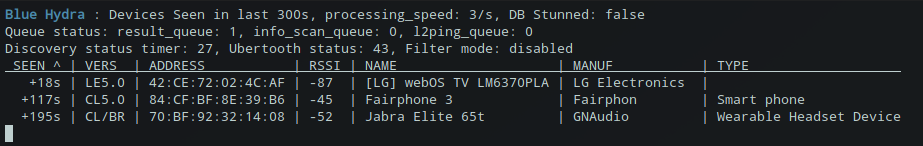
\includegraphics[width=.8\linewidth]{img/demonstration2/blue_hydra_output.png}
        \caption{The output of Blue Hydra}
        \label{fig:bluehydraoutput}
    \end{center}
\end{figure}

In this case, a Smart TV, a Smartphone and a pair of headphones was detected.

The real-time results are organized in a table. The table can be sorted by any of its columns by using the ``S'' or ``s'' keys, with ``r'' being used to reverse the sort order. The ``c'' key can be used to change the column set alltogether. Additionally, the table can be filtered by using the ``F'' or ``f'' key. Execution can be interrupted by typing ``q''.

The information displayed includes the last time the device was picked up by the system in seconds, the Bluetooth protocol used for communication, the device address, its name, manufacturer any more. From this point the Bluetooth adress can be used in order to specifically target a certain device or piconet.

%\subsection{Gathering information using ubertooth-scan}

%In order to find even more information about devices the command ``ubertooth-scan'' can be used in combination with the Ubertooth hardware. This command performs an inquiry scan as well as an extended inquiry scan using a regular Bluetooth adapter. Simultaniously it searches for nearby devices using the Ubertooth as demonstrated before.

%The goal of this is to find out about the features supported by some device using this command. For this reason the flags ``-s'' is used in order for the utility to use BlueZ to scan for discoverable devices and the ``-x'' flag in order to retrieve the device feature page. The output of this command might look as follows:

%\begin{figure}[!h]
%    \begin{center}
%        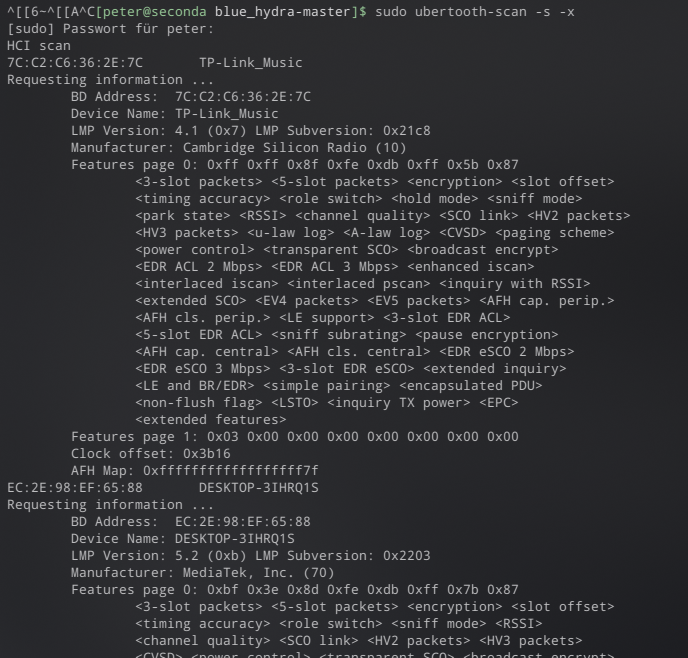
\includegraphics[width=.8\linewidth]{img/proof-of-concept/ubertooth-scan.png}
%        \caption{example output of ubertooth-scan -s -x}
%    \end{center}
%\end{figure}

\subsection{Sniffing Bluetooth Packets with ubertooth-btle}

Once a suitable victim device was identified, packages sent over the Bluetooth connection can be sniffed by using either ``ubertooth-btle'' or ``ubertooth-rx'', depending on whether the target is using Bluetooth Classic or the Bluetooth Low Energy Standard. For the remainder of this demonstration we will focus on BTLE communications.

In order to use Bluetooth Low Energy devices, they must be paired first. Pairing is the process by which two devices establish a connection for the first time and trade secrets so that a secure, encrypted connection can be established. When a connection between two paired devices is terminated, the secrets established during the pairing process get saved on both devices, so the next time they connect, they do not need to be paired again.

Data transferred via Bluetooth Low Energy is usually AES-CCM encrypted. This should make a man-in-the-middle attack improbable, since AES encryption is considered very secure. Unfortunately the key exchange protocol used in this standard does not hold up to this level of security and can be exploited.

The key exchange between two BTLE devices happens in two phases. During Phase 1, the initiating device sends a pairing request, upon which both participants exchange their respective capabilities including authentication requirements, maximum key size, available I/O and such. This data is sent unencrypted. During Phase 2 the devices generate or exchange the temporary key that will be used based on the pairing mode. These modes and the significance of the temporary key will be explained next.

The Bluetooth Low Energy Standard describes three different methods of pairing, which differ slightly between the different versions of the standard (4.0, 4.1 and 4.2). Devices using the 4.0 and 4.1 standard use the so called ``LE Legacy Pairing'' process, while newer devices are able to use the safer ``LE Secure Connections'' process. These devices are also backwards-compatible to LE Legacy Pairing however, and are therefore not safe by default.

The LE Legacy Pairing modes are the following:
\begin{itemize}
    \item JustWorks (TM)
    \item Passkey
    \item Out Of Band (OOB) Pairing
\end{itemize}

The commonality between all these modes and the reason the pairing process is considered unsafe is that each of them rely on a so called ``Temporary Key''. This key is used to generate a ``Short Term Key'', with which the connection is then encrypted. The temporary key (TK) is exchanged between the devices when they first pair and differs in its attributes depending on the pairing process, that is being used.

For JustWorks, the TK always has a value of zero as per the standard and therefore does not even need to be brute forced at all. In Passkey Mode, the TK is a decimal value six digits in length, meaning it can have any value between 0-999.999. An attacker could feasibly brute force this value in around a second, as shown in the demonstration of crackle, a tool designed specifically for this task. The usefulness of Crackle will be described in the next demonstration. Only OOB Mode is theoretically capable of protecting the temporary key from Brute Force Attacks, because the key can be up to 128 Bit in size in this mode. Unfortunately OOB pairing is fairly complex compared to other modes and therefore rarely implemented in practice.

If an eavesdropper listens to the initial pairing process of two devices using Bluetooth Low Energy, it would be very easy for them to acquire this temporary key (assuming JustWorks or Passkey mode was used), which would allow them to listen for the exchange of the short term key and thereby allow them to decode all future communication occuring within this piconet. 

Even if the attacker missed the original pairing process, an attack using crackle is still feasible by just jamming the connection, thereby forcing the two devices to reconnect and exchange keys once more.

Thankfully, the Ubertooth Host code provides a utility for both eavesdropping on a Bluetooth Low Energy connection as well as purposefully disconnecting said connection. The command ``ubertooth-btle''  can be used in combination with the flags ``-i'' for dropping the existing connection, ``-f'' in order to follow a specific device via its Bluetooth address and ``-q'' in order to save the eavesdropped packages to a Packet Capture (PCAP) file.\cite{ble4sec}

\begin{verbatim}
ubertooth-btle -i -f 39:30:82:4E:87:2F -q test20230703.pcap
\end{verbatim}

The recorded .pcap file can be opened with an application like Wireshark, which was described in section \ref{wiresharkintro}. Here, the packets sent by each device in the piconet can be analyzed. For example, the ``ADV\underline{}IND'' packets  signal that a peripheral device was just powered on and is looking to connect to any node.

\begin{figure}[!h]
    \begin{center}
        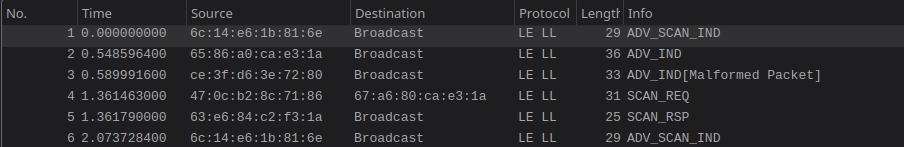
\includegraphics[width=.8\linewidth]{img/demonstration2/ble_communication_pcap.png}
        \caption{packets captured by Ubertooth during BLE communication}
    \end{center}
\end{figure}

Devices using LE Secure Connections, so starting with BTLE 4.2, instead rely on a single long term key. This key is generated using Elliptic Curve Diffie Hellman cryptography and is therefore regarded as significantly more secure. These devices are also backwards-compatible to LE Legacy Pairing however, and are therefore not safe by default.

\subsection{Decoding BTLE communication via crackle}

This security flaw in the key exchange of the BTLE standard was quickly discovered by researchers and led to the development of a tool called ``crackle'', which was first demonstrated at SchmooCon 9. \cite{mikeryancrackle}

Once a connection between two devices has been eavesdropped on and saved to a PCAP file, crackle can be used to automatically find the pairing messages, brute force the temporary key and decode the entire communication. The decoded, readable data is then dumped to another PCAP file.

Crackle can be downloaded from its official repository. A makefile is supplied, so the tool can simply be installed on a Linux machine by navigating to the previously downloaded folder and running the following command:

\begin{verbatim}
sudo make install
\end{verbatim}

Once installed, it can be invoked from anywhere by running ``crackle''. The tool possesses two distinct modes of operation. It is able to either crack the temporary key of a recorded PCAP file or decrypt an entire communication if a suitable Long Term Key is supplied.
The ``Crack TK'' mode is the default operation of the tool and is invoked as soon as a PCAP file is supplied via the ``-i'' option. Once the TK is successfully recovered, crackle will still recover the remaining keys and decrypt all following packets. Once a LTK is found, it will be printed.

If the LTK is already known, it can simply be supplied via the ``-l'' flag. If this flag is passed to crackle, it will simply decrypt the supplied communication. In case an output file is supplied via the ``-o'' flag, the decrypted packets can also be printed to an output file.\cite{mikeryancrackle}

Since a device that uses Bluetooth Legacy Pairing was not available for this demonstration, test scripts that are supplied with the crackle utility are used to demonstrate this functionality instead. These come in the form of PCAP files, just like they would have been captured using the ``ubertooth-btle'' command mentioned above.

\subsubsection{Cracking JustWorks (Temporary Key is always 0000)}
In the first testcase, two devices using JustWorks pairing were eavesdropped. The messages exchanged during the pairing process was saved to a PCAP file and looks as follows when opened in Wireshark:

\begin{figure}[!h]
    \begin{center}
        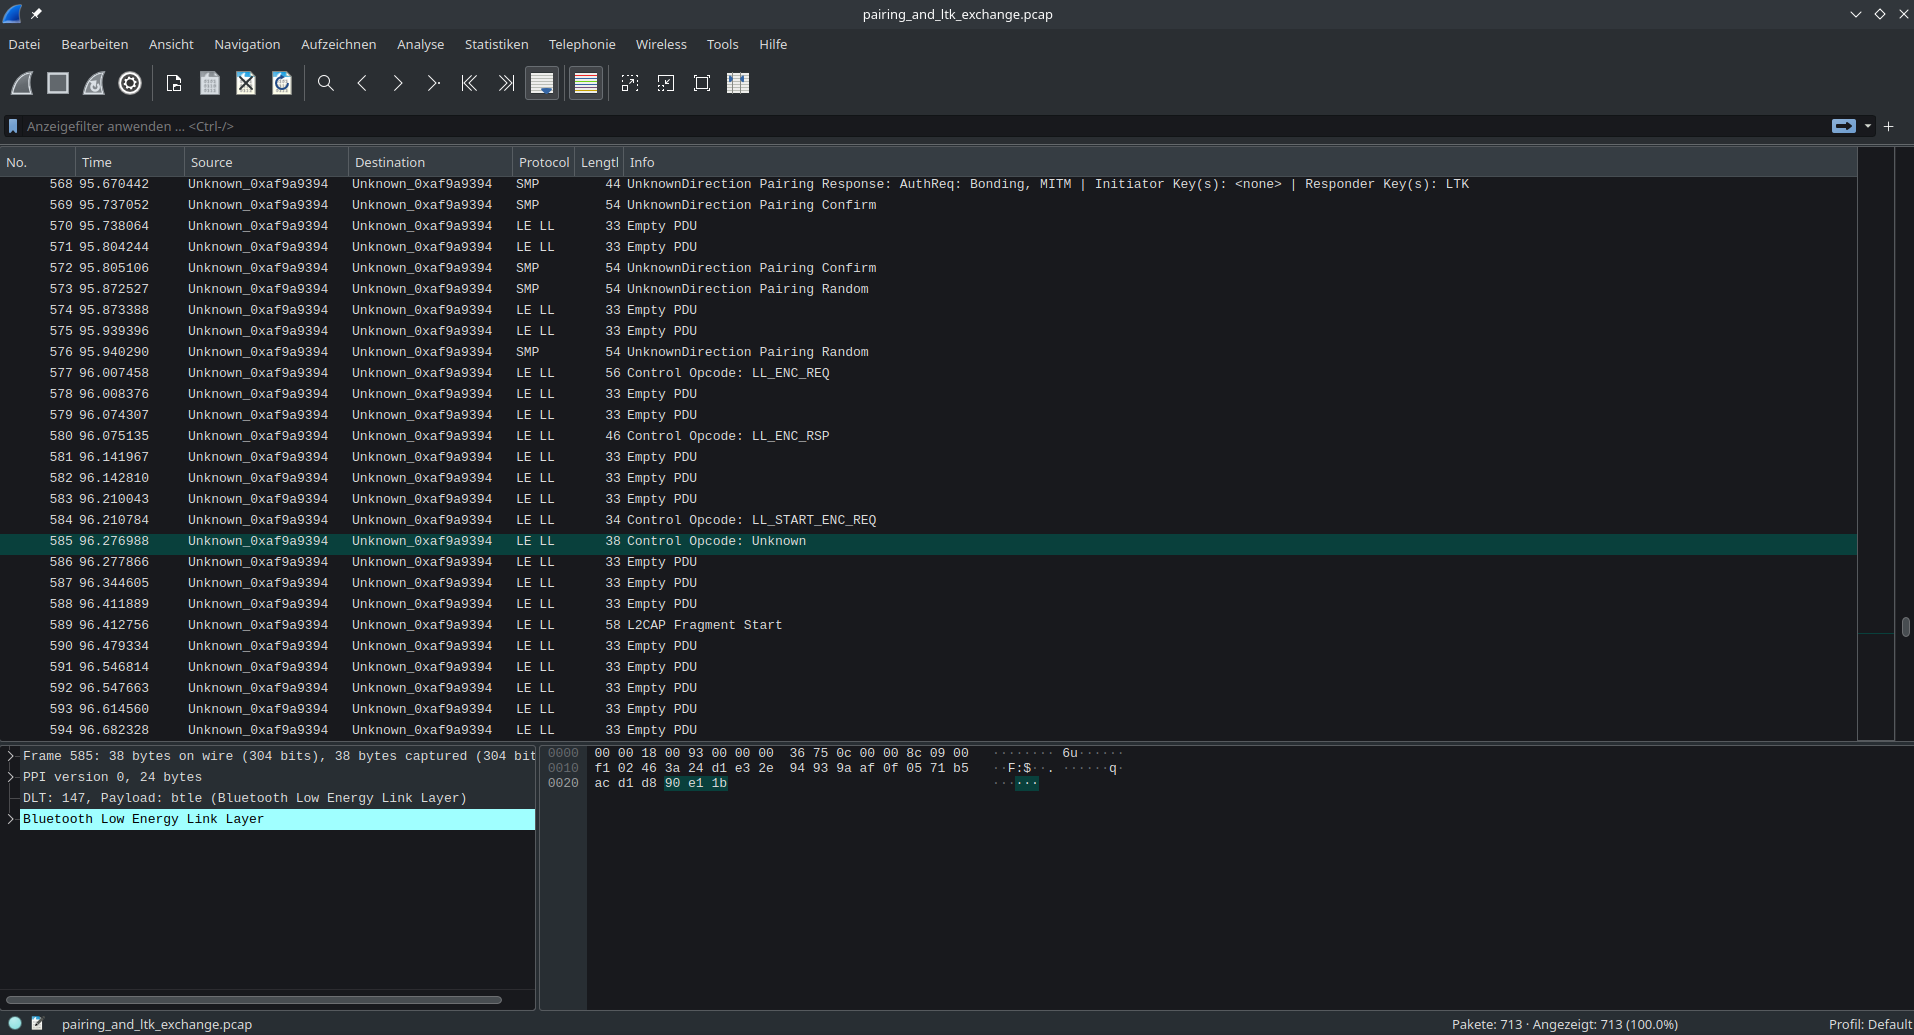
\includegraphics[width=1\linewidth]{img/demonstration2/crackle01_before.png}
        \caption{Bluetooth Low Energy Packets exchanged during a JustWorks pairing process}
    \end{center}
\end{figure}
Note that after the ``LL\_START\_ENC\_REQ'' packet the traffic is encrypted and can no longer be deciphered.

Crackle can now be invoked using the following command. Note that both an input and output file are supplied using their respective command line options:
\begin{verbatim}
/usr/local/bin/crackle -i 01_crack/pairing_and_ltk_exchange.pcap -o 01_crack/out/actual_output.pcap
Found 1 connection

Analyzing connection 0:
  08:3e:8e:e1:0b:3e (public) -> 78:c5:e5:6e:dd:e8 (public)
  Found 3 encrypted packets
  Cracking with strategy 0, 20 bits of entropy

  !!!
  TK found: 000000
  ding ding ding, using a TK of 0! Just Cracks(tm)
  !!!

  Decrypted 3 packets
  LTK found: 7f62c053f104a5bbe68b1d896a2ed49c

Decrypted 3 packets, dumping to PCAP
Done, processed 713 total packets, decrypted 3
\end{verbatim}

As seen in the console output the TK was successfully guessed as being 0000, as is the norm with this pairing process, and even the LTK was recovered. Additionally, the previously encrypted packets in the input file were successfully decrypted and saved to the output file. Again, this can be opened in Wireshark and now looks as follows:

\begin{figure}[!h]
    \begin{center}
        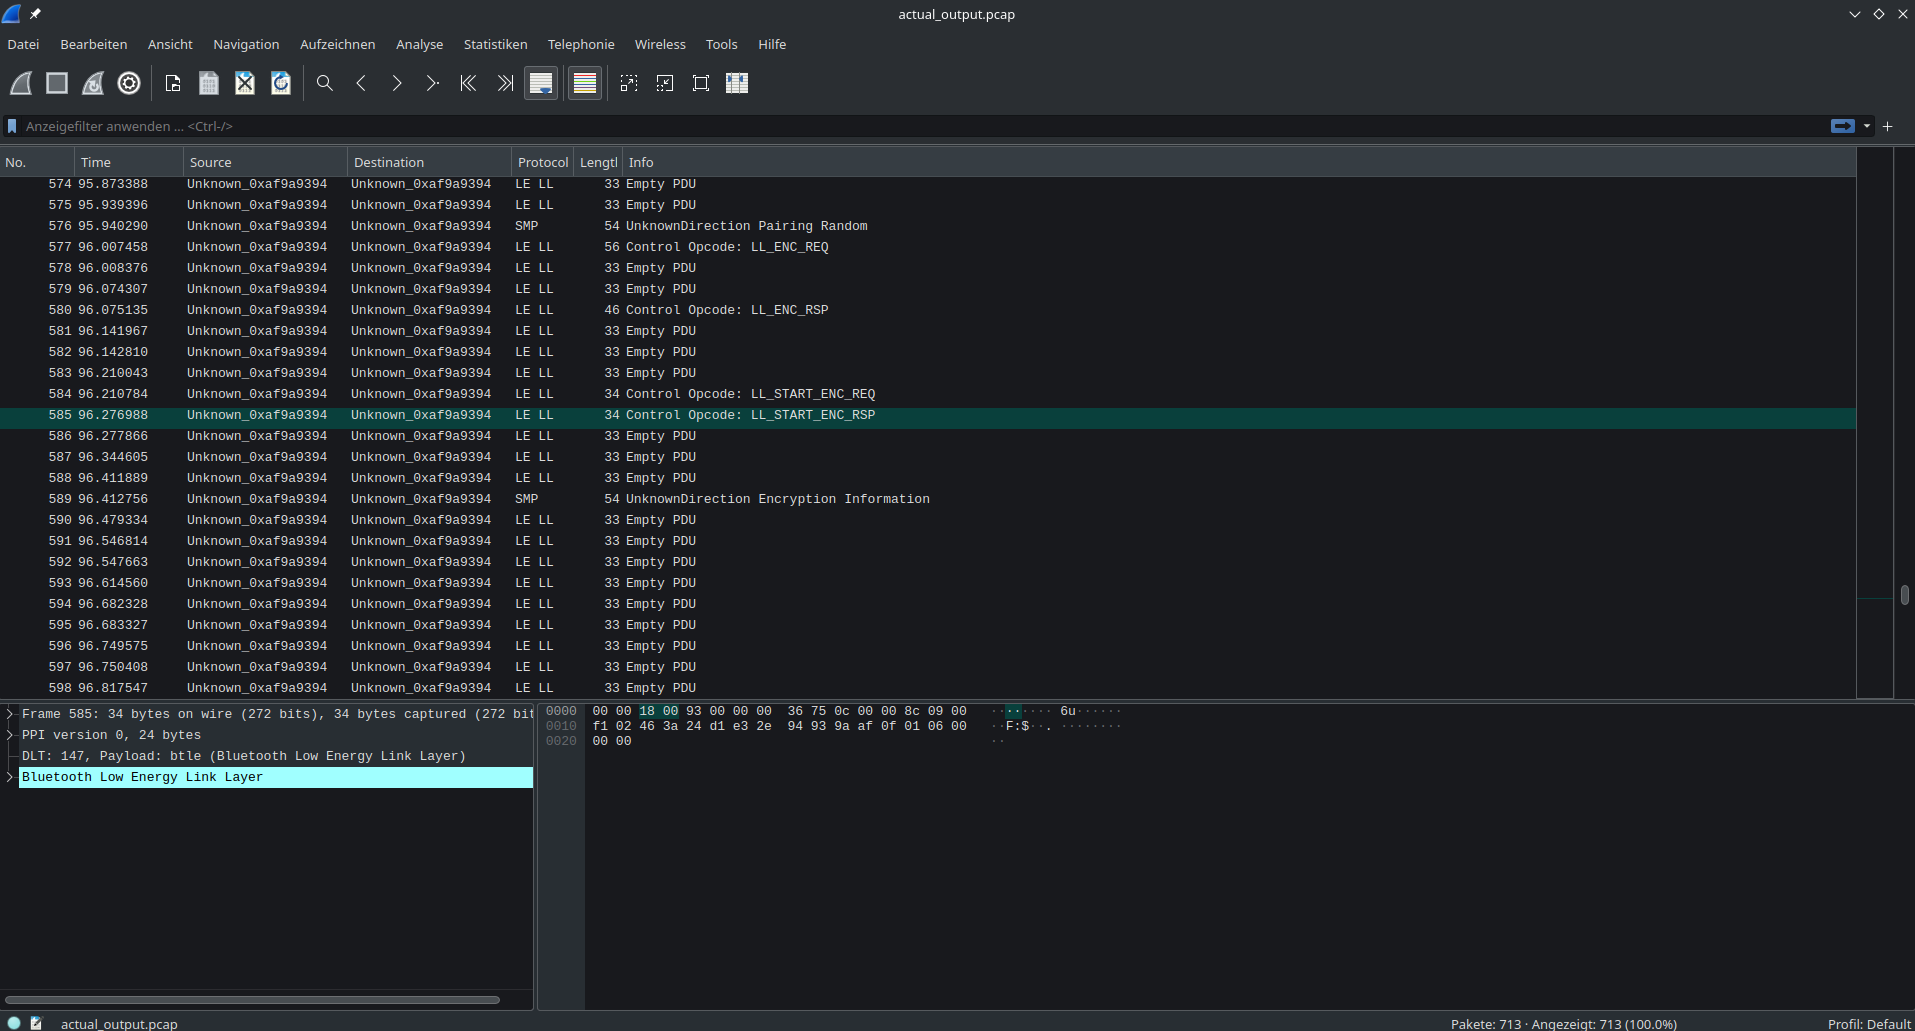
\includegraphics[width=1\linewidth]{img/demonstration2/crackle01_after.png}
        \caption{Bluetooth Low Energy Packets decrypted past the pairing process}
    \end{center}
\end{figure}
Here, the packets below ``LL\_START\_ENC\_REQ'' are decrypted and readable.

\subsubsection{Using the TK to decrypt the LTK}
The previously found LTK can now be used to decrypt any communication between these two devices. In another PCAP file, a communication in this piconet was eavesdropped, but the pairing process was not observed. By passing the LTK via its designated flag, crackle will instead operate in decrypt-only mode. In this mode, the communication will be decrypted and saved to a desired output file, without trying to recover any keys.
\begin{verbatim}
/usr/local/bin/crackle -i 02_ltk_decrypt/known_ltk.pcap -o 02_ltk_decrypt/out/actual_output.pcap  -l 7f62c053f104a5bbe68b1d896a2ed49c
Warning: packet is too short to be encrypted (2), skipping
Found 1 connection

Analyzing connection 0:
  08:3e:8e:e1:0b:3e (public) -> 78:c5:e5:6e:dd:e8 (public)
  Found 10 encrypted packets
  Decrypted 7 packets

Decrypted 7 packets, dumping to PCAP
Done, processed 303 total packets, decrypted 7

\end{verbatim}

As seen in the console output, most (though not all) packets could be decrypted and were saved to the output file. The differences between the two files can again be compared in Wireshark. Highlighted here is the termination of the connection and it is very clearly visible that this previously unknown packet (left) was successfully decrypted (right).\cite{mikeryanyt}
\begin{figure}[!h]
    \begin{center}
        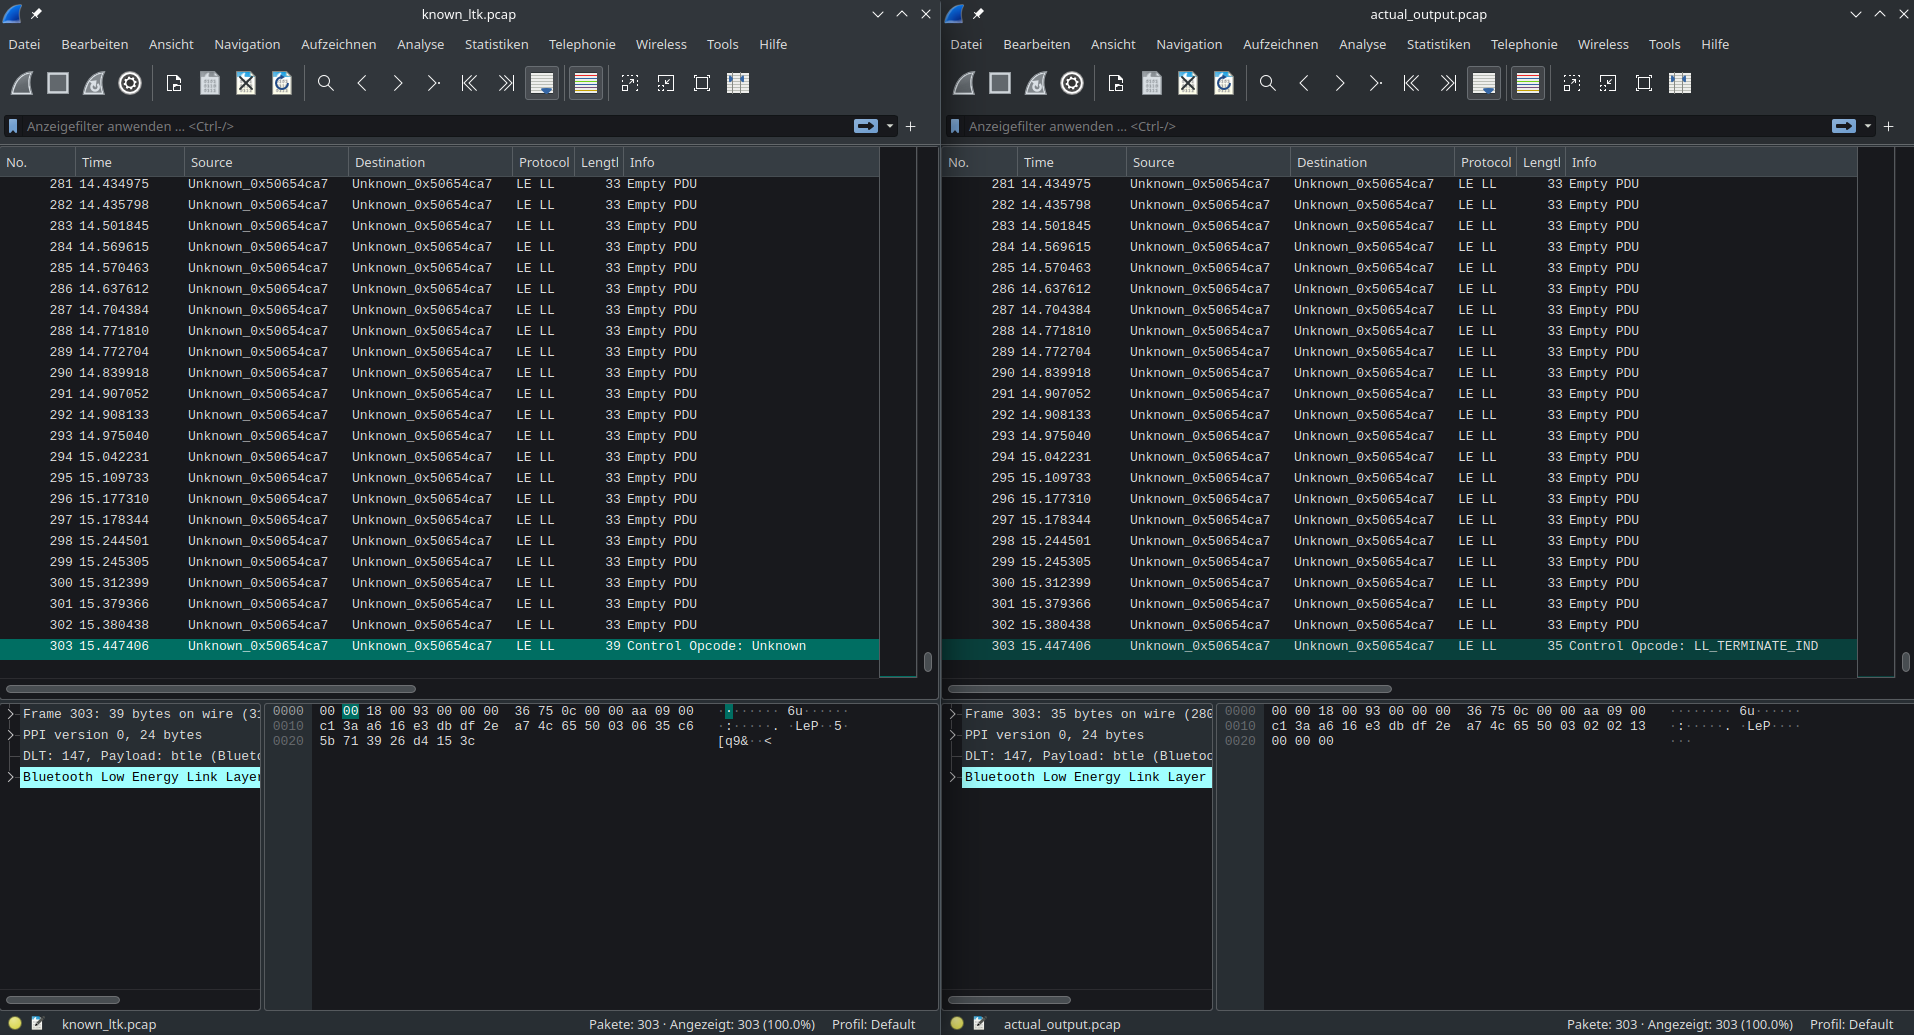
\includegraphics[width=1\linewidth]{img/demonstration2/crackle02_after.png}
        \caption{Bluetooth Low Energy Packets decrypted with the known LTK}
    \end{center}
\end{figure}

%Decrypting communication
%\subsubsection{Cracking Passkey (random six-digit Temporary Key)}
%\begin{verbatim}
%/usr/local/bin/crackle -i 03_stk_brute/missing_confirms.pcap -o 03_stk_brute/out/actual_output.pcap
%/usr/local/bin/crackle -i 04_le_secure_connections/le_secure_connections.pcapng -o 04_le_secure_connections/out/actual_output.pcap
%/usr/local/bin/crackle -i 05_numeric_pin/numeric_pin.pcap -o 05_numeric_pin/out/actual_output.pcap
%\end{verbatim}



As mentioned before the BTLE standard 4.2 abandons the custom key exchange protocol in favor of a Diffie-Hellman key exchange. This is also the reason crackle is unable to decode packets which were transferred via these connections. If crackle detects that LE Secure Pairing was used, it throws an error and immediately exits without trying to crack the pairing.\cite{ble4sec}

\section{Keyfob RFID Attacks}
\subsection{Prerequisites}
When unlocking a vehicle via a remote keyfob, the key transmits a signal over Radio Frequency Identification (RFID). This signal is received by the car when it is closeby, which verifies the signal is correct and subsequently unlocks its doors. Since RFID works by simply transmitting a signal over the air, it can be received by any device in the vicinity. This can be used as an attack vector in order to open a vehicle without having the key present.

In order to achieve this, the following parameters need to be considered:
\begin{itemize}
    \item The attacker needs to have access to the key at some point before opening the car. 
    \item The attacker needs to have a device capable of recording RFID signals (such as a SDR).
    \item The key needs to be far enough away from the vehicle so that the signal of the key is not actually received. Alternatively, the signal of the key can also be jammed so that it does not reach the car.
\end{itemize}

If all of these requirements are fulfilled, the attack works as follows:
\begin{itemize}
    \item Firstly, the SDR needs to be configured to monitor the exact frequency range the key transmits at. In Europe, this frequency is 433.92MHz or 868MHz, while in the US it is 315MHz.\cite{keyfobfrequencies}
    \item The SDR needs to record signals on these frequencies, while the attacker pushes the unlock-button on the keyfob at least once. 
    \item Once this is done, the attacker can move the SDR close to the vehicle and play back the signal in order to unlock it.
\end{itemize}

The biggest downside of this attack is, that this recorded signal will only work once, since most cars employ a so called "Rolling Code" procedure.

\subsubsection{Rolling Code}
Up until as late as the year 2000, certain vehicles simply used so called ``Fixed Code'' systems, where the code sent by the vehicles remote was simply the same message every time. If an attacker simply eavesdropped on one communication by the key, all they had to do was duplicate the signal recorded and were able to unlock the doors as many times as they wanted.
Of course this system posed a great security risk, which is why it is mostly fazed out today.

%Instead the code used to unlock the vehicle via the key remote is now no longer always the same. If this were the case (in a so called Fixed Code System), then an attacker would only need to record the transmission once and use it as often as he likes to unlock the vehicle.

Instead, almost all cars in use today use a system in which the code is changed everytime the unlock key is pressed. This change needs to happen deterministically, since both the onboard computer and the key need to know what the next code is going to be in order to authenticate it. For this purpose "Pseudo-Random Number Generators are used". Pseudo-Random means that somebody without knowledge of the system it looks as though the code is randomized everytime. In reality however, the new code is always dependent on the one before it. A Pseudo-Random number Generator always takes it's previous value as the input, and deterministically produces a result from it.

%The other problem with this is that if the key is pressed without the car being in the area, the key generates a new code to use, while the vehicle is still waiting on the one it missed. In order to prevent this, the vehicle instead keeps a list containing the next few possibilities the key may produce on its side. This way, even when a keypress is missed, the code produced key will be found in the list and all possibilities before it can simply be discarded. Both systems are then in sync again and the list can be accumulated anew.

\subsection{Demonstration of a replay attack using a 2002 BMW 320Ci (e46) and a ADALM-PLUTO SDR}
A replay attack can be demonstrated on any vehicle outfitted with a keyless entry system. For this demonstration a BMW 3 Series Coupé from the year 2002 was used.

\begin{figure}[!h]
    \begin{center}
        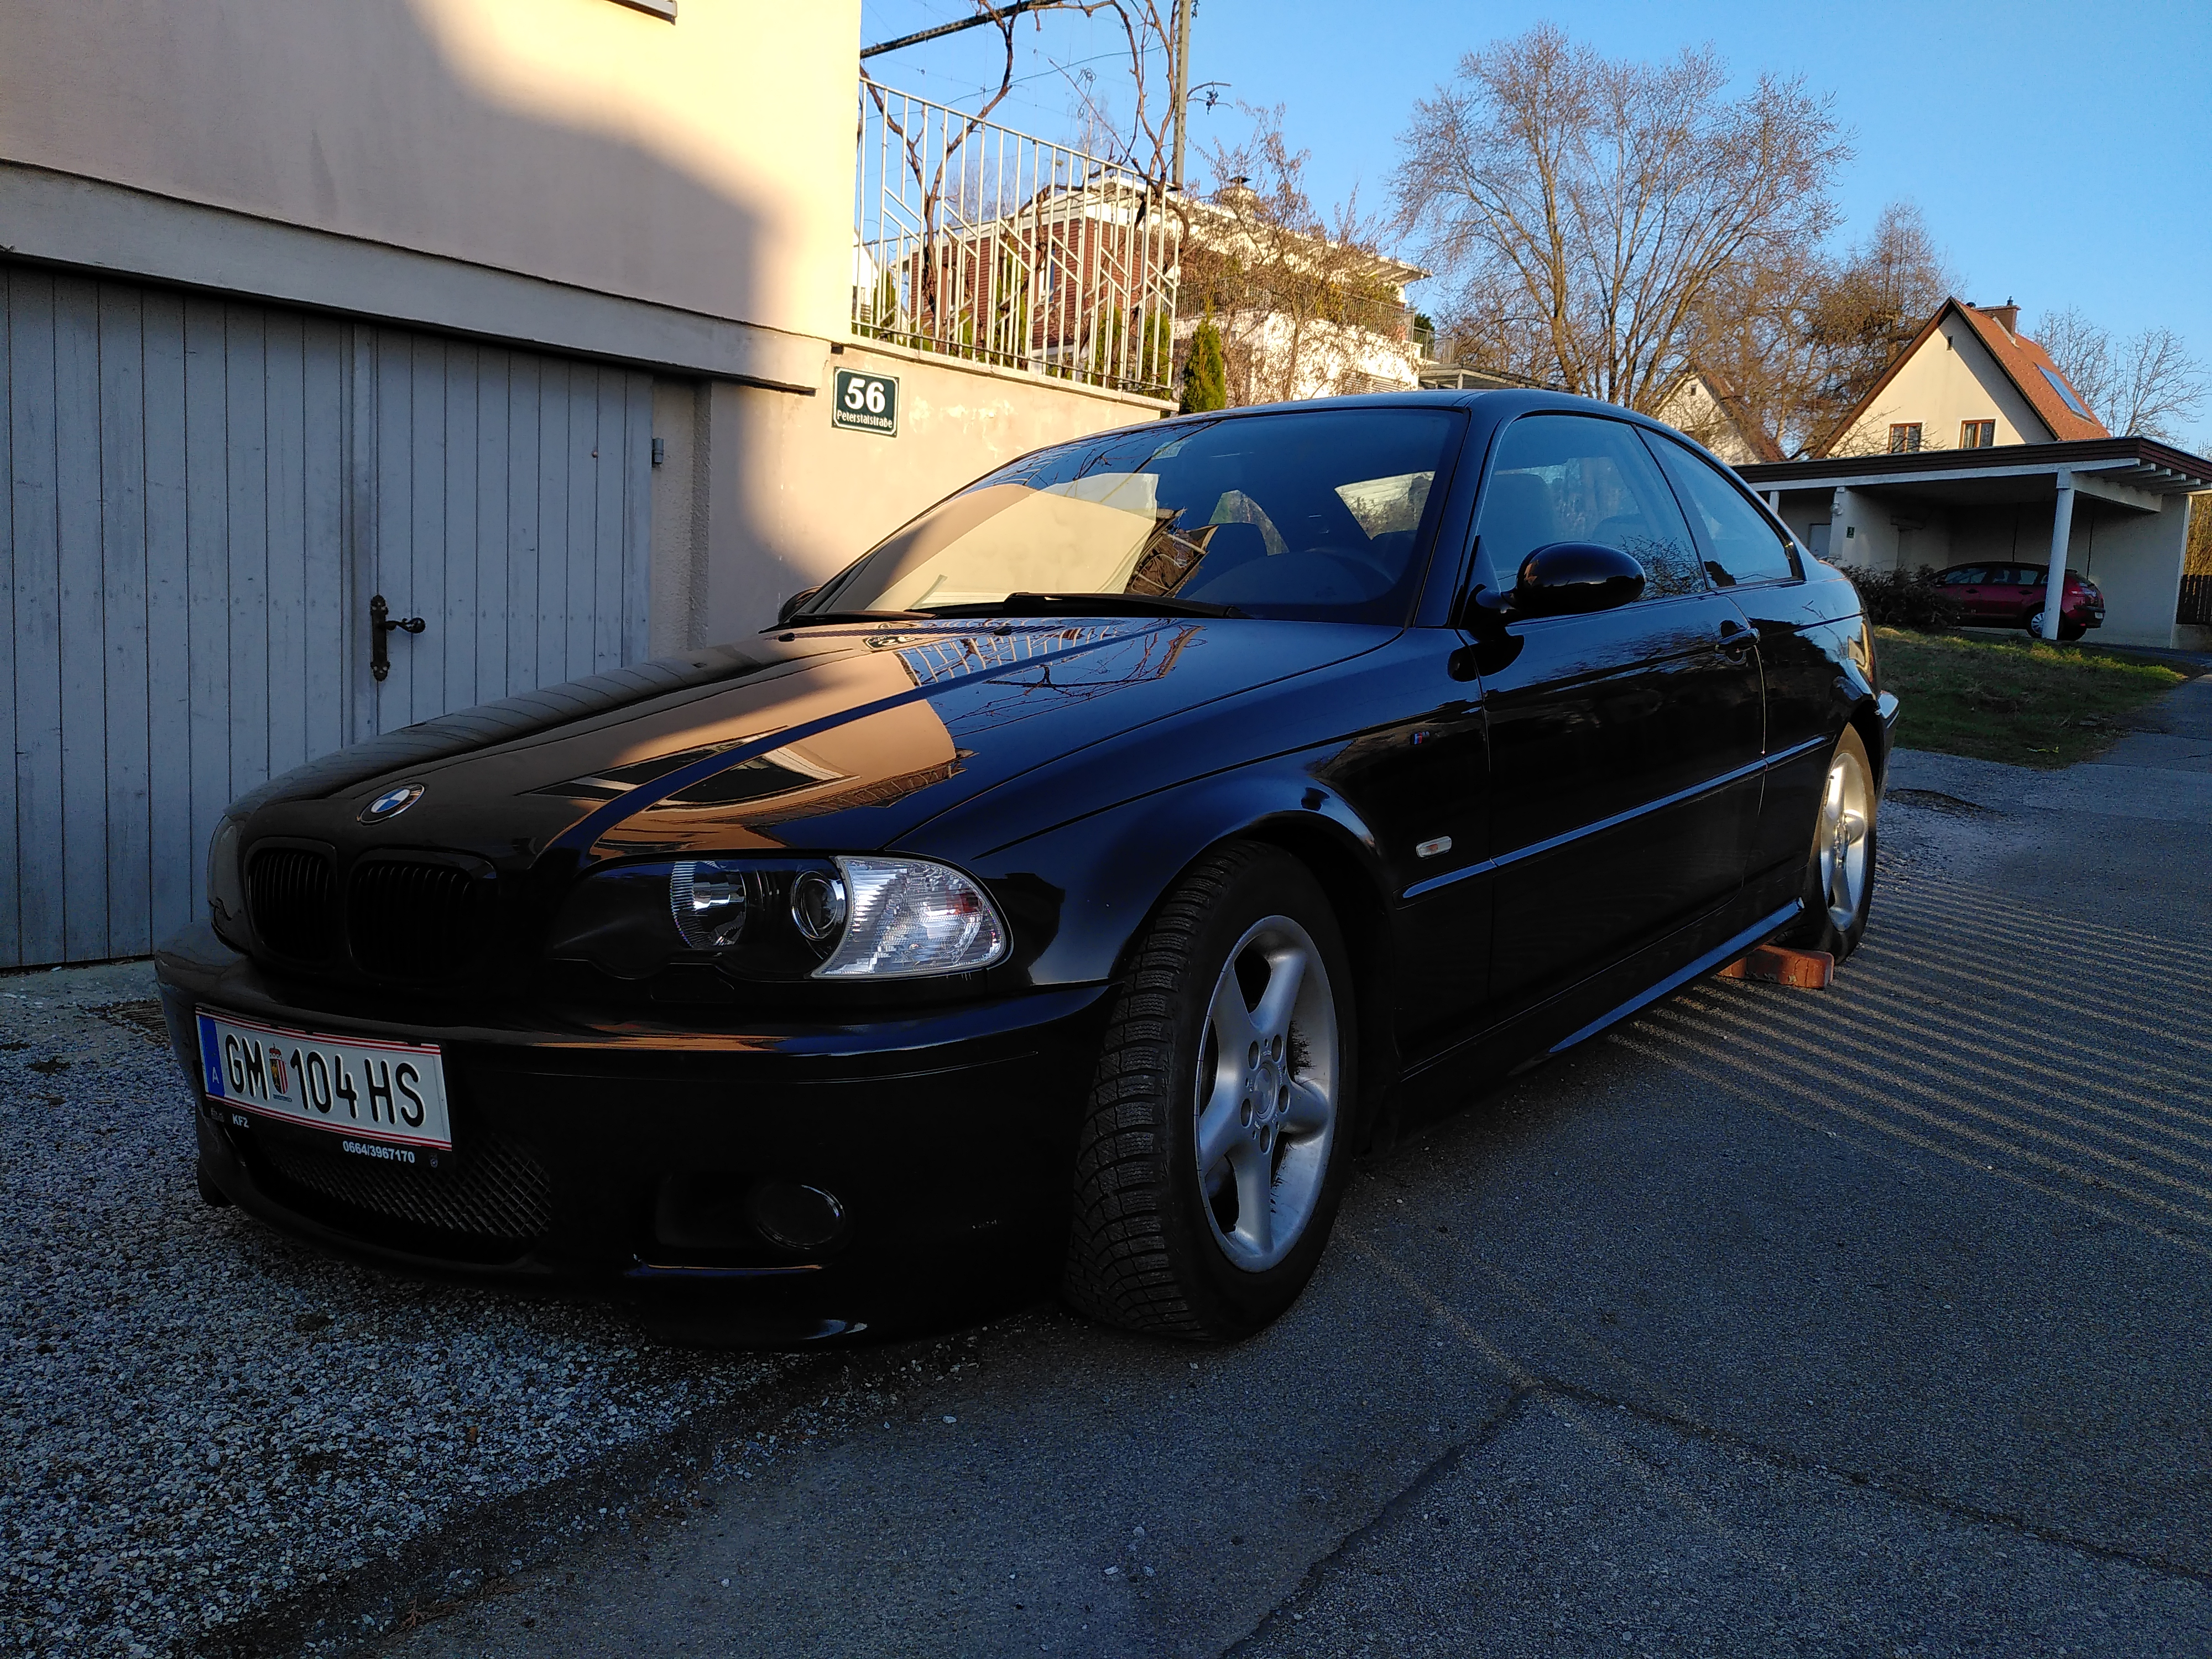
\includegraphics[width=.8\linewidth]{img/demonstration3/vehicle.jpg}
        \caption{The vehicle used for this demonstration}
    \end{center}
\end{figure}

The signal are captured by an ADALM-PLUTO SDR, connected to a laptop running the Open Source Software SDRAngel. This software is released under the OpenGL 3.0+ License and compatible with Windows, OS X as well as many Linux Distributions. It can be donwloaded at the official SDRAngel GitHub repository.\cite{sdrangelgithub}

\begin{figure}[!h]
    \begin{center}
        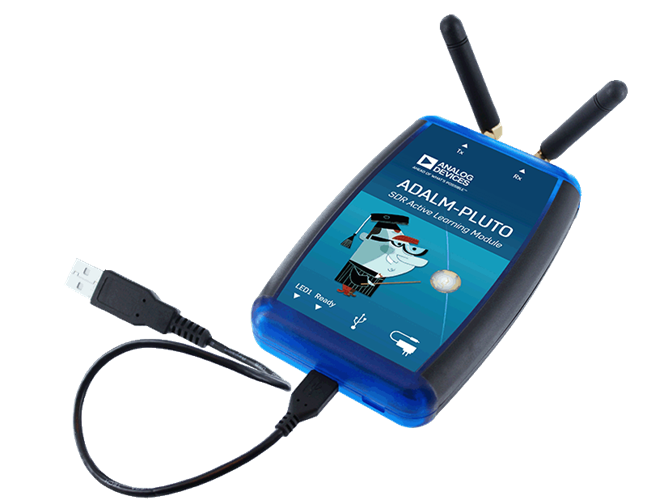
\includegraphics[width=.8\linewidth]{img/demonstration3/ADALM-Pluto-web.png}
        \caption{The SDR used for this demonstration. Source: \cite{adalmphoto}}
    \end{center}
\end{figure}

It will be assumed that the car is parked somewhere with it's doors locked, while the attacker has access to the key, which is in some other location. Presumably it is still in the posession of the victim, which is briefly distracted.

\begin{figure}[!h]
    \begin{center}
        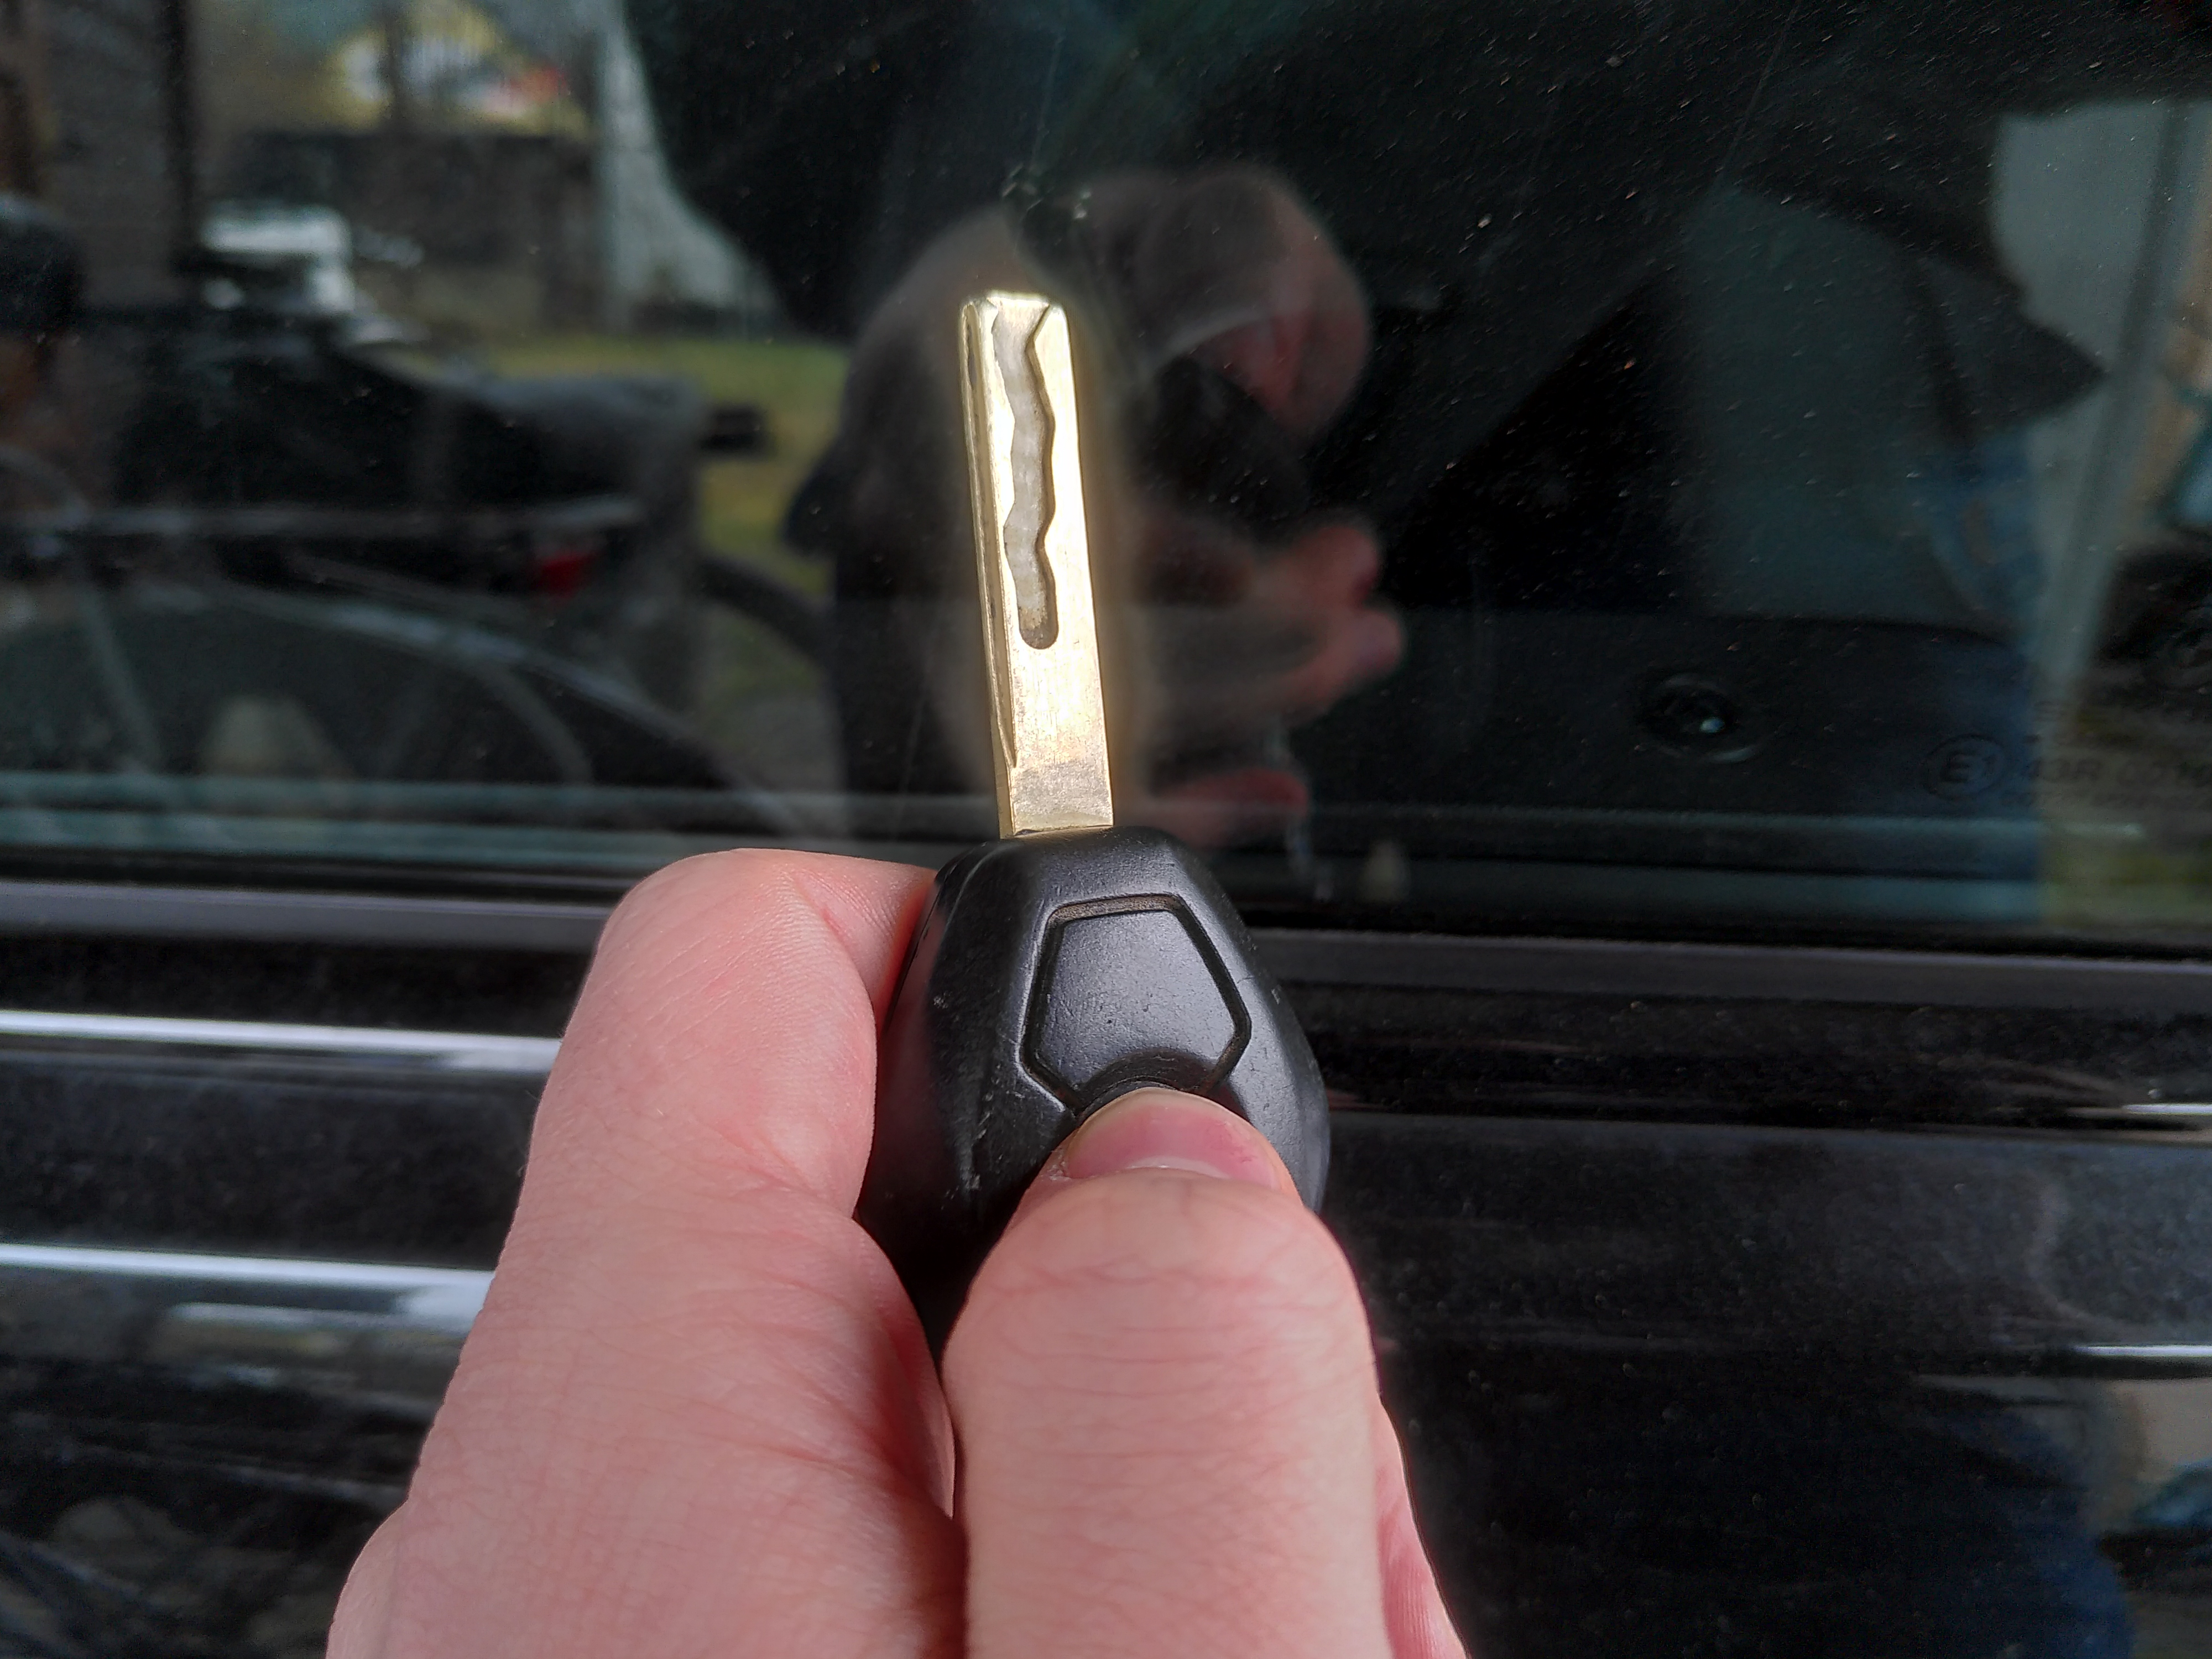
\includegraphics[width=.8\linewidth]{img/demonstration3/locked_door.jpg}
        \caption{The parked vehicle with all doors locked}
    \end{center}
\end{figure}

\subsubsection{Step 1: Set-Up SDR device drivers}
In order to use the SDR on a laptop, the corresponding drivers have to be installed first. This step is heavily dependent on the operating system being used. In Linux, the ADALM-PLUTO should work as a plug and play device out of the box. It is however recommended to install udev rules in order to be able to use the device without root privileges. To do this the corresponding rules have to be downloaded from the Analog Devices website and placed in the following directory:
\begin{verbatim}
    /etc/udev/rules.d/
\end{verbatim}

On a Windows Computer, the drivers can simply be downloaded from the Analog Devices GitHub repository and installed using the graphical installer provided.

\begin{figure}[!h]
    \begin{center}
        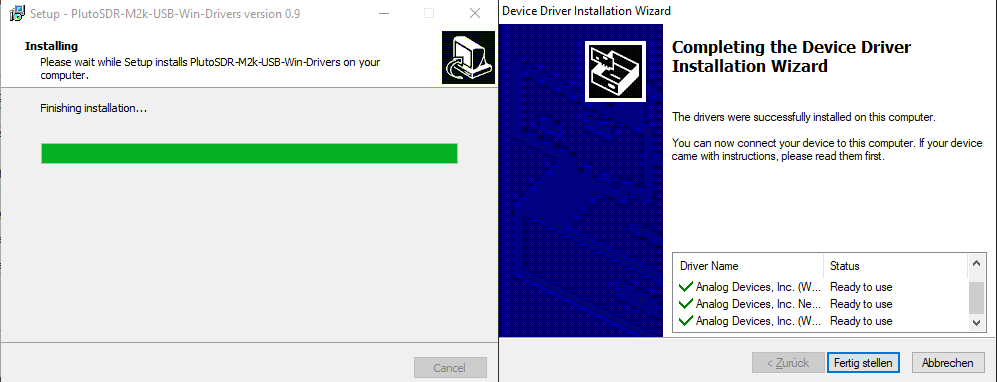
\includegraphics[width=.8\linewidth]{img/demonstration3/driverinstaller.png}
        \caption{The graphical interface for Windows driver installation}
    \end{center}
\end{figure}

\subsubsection{Step 2: Installation of SDRangel}
For illustration purposes, this demo will be performed using a graphical interface, but the ADALM-PLUTO could also be interfaced with from the command line or by writing custom software in C or Python using designated libraries. A number of different programs could be used for this purpose, for example MatLab or Analg Devices' own IIO Oscilloscope. In this demonstration we will use SDRangel. 

SDRangel is a free and open source program developed by Edouard Griffiths originally as an offspring of SDRangelove. It's main purpose is to serve as a GUI frontend for a number of different hardware devices.
Its strength lies in its versatility, because it is organized into workspaces on which devices can be arranged to fit innumerable use cases.
There are a number of plugins provided with the software, which makes it possible to use many different devices out of the box and use features like file recording and playback.\cite{sdrangelgit}
The software can be downloaded from the respective GitHub repository and is available for a number of different platforms including Windows, OS X and Linux. It is also available in the package manager repositories.

\subsubsection{Step 3: Configuring the SDRangel workspace}

Once the program is installed successfully and launched, the user is greated with an empty canvas on which UI-elements and plugins need to be created to fit the desired purpose. This is done by first creating the device necessary. Since the ADALM-PLUTO can receive and transmit signals at the same time, it can be created as a ``Multiple-Input Multiple-Output (MIMO)'' device. There is a corresponding button in the toolbar of the GUI. 

\begin{figure}[!h]
    \begin{center}
        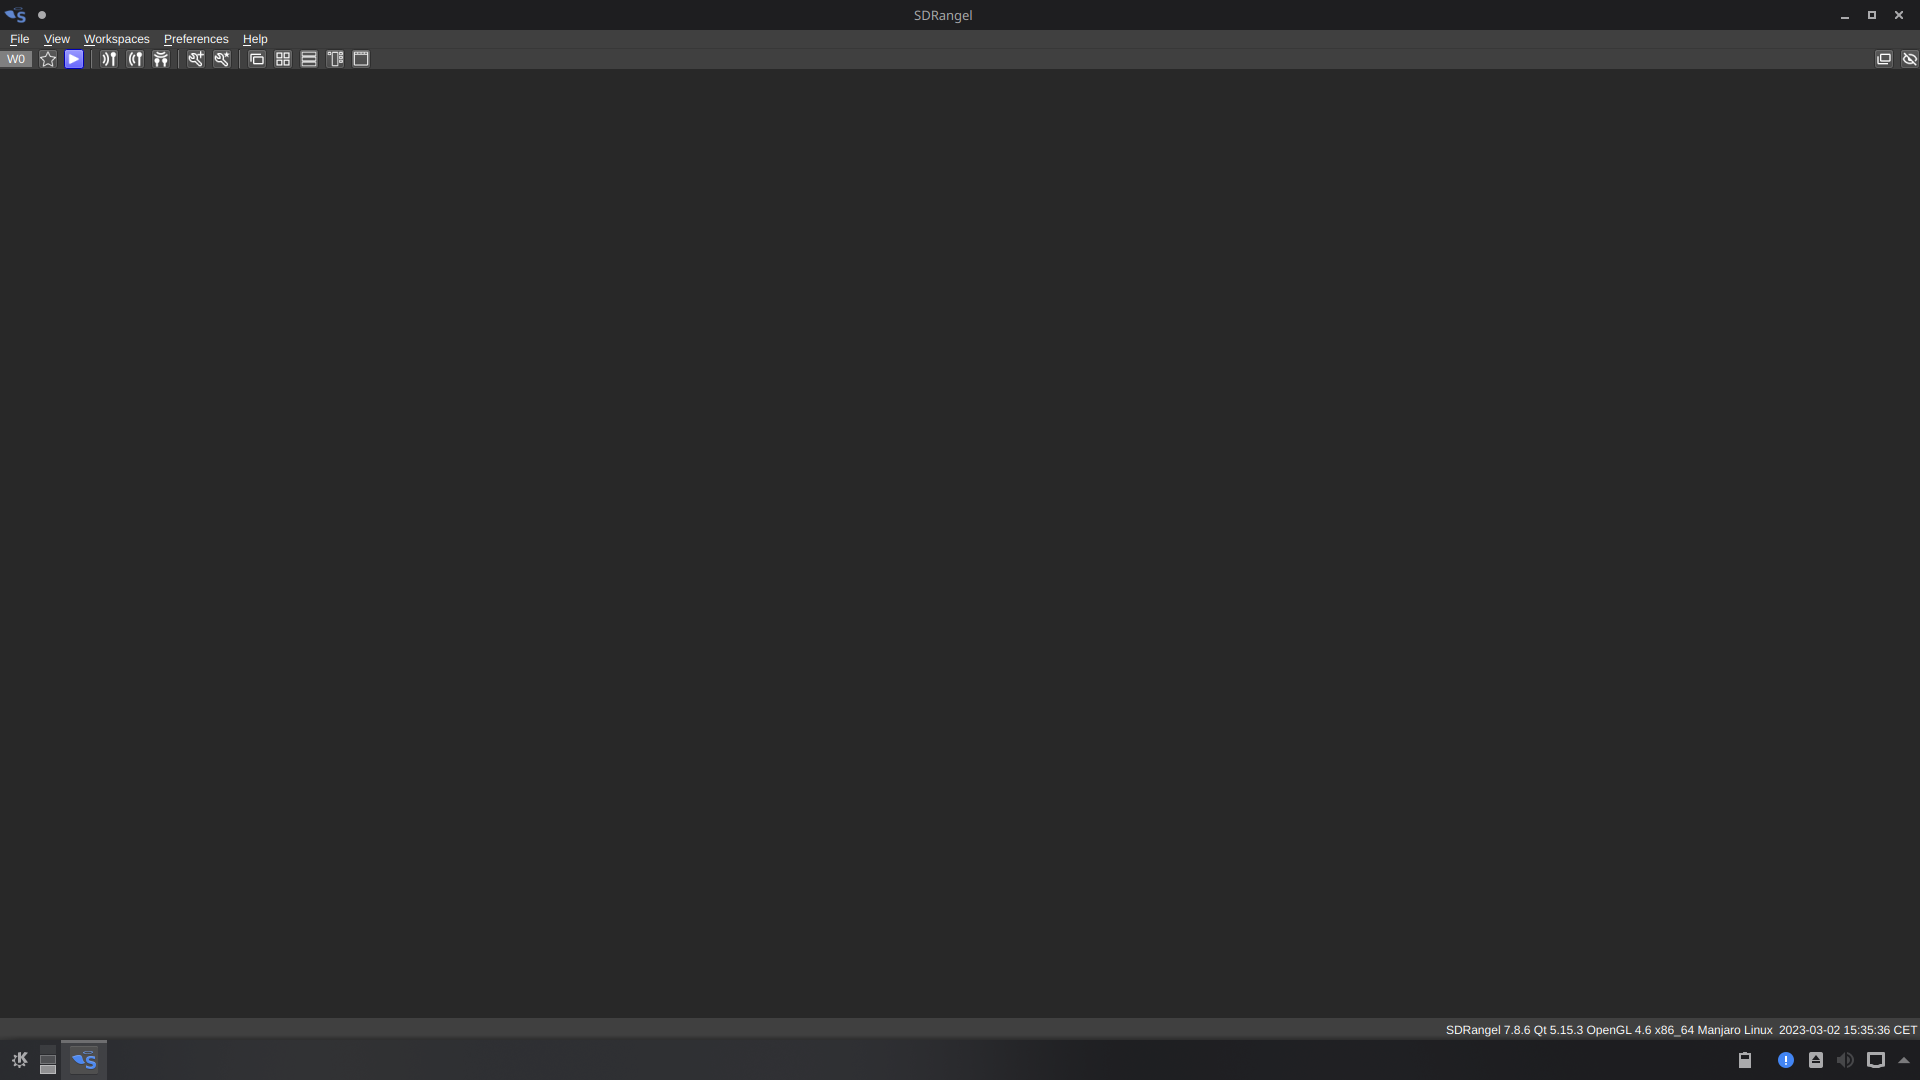
\includegraphics[width=.8\linewidth]{img/demonstration3/empty_canvas.png}
        \caption{SDRangel on first startup showing an empty workspace}
    \end{center}
\end{figure}

After pressing this button, the program asks the user to select the desired sampling device. As the ADALM-PLUTO is supported out of the box and the drivers were previously installed, it should already appear in this drop-down menu.

\begin{figure}[!h]
    \begin{center}
        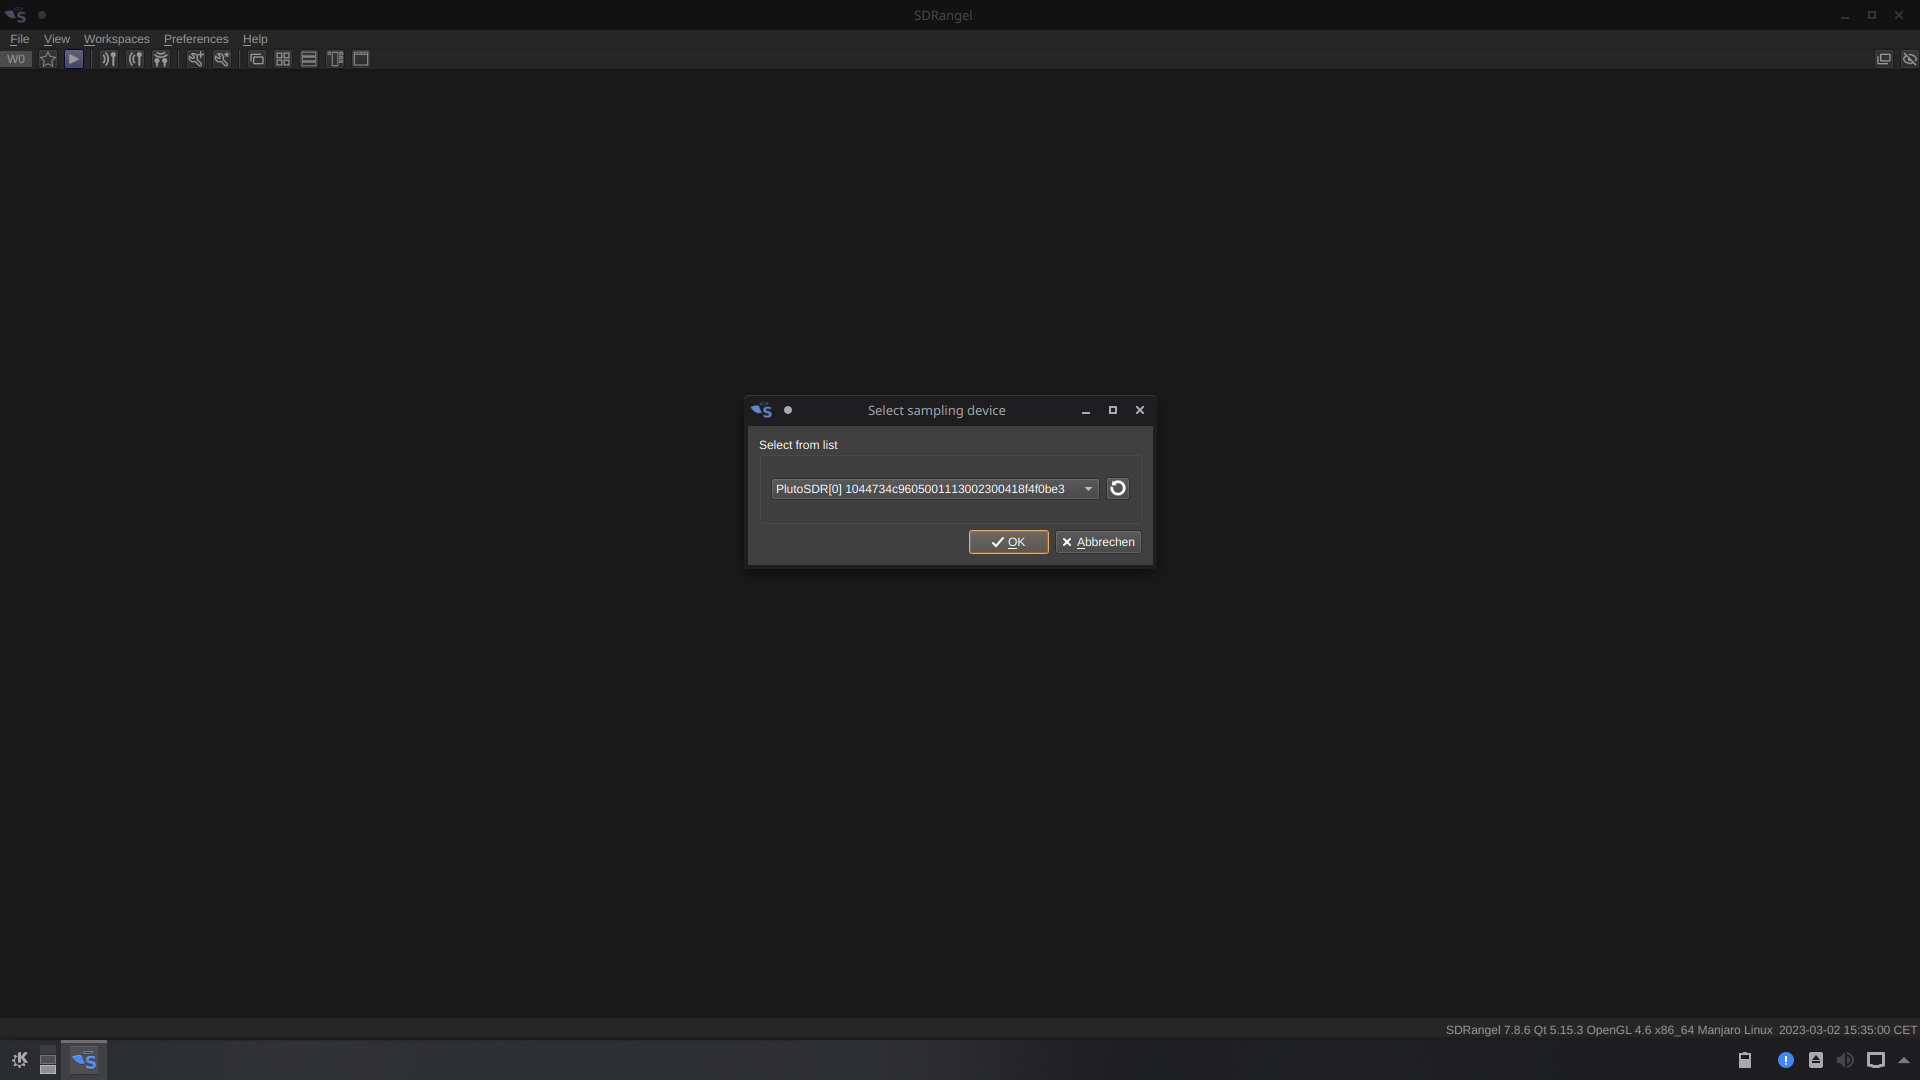
\includegraphics[width=.8\linewidth]{img/demonstration3/new_device.png}
        \caption{The dropdown of available devices after clicking on ``New MIMO device''}
    \end{center}
\end{figure}

Now two windows appear in the workspace: 
The first is a spectogram plotting the signals in the frequency spectrum the device is currently transmitting on.
The second is a control panel in which the `acquisition' and `generation' (also known as the transmission and reception) of signals can be turned on or off and the corresponding frequency can be set. A number of other software and hardware features like DC component removal and imbalance correction can also be turned on or off here, but these are irrelevant for the demonstration. The last important UI elemnt in this window is a button to add more channels to this device. This can be used to enable recording to a file as well as transmitting a signal that was previously saved to a device.

\begin{figure}[!h]
    \begin{center}
        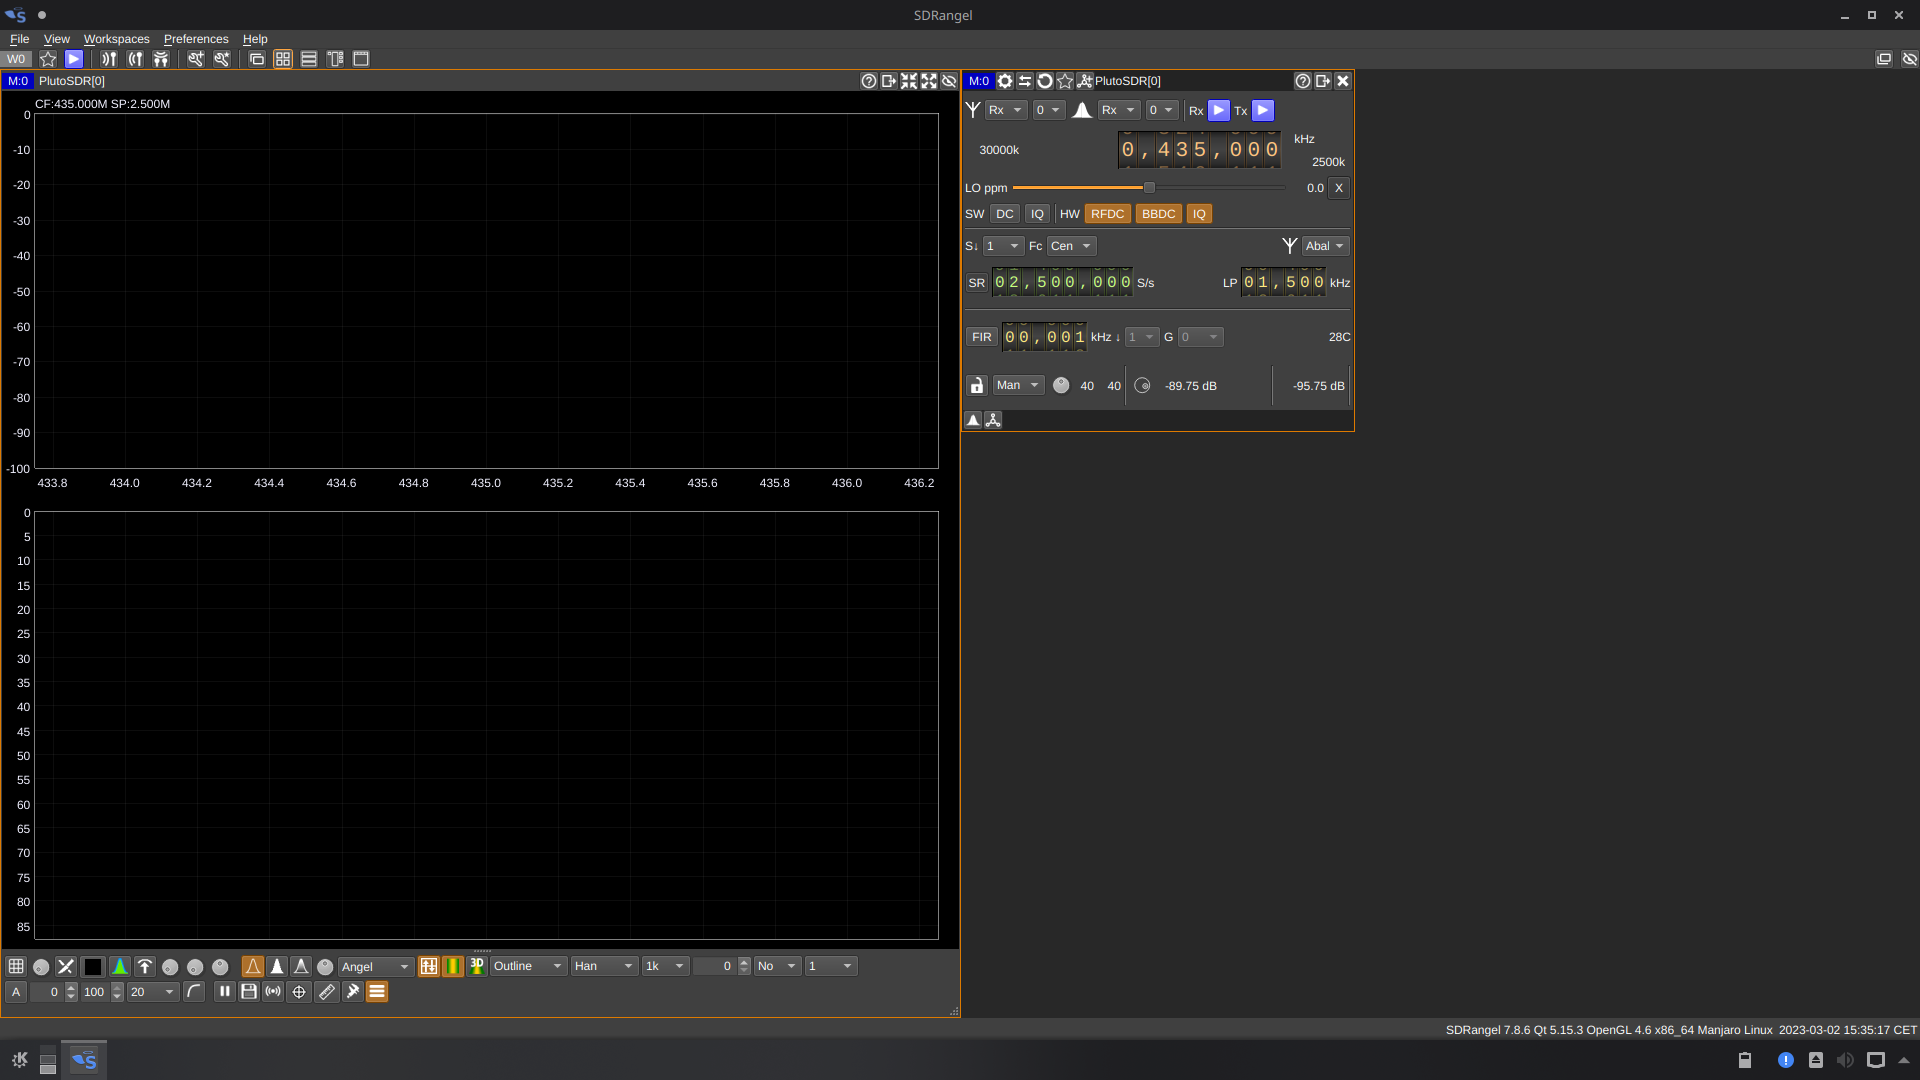
\includegraphics[width=.8\linewidth]{img/demonstration3/new_device2.png}
        \caption{Spectogram and control panel of the new device}
    \end{center}
\end{figure}


When this button is clicked, a drop-down element occurs listing all the currently available plugins for this device. For this demonstration ``File Sink'' and ``File Channel Source'' windows need to be added, before this dialogue box can be closed again. The finished workspace looks like shown in figure \ref{fig:addchannel}.

\begin{figure}[!h]
    \begin{center}
        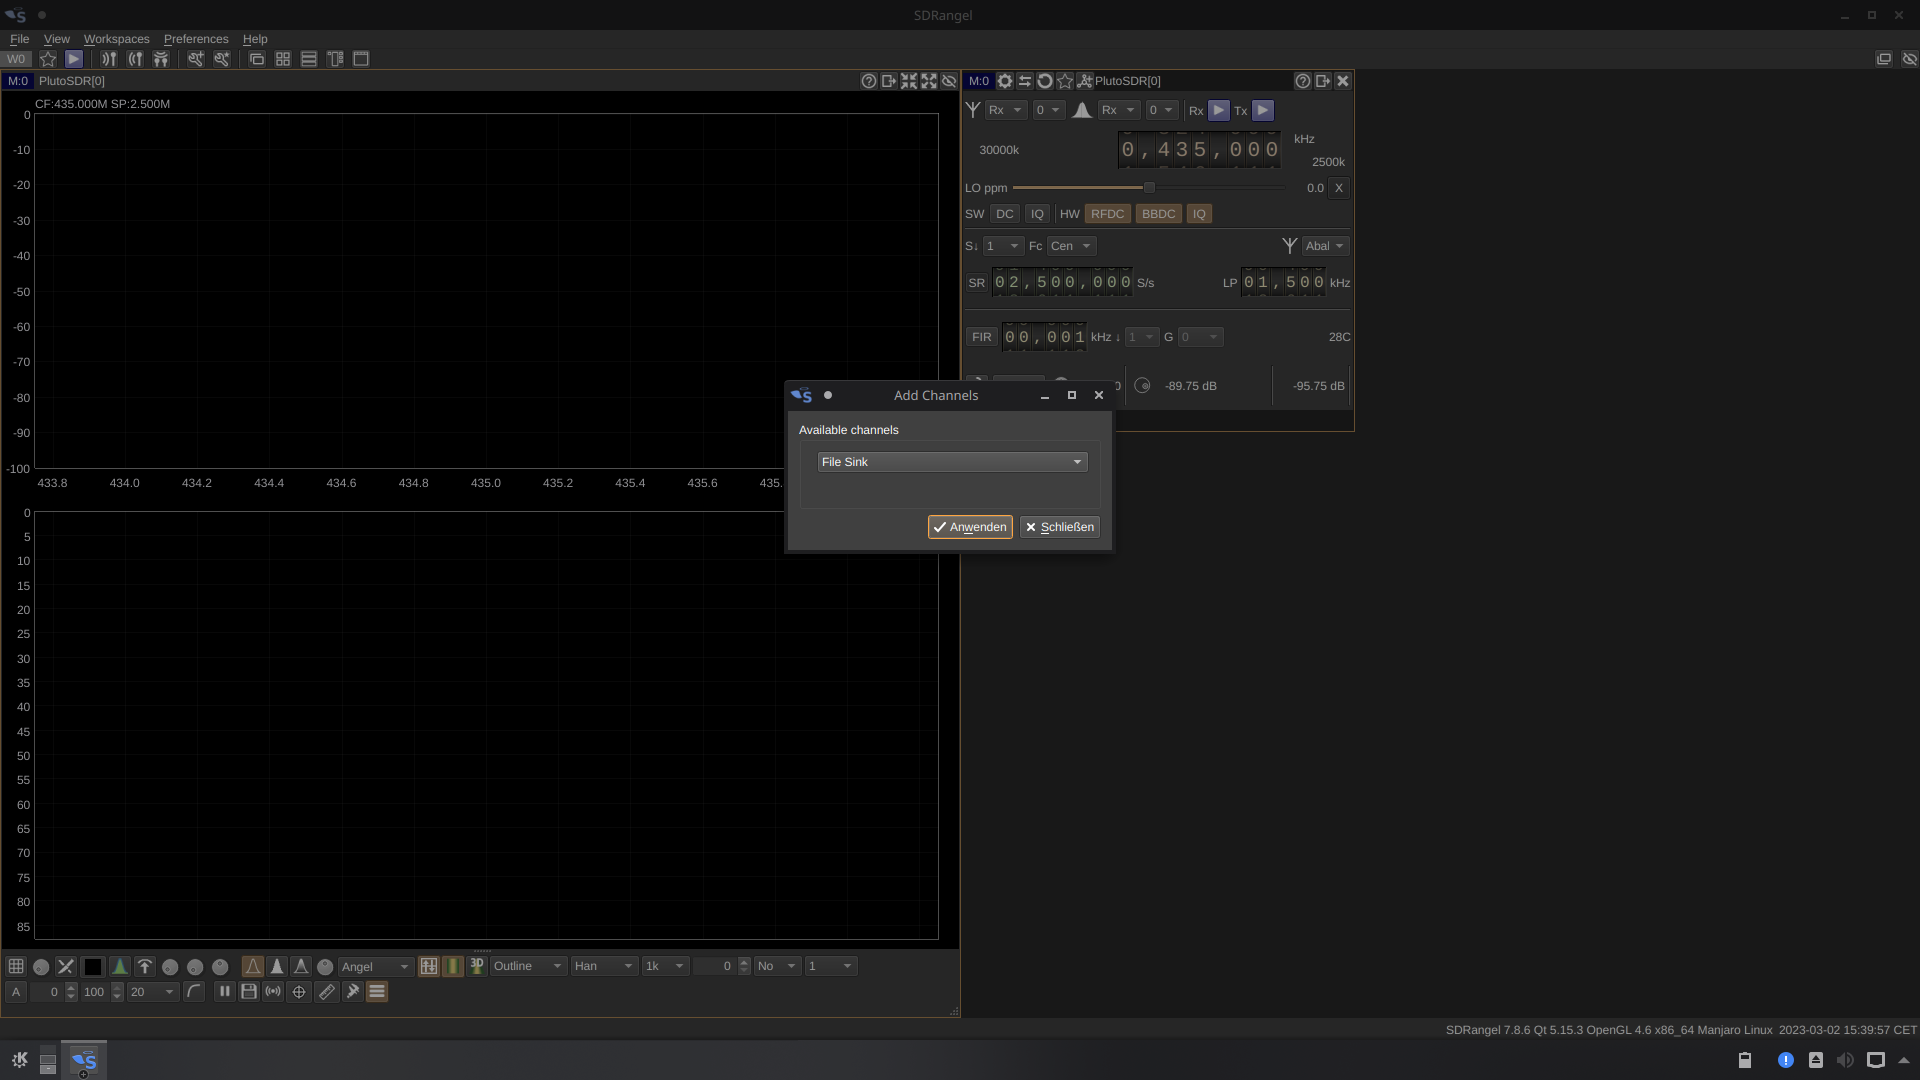
\includegraphics[width=.8\linewidth]{img/demonstration3/new_channel.png}
        \caption{Adding the ``File Sink'' and ``File channel source'' channels}
        \label{fig:addchannel}
    \end{center}
\end{figure}

The finished workspace can be seen in figure \ref{fig:finishedworkspace}:

\begin{figure}[!h]
    \begin{center}
        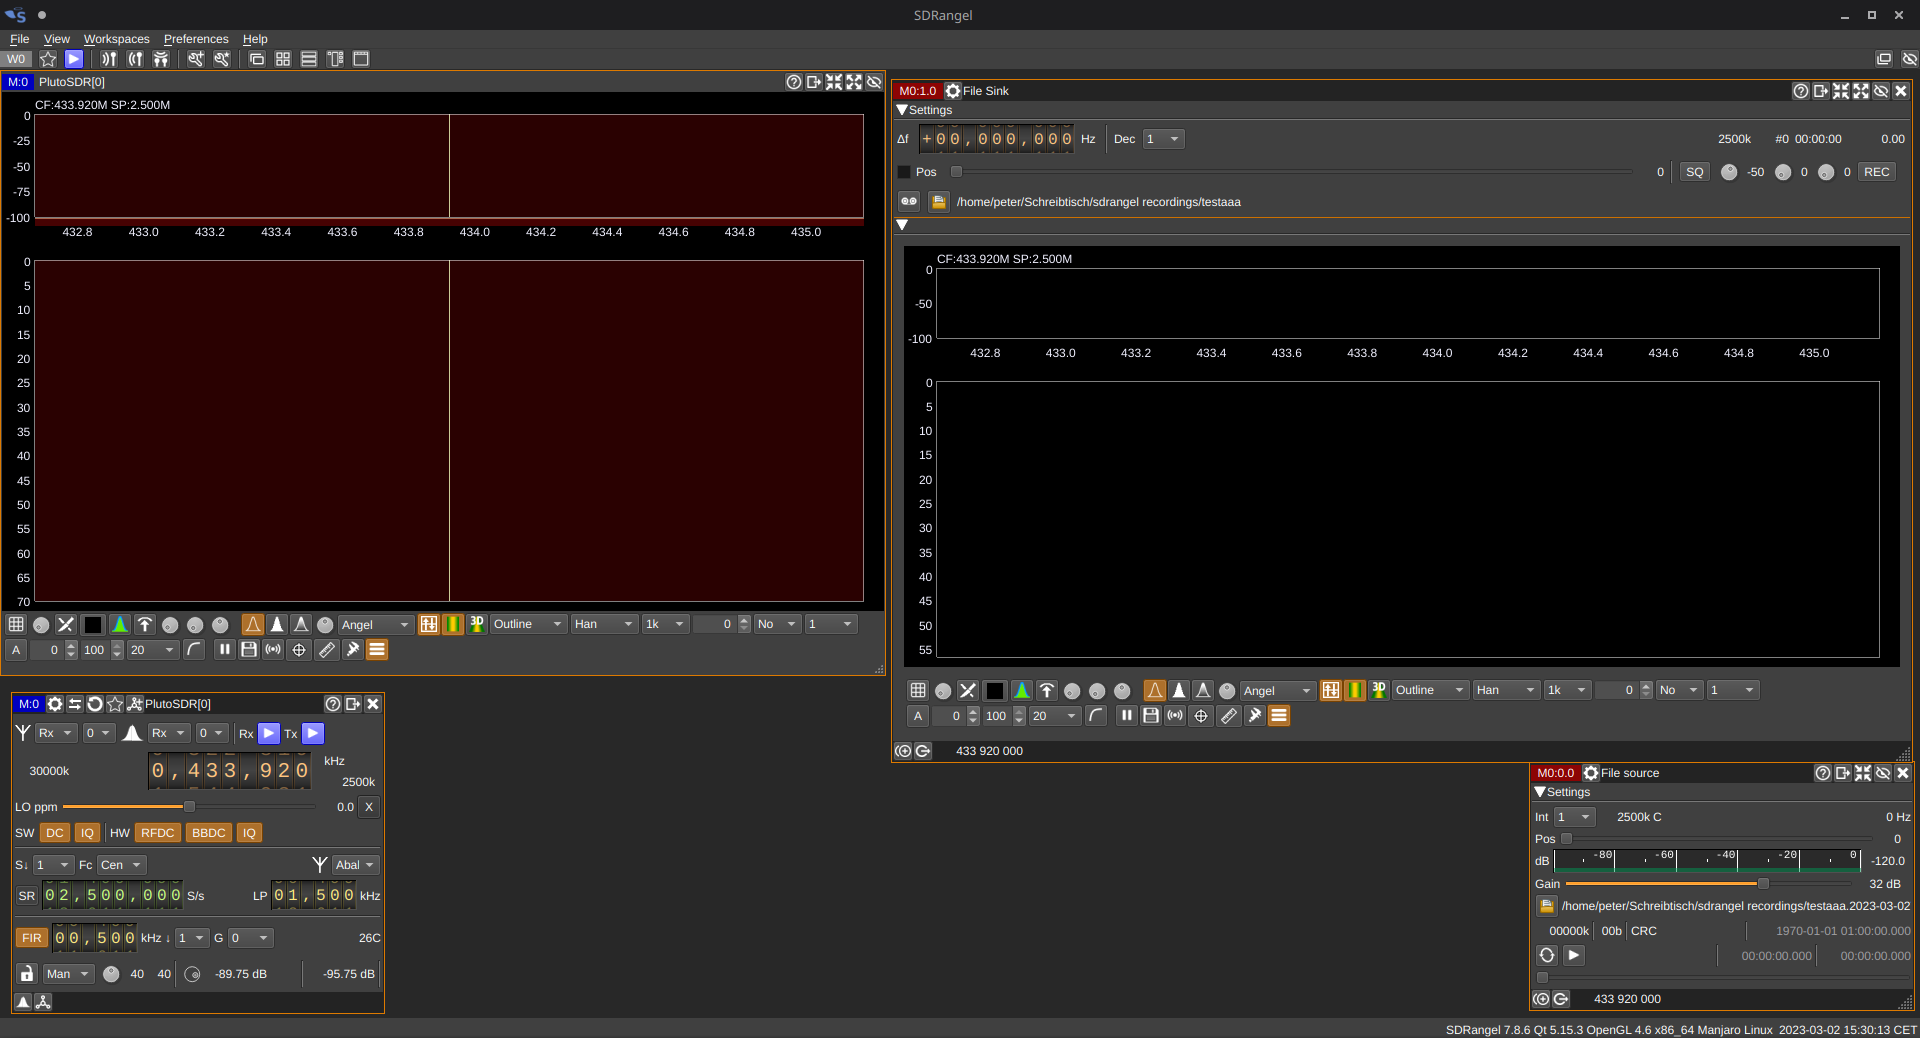
\includegraphics[width=.8\linewidth]{img/demonstration3/finished workspace.png}
        \caption{The finished workspace}
        \label{fig:finishedworkspace}
    \end{center}
\end{figure}

\subsubsection{Step 4: Capturing an unlock signal}
Once the workspace is set up as described above, the RFID unlock signal can be captured. To do so, the SDR needs to be configured to transmit on a frequency of 433,92MHz, as this is the frequency at which this particular key fob sends it's signals. This is accomplished via the ``Main center frequency'' text box.

The path to which the file will be saved can be set via the ``Open file'' dialogue. When all necessary options are set, the acquisition of signals can be started by clicking the corresponding ``Rx'' button. The ``Start/Stop recording'' button can then be used to start capturing. At this point the key can be positioned close to the devices' antennas and a open keypress can be recorded. Once finished, the same button is used to stop the recording. After that, the Rx button can also be deactivated.

\begin{figure}[!h]
    \begin{center}
        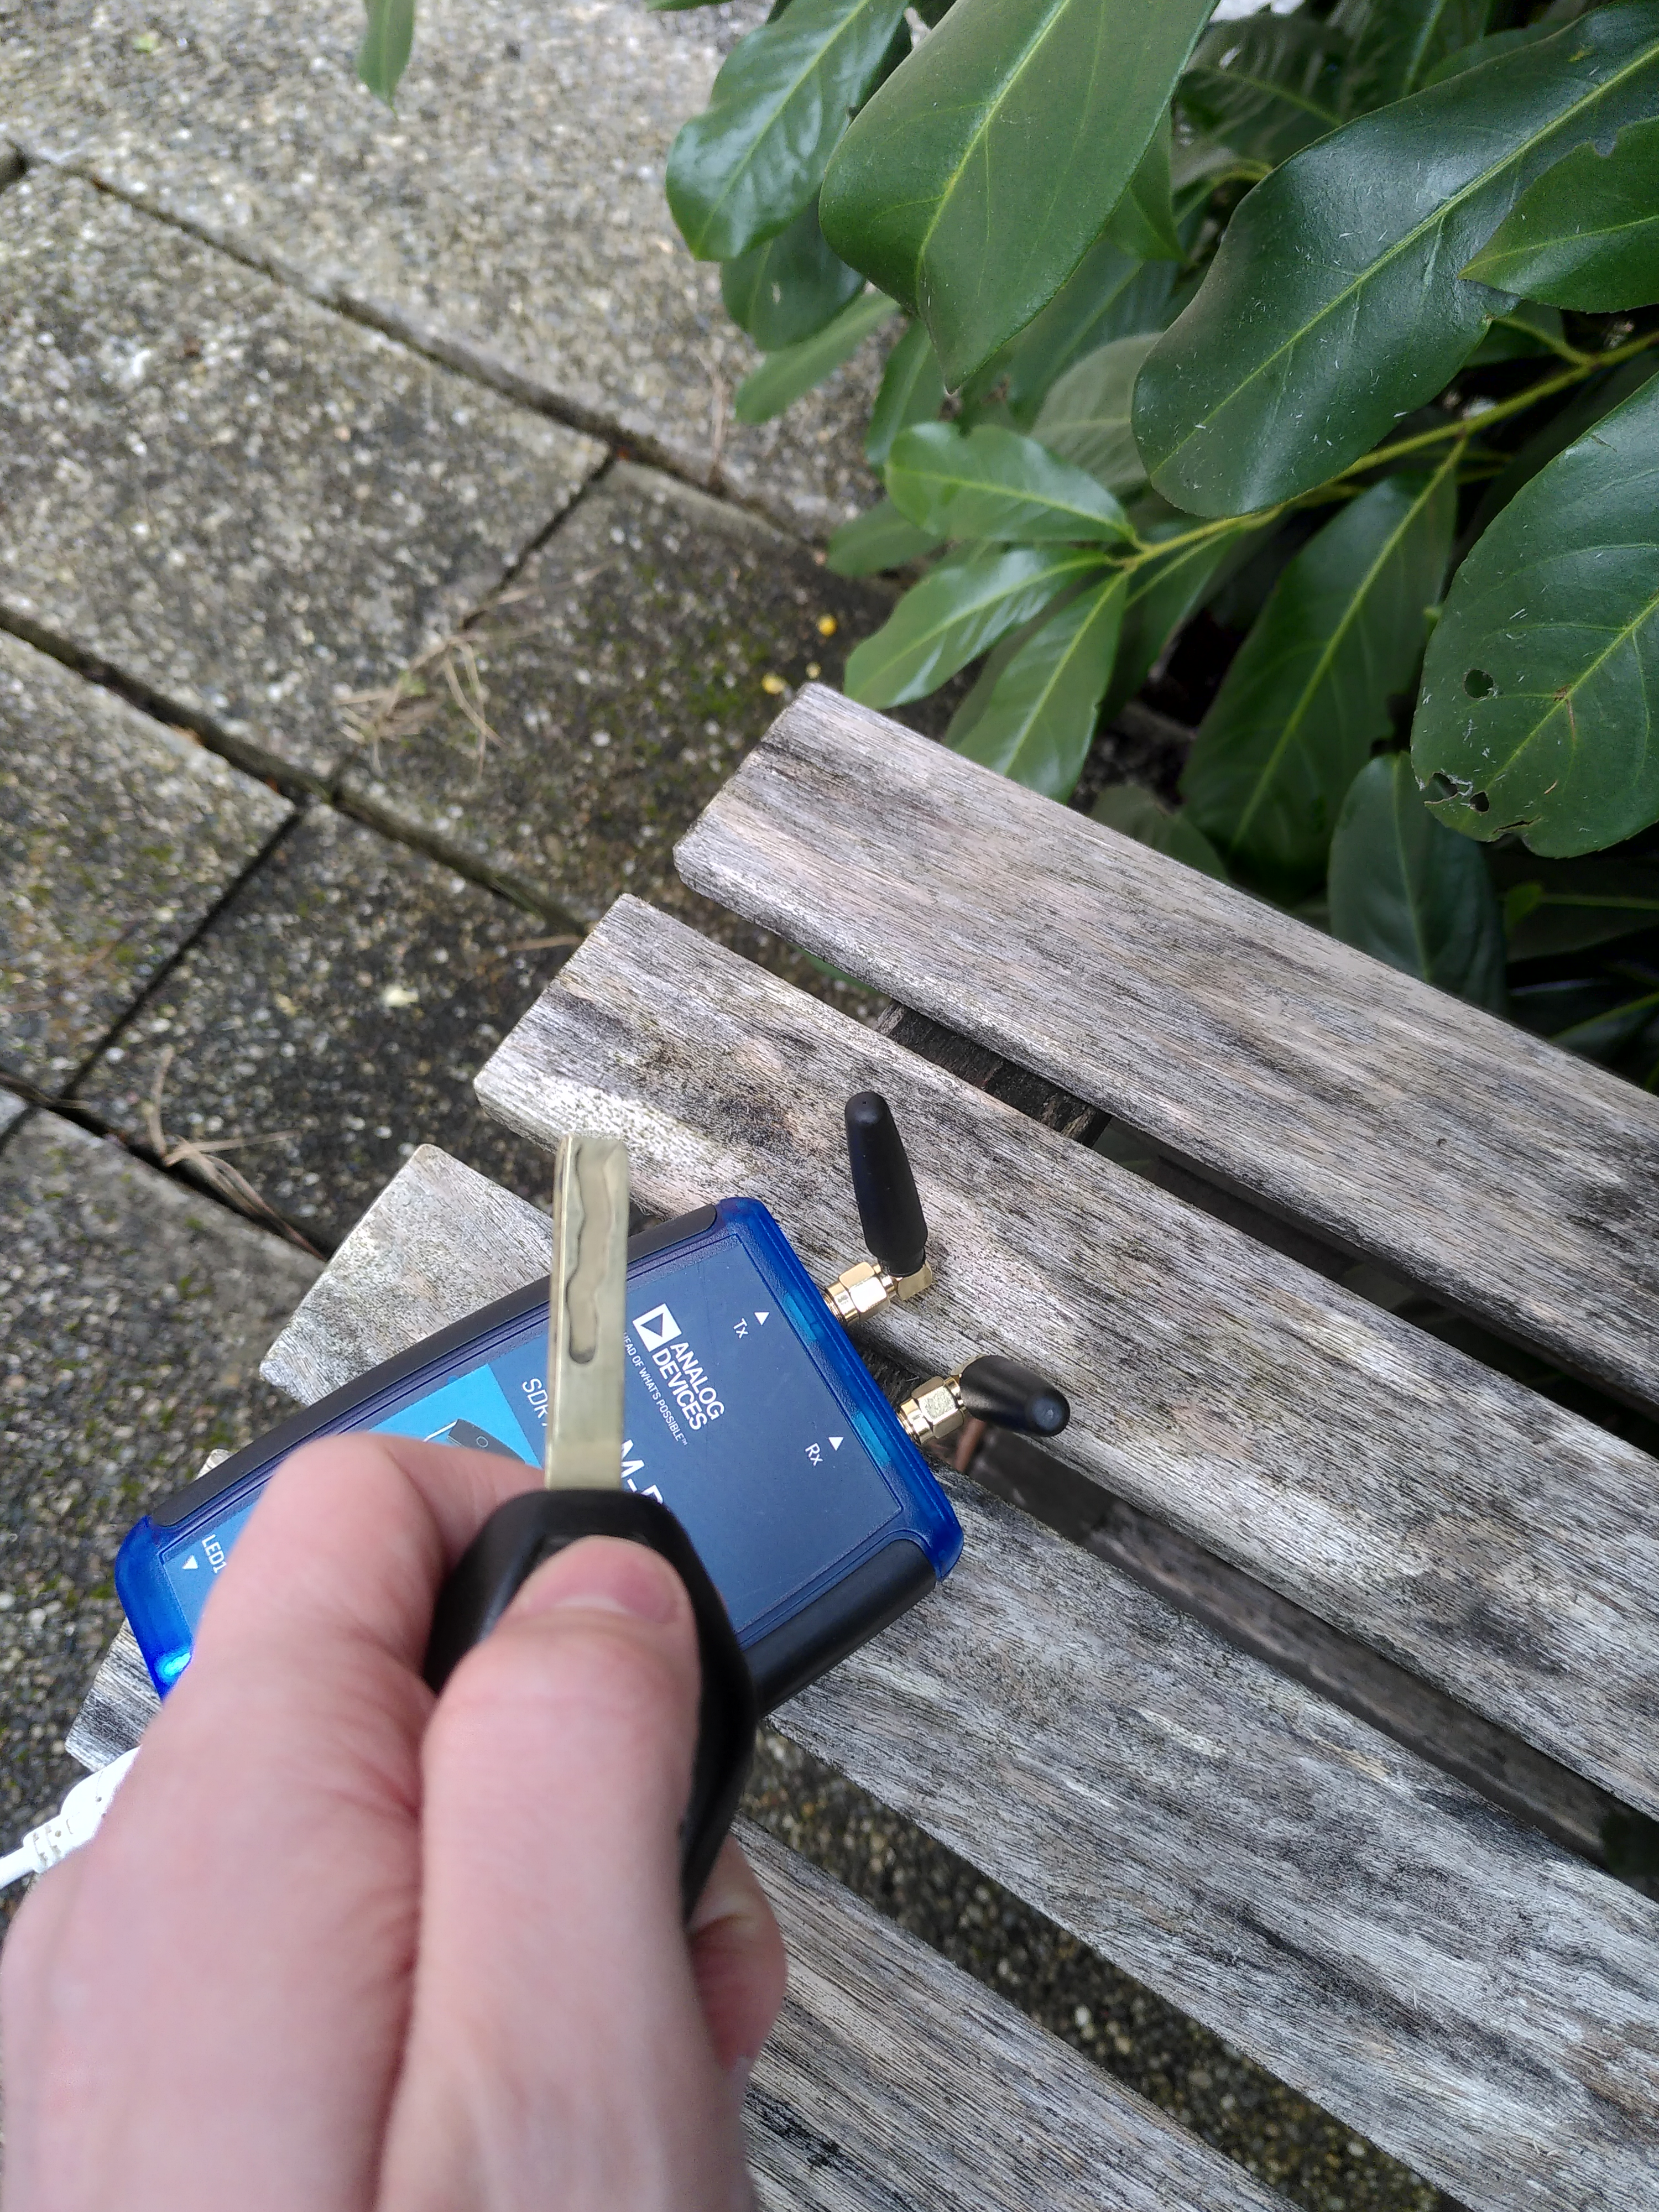
\includegraphics[width=.8\linewidth]{img/demonstration3/signal_capture_key_placement.jpg}
        \caption{SDRangel while capturing the signal}
    \end{center}
\end{figure}

It is important that the Attack only works if the signal of the key does not reach the car, since this would cause the code to be rolled over to the next iteration, rendering the captured signal useless.

\begin{figure}[!h]
    \begin{center}
        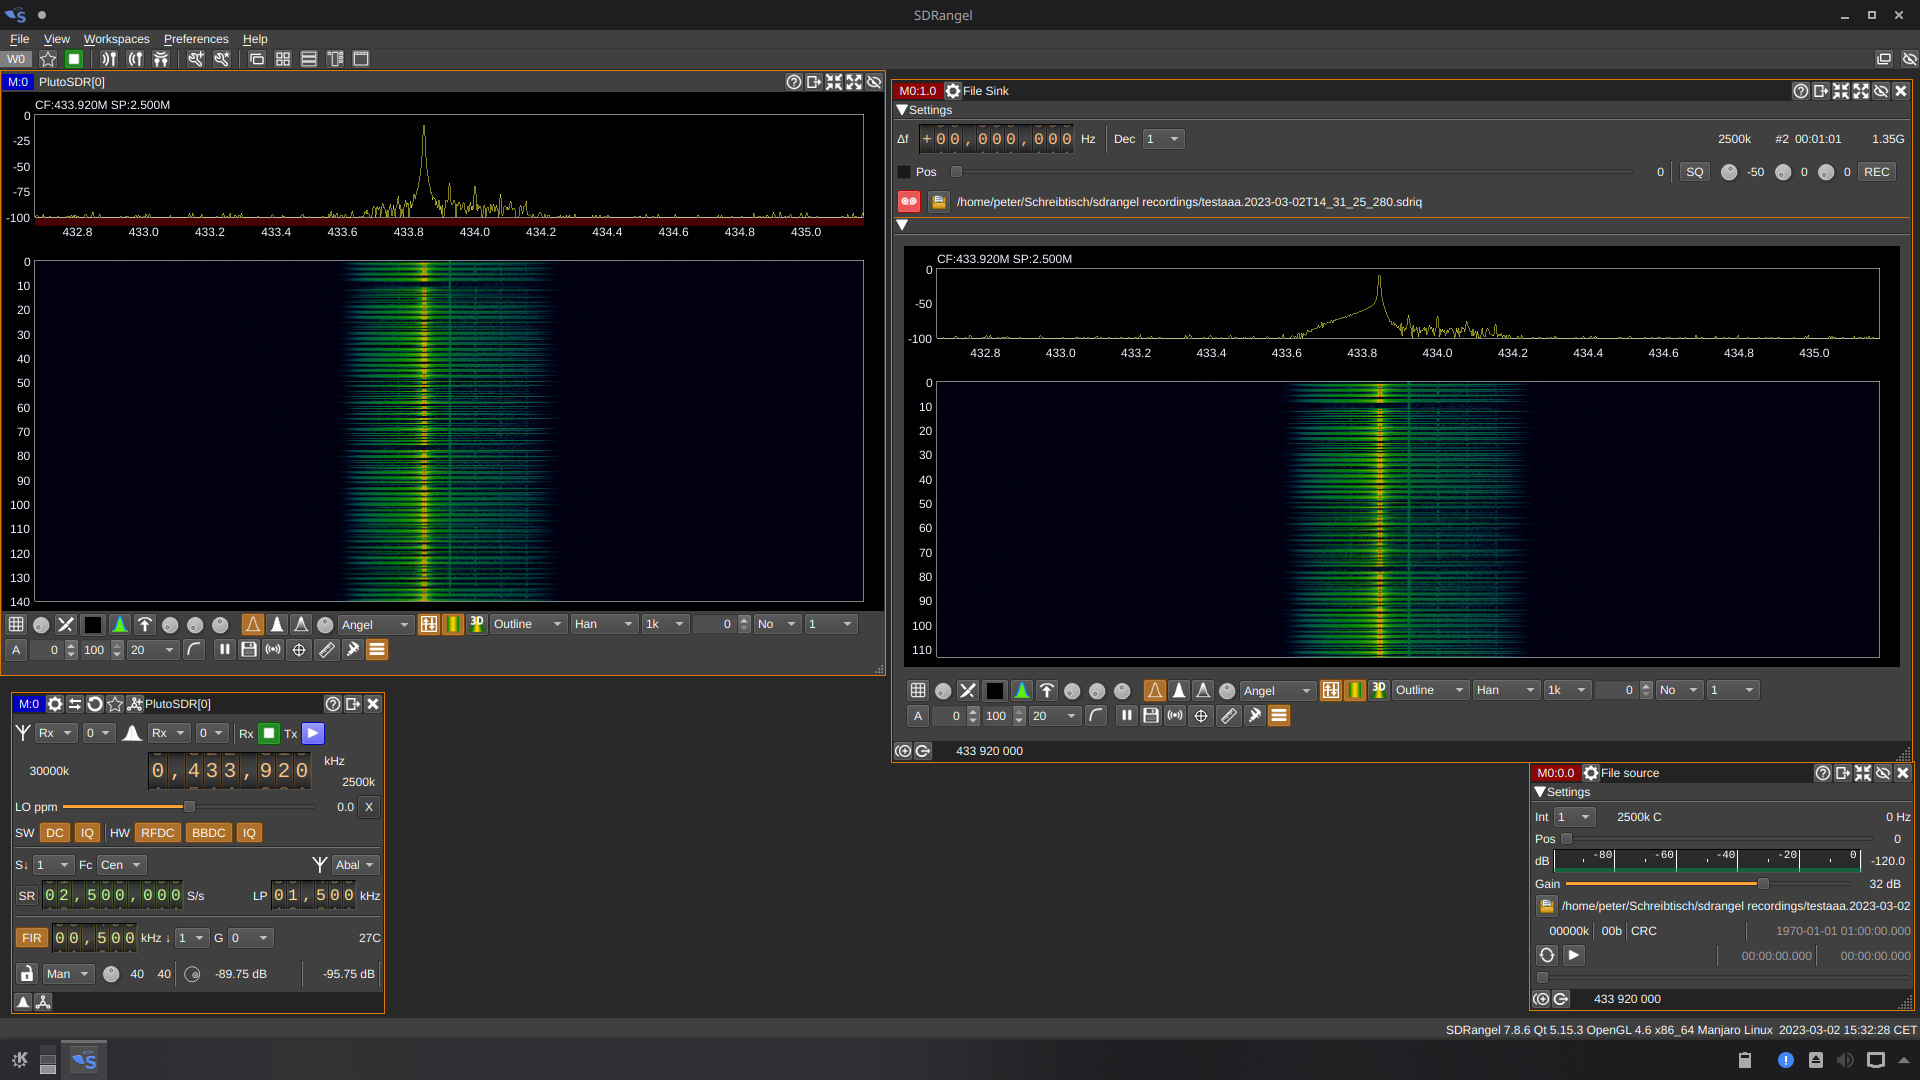
\includegraphics[width=.8\linewidth]{img/demonstration3/capturing_signal.png}
        \caption{SDRangel while capturing the signal}
    \end{center}
\end{figure}

\subsubsection{Step 5: Playing back the signal near the vehicle}

In order to actually use the signal, the host computer with the connected SDR should now be moved close to the vehicle. The key is no longer necessary to be present for the following steps.


\begin{figure}[!h]
    \begin{center}
        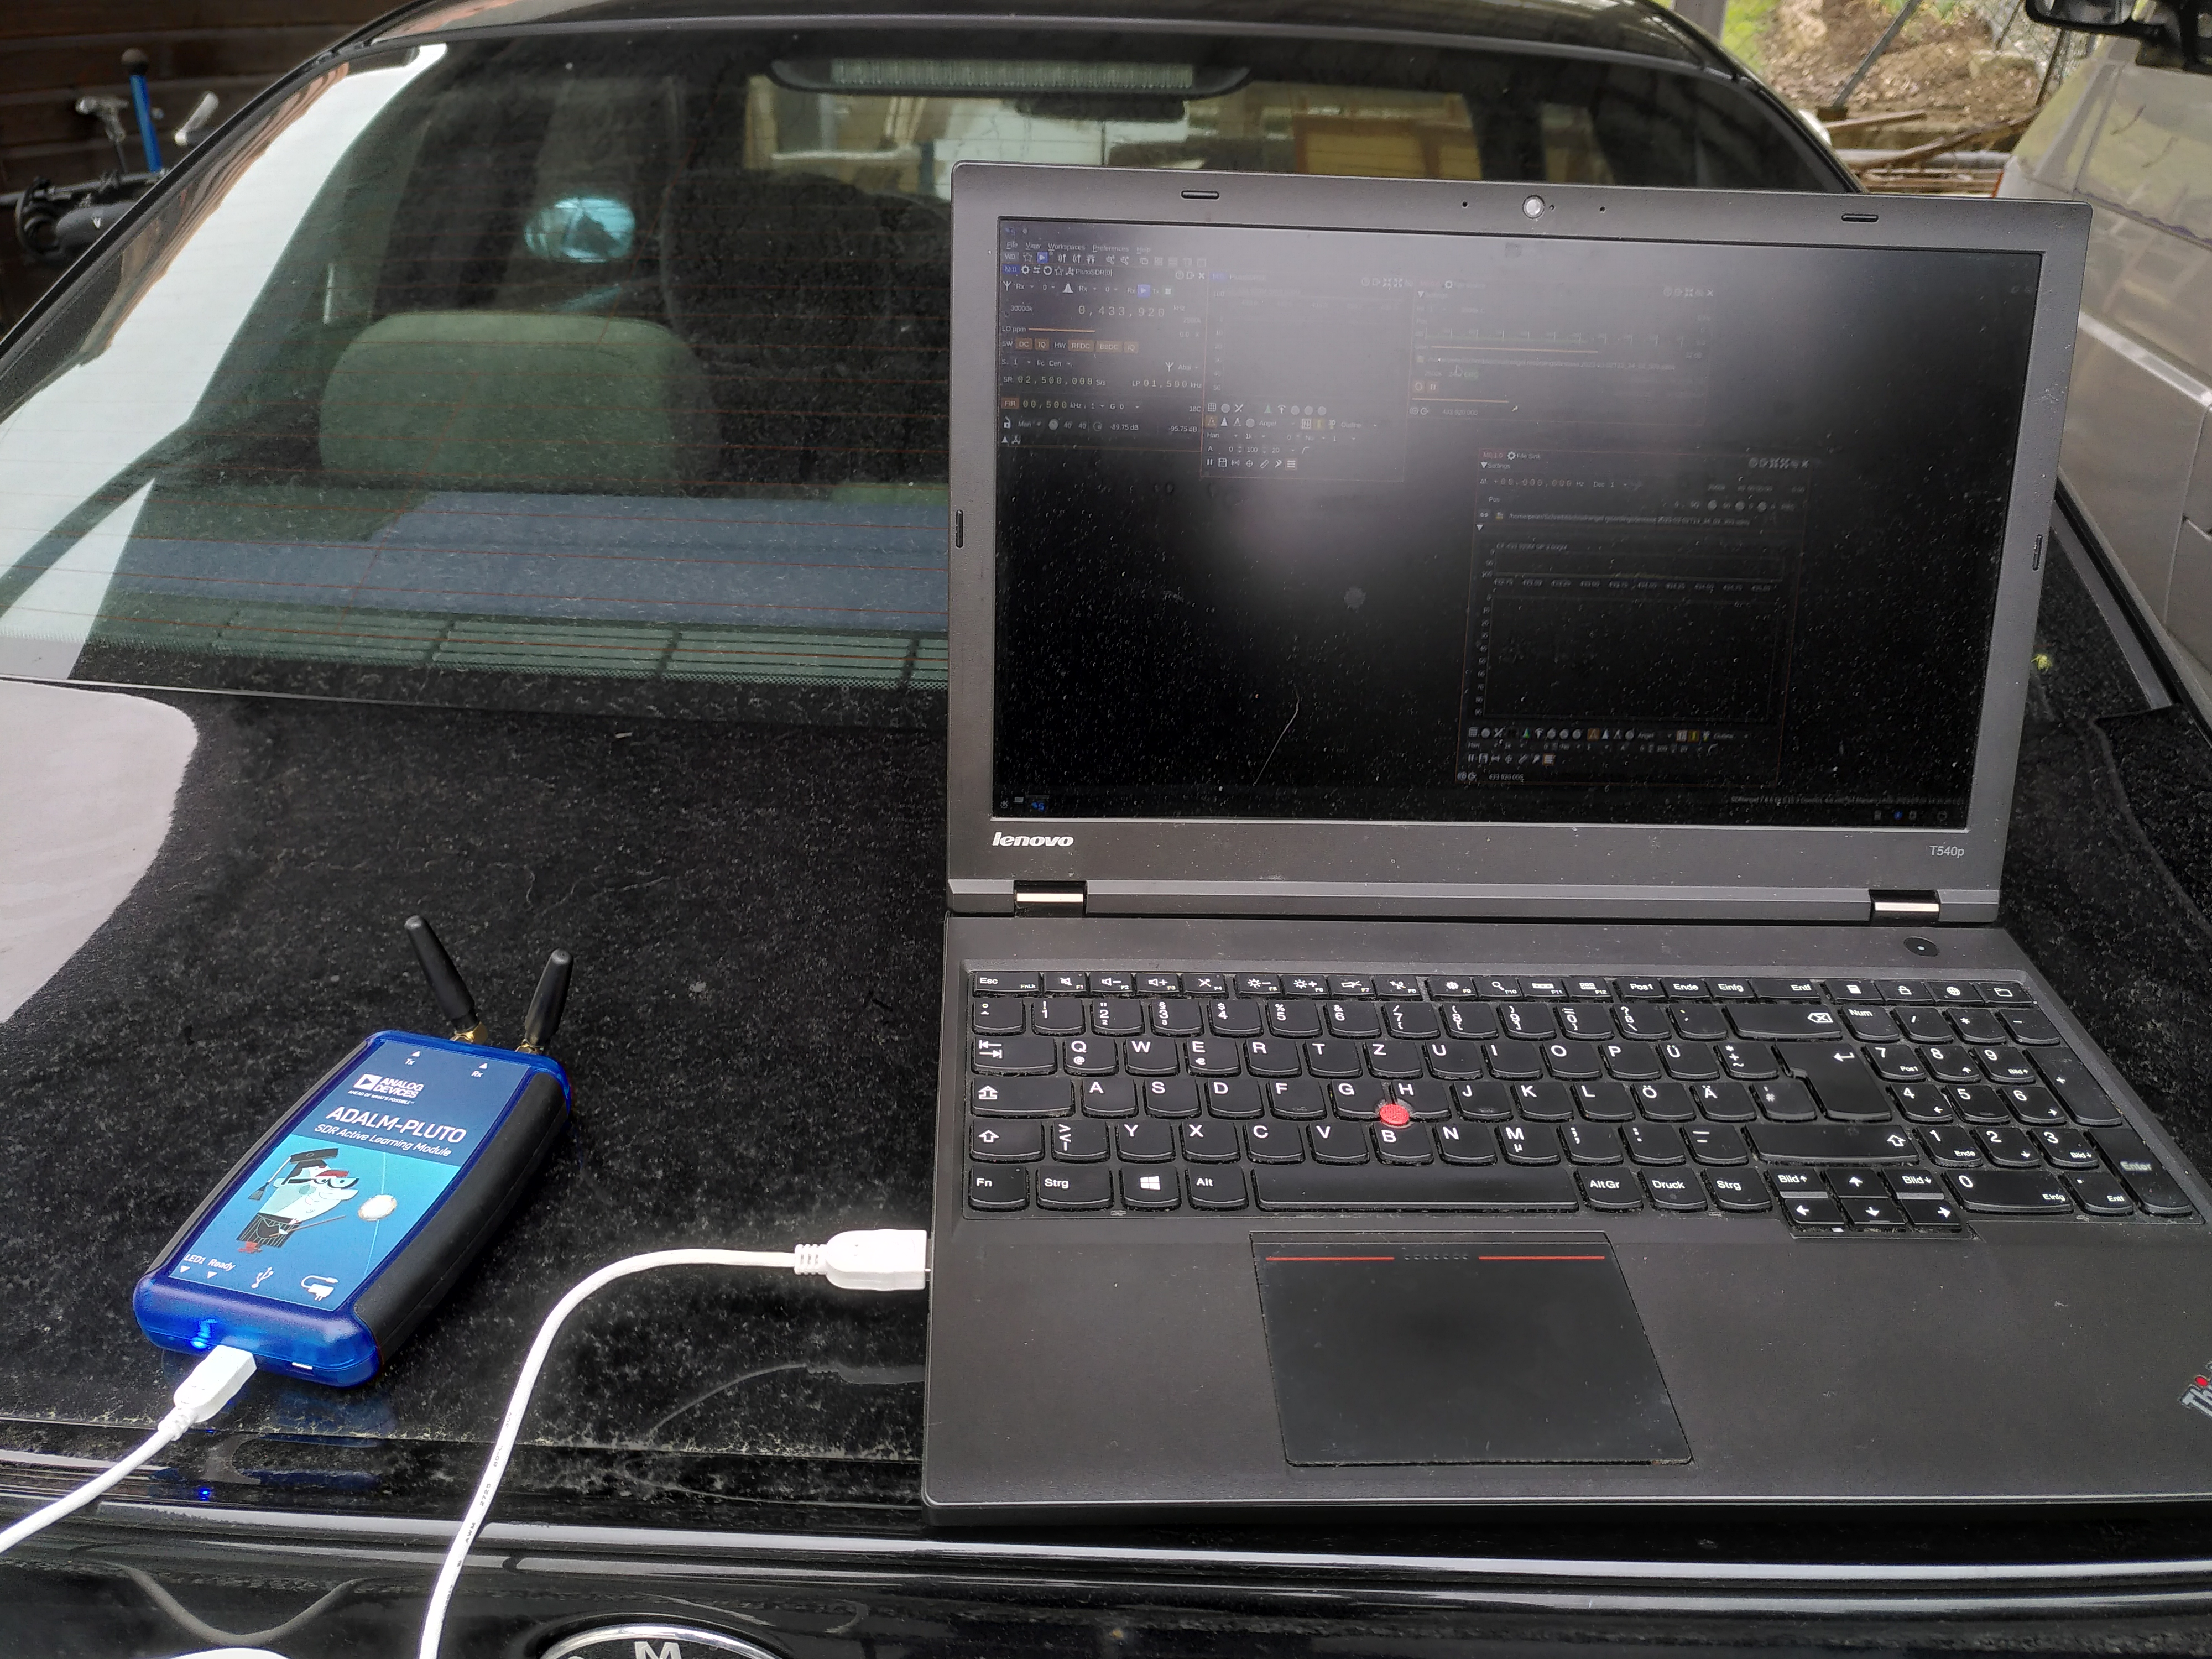
\includegraphics[width=.8\linewidth]{img/demonstration3/signal_transmission_setup.jpg}
        \caption{Host computer and SDR on the vehicle's trunk}
    \end{center}
\end{figure}

The captured signal can then be transmitted to the car via the ``File Channel Source'' Plugin. First, the File Dialog has to be opened via the ``Open I/Q record file'' button. This opens the OS specific file dialog, where a previously recorded .sdriq or .wav file can be selected. Once this file is loaded, the signal can be transmitted by enabling transmissions on the device and clicking the ``Play/Pause'' button. 
The gain of the transmitted signal can be adjusted with the ``Gain'' slider just below. This way the signal strength can be boosted until the transmission almost reaches the 0dB mark. Depending on the noise level and the distance between the key and the SDR during capture, this may be necessary in order for the signal to reach the vehicle.

\begin{figure}[!h]
    \begin{center}
        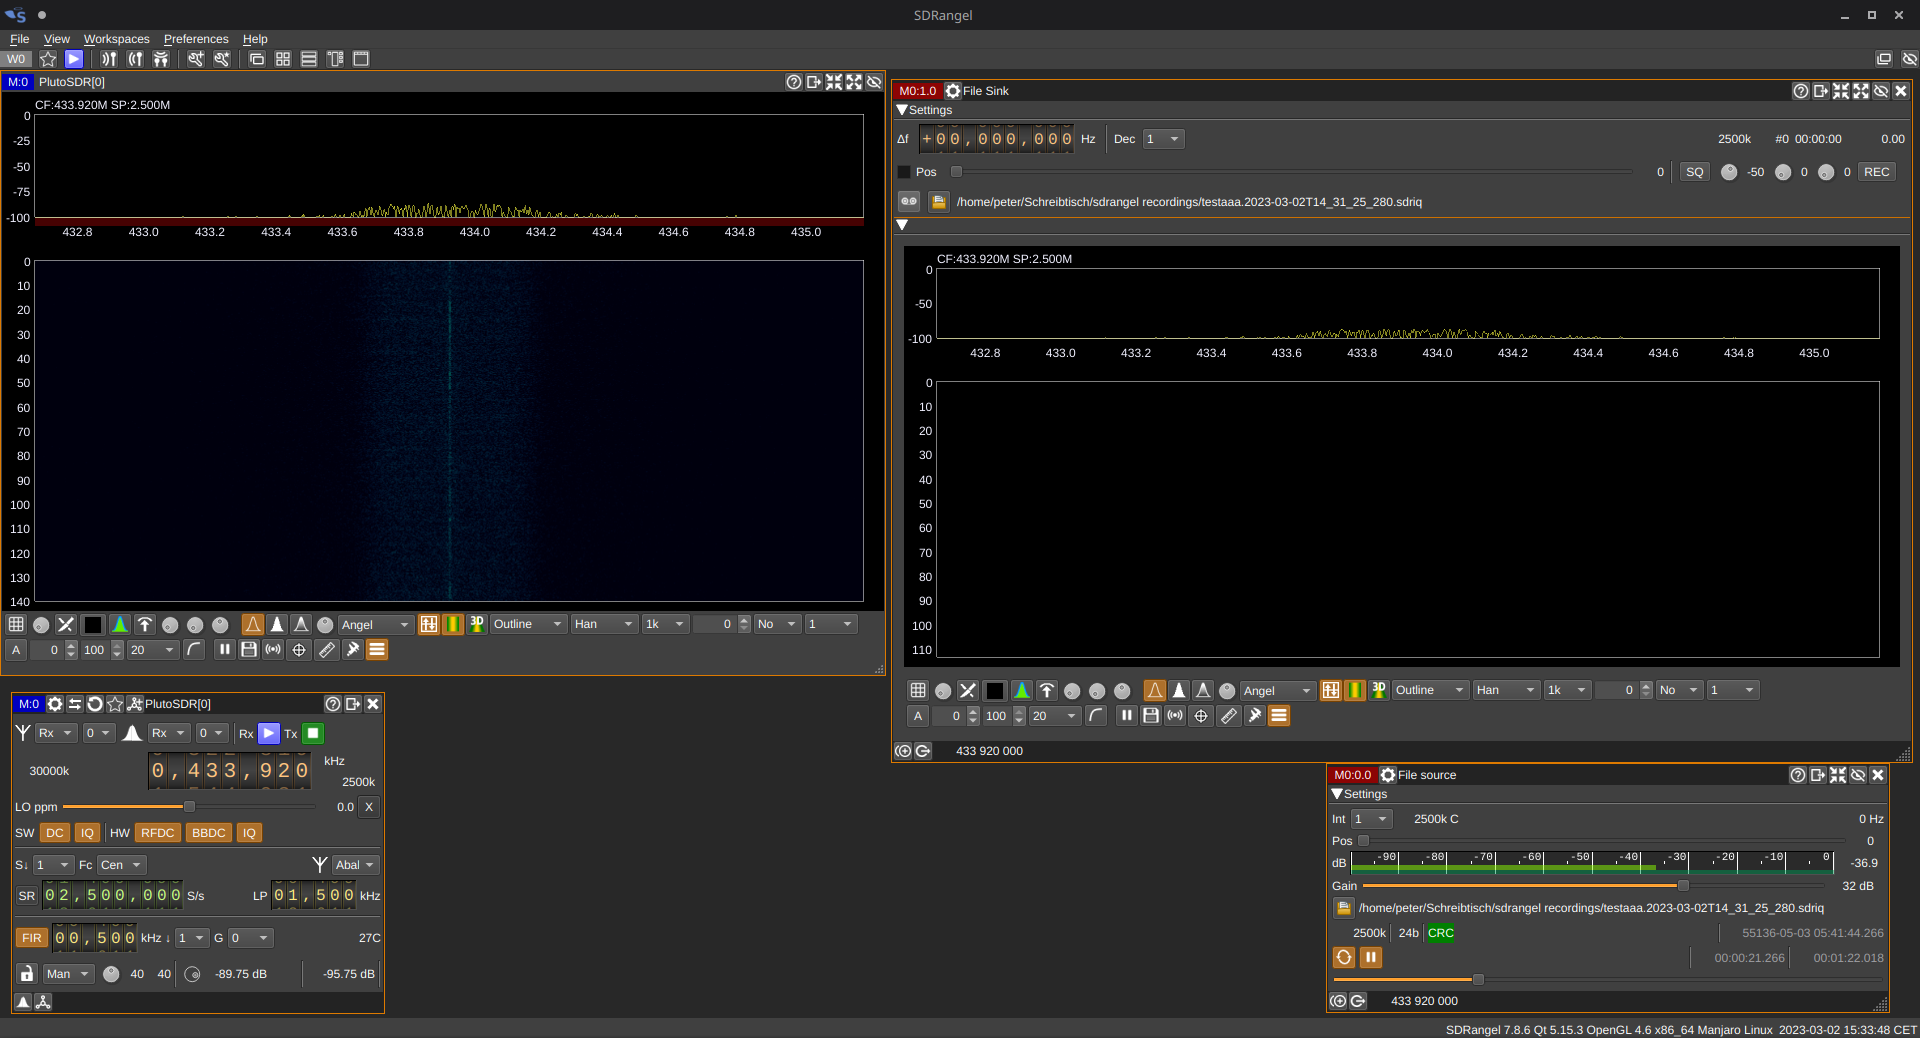
\includegraphics[width=.8\linewidth]{img/demonstration3/playback_signal.png}
        \caption{SDRangel while playing back the signal}
    \end{center}
\end{figure}

After adjusting the gain to 32dB, the signal was received and the vehicle unlocked.

\begin{figure}[!h]
    \begin{center}
        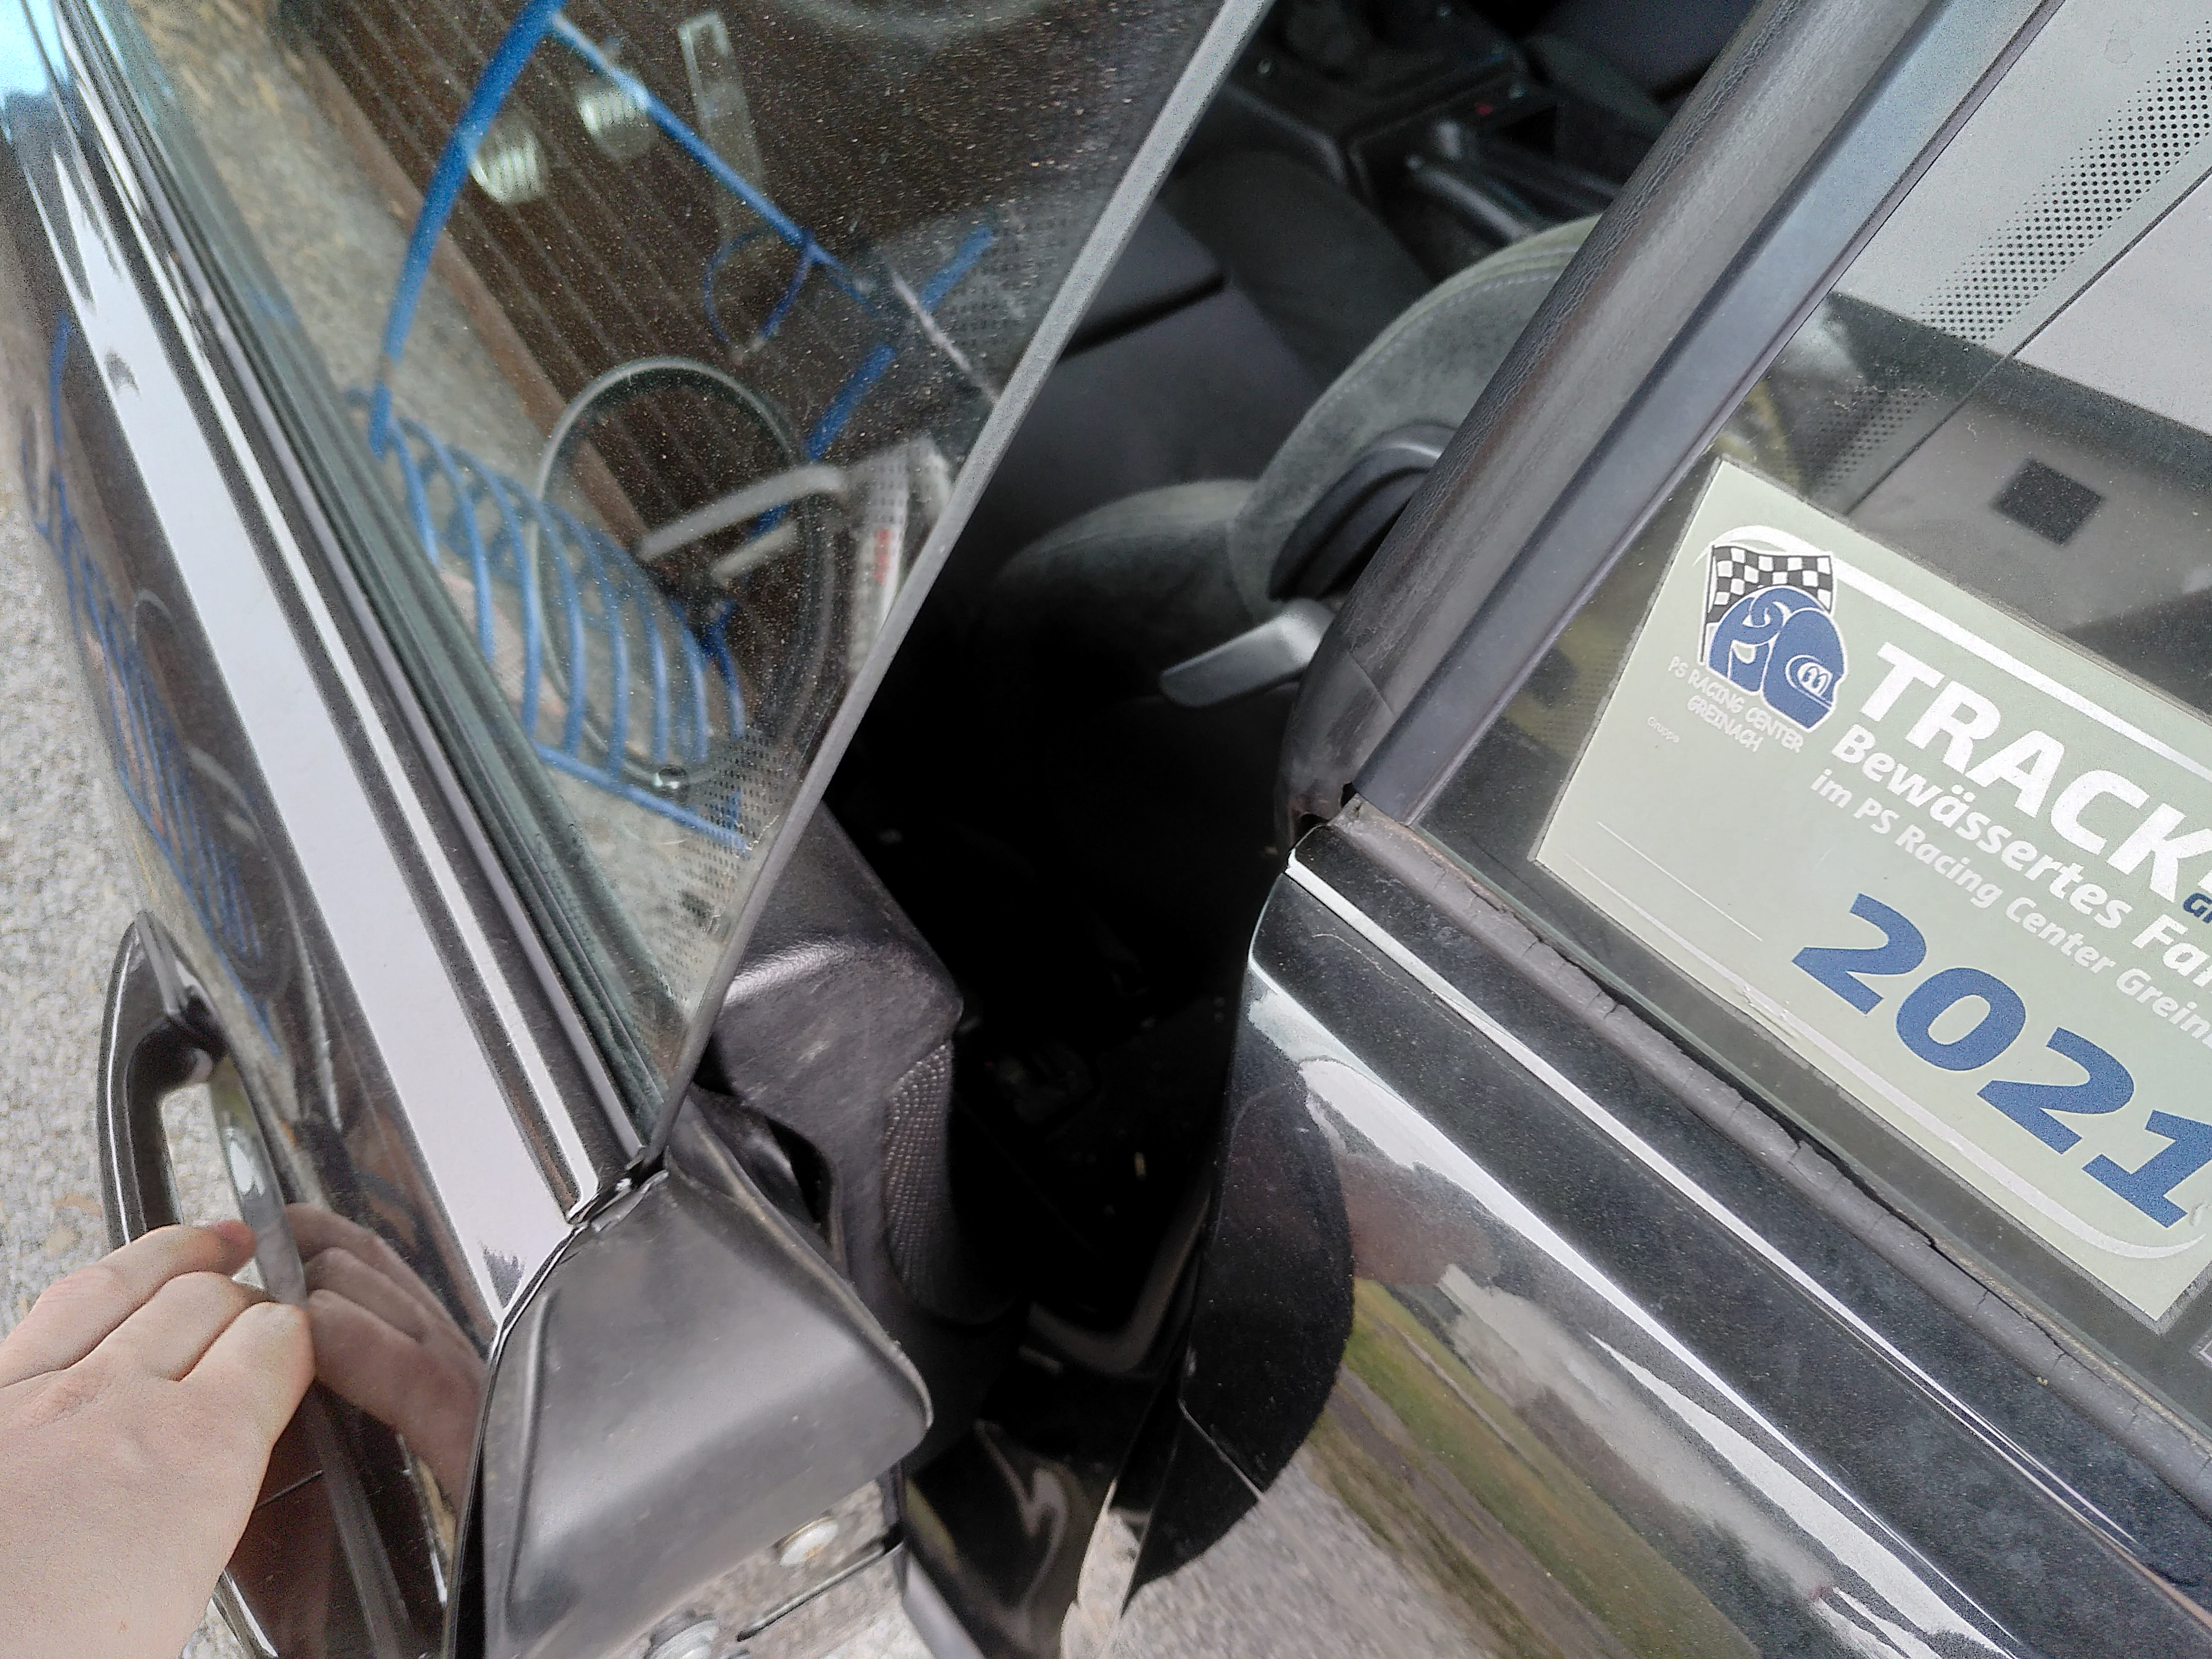
\includegraphics[width=.8\linewidth]{img/demonstration3/unlocked_door.jpg}
        \caption{The vehicle with the unlocked door}
    \end{center}
\end{figure}

\subsection{Rolljam}
Of course the scenario in which an attack has posession of the key,captures a signal without the victim knowing and is subsequently able to use the signal before the attacker returns to his vehicle is somewhat unlikely.
A much more practical approach would be to capture an unlock signal without needing the key entirely. To do this, an attack might simply wait until the victim approaches their vehicle to unlock it and then simultaniously block the key's signal from reaching the car and record it to the host PC. To the owner of the vehicle, it might appear as if the unlock signal has simply failed to reach. Once the victim tries for a second time, the signal is again blocked, but the previously recorded signal is sent from the attackers PC to the car instead, while the key's second unlock signal is recorded again.
This causes the car to be one step behind the key as far as rolling codes are concerned. The attacker now has a working unlock signal in their posession to use at any time.
Such an attack is also called Rolljam. In order to execute it the SDR or some other kind of jamming device needs to transmit at the exact frequency that the key transmits at, with enough power and the same type of modulation in order to overpower the keys signal and prevent it from reaching its destination. Usually, a white noise signal is used for this purpose. %TODO fact check

\subsection{Defeating Rolling Code}
As previously mentioned, all vehicles using the Rolling Code Cryptography generate a new code based on every new key press deterministically out of the last used code. Usually car manufacturers contract semiconductor companies to design and implement these cryptographic systems, or buy integrated Circuits already designed for this purpose. 

One such contractor is NXP, which has offered their HiTag2 Transponder IC since 1996, which has been adopted in more than 200 different car models by at least 34 manufacturers. It is mainly used as an additional immobilizer unit that prevents the car from not starting when the key is not present.

Unfortunately it relies on a proprietary stream cipher, which contains several weakpoints. Researchers were able to devise multiple attacks on this IC and the cipher in particular and are now able retrieve the 48 Bit key of any immobilizer unit with this chip within 360 seconds or less.
\cite{verdult2012gone}

Often, the Hitag2 key is shared between the immobilizer unit and the key remote. This is the case in ICs like PCF7946/7947. This fact was exploited by a different research group in order to completely reverse-engineer the rolling code scheme of these remotes and published in a paper in 2016.

With knowledge of the Hitag2 cipher and a novel attack method described in this paper, an attacker is potentially able to recover the key just by eavesdropping between 4-8 keypresses. Using this this key and knowledge of the Rolling Code system, the authors of the paper were able to unlock a number of cars from different manufacturers made between 2004 and 2016.\cite{garcia2016lock}

Keeloq is another cryptographic scheme which was broken by researchers. It is a block cipher, which is often used for security relevant applications like remote keyless entry systems or immobilizers.
Using cryptographic analysis as well as sidechannel attacks like Power analysis a skilled attacker is able to recover the key. All they need is physical access to the key and equipment to measure its power draw during button presses. Once they are in posession of the cipher key, they are able to decode a message and retrieve the rolling code counter value as well as the unique ID. With this, they can essentially clone the remote and unlock the vehicle as many times as they want. %TODO cite power analysis

Vehicle makers like Volkswagen also sometimes implement their own cipher. The same research group mentioned above was able to identify at least 7 different Rolling Code ciphers used by the company just by eavesdropping key communications. By further studying the PCBs found in Volkswagen remotes and analyzing the firmware on a number of ECUs of VW cars, the group was able to determine that a large number of vehicles by the brand made in the last 20 years was secured with only a small number of cryptographic keys. This means that an attacker with knowledge of these keys might be able to decode the unique ID of the remote and the rolling counter value from a single eavesdropped key signal. With this information, an attacker can then send signals to lock an unlock the vehicle as many times as desired.\cite{garcia2016lock}

\subsection{Relay Attacks}
With modern passive keyless entry systems, archaeic button pushing is no longer required at all. The key now simply needs to be anywhere near the vehicle to start exchanging messages with it. Combined with the fact that these systems usually send multiple messages back and forth between the key and the car in order to authenticate, the effort required to conduct a replay attack is much greater than in simple remote-based keyless entry systems. 

Instead ``Relay-Attacks'' can be used in order to trick the vehicle and the key into thinking they are much closer to each other than they are in reality. This is achieved by planting a transponder device near the key, which picks up messages it sends and sending it to another transponder device, which is placed near the car. The key and the vehicle then communicate as if they were next to one another, while the transponders intermittently carry the signal over a large distance for example via Internet. The only limitation of this attack is strict time limits depending on the implementation of the PKES system.
%TODO cite relay paper oder so und neu schreiben weil das suckt




% -----~* BIBLIOGRAPHY *~-----
\newpage
%add to table of contents
\addtocounter{page}{1}
%\addcontentsline{toc}{chapter}{Bibliography}
\addtocounter{page}{-1}

\printbibliography[heading=bibintoc]

\end{document}

%TODO Title case in headlines und labels
